\Opensolutionfile{solution_file}[solutions/sols_020]
% в квадратных скобках фактическое имя файла

\chapter{Парный МНК без матриц}


\begin{problem}
Рассмотрим модель $y_t=\b_1+\b_2 \cdot t + \e_t$, где ошибки $\e_t$ независимы и равномерны на $[-1;1]$. С помощью симуляций на компьютере оцените и постройте график функции плотности для $\hb_1$, $\hb_2$, $\hs^2$, $\hVar(\hb_1)$, $\hVar(\hb_2)$ и $\hCov(\hb_1,\hb_2)$.


\begin{sol}
Даешь симуляции!

\begin{minted}[mathescape,
               linenos,
               numbersep=5pt,
               frame=lines,
               framesep=2mm]{r}
n <- 100 # количество наблюдений
m <- 100 # можно менять количество прогонов
         # и радоваться!
x <- rnorm(n, 5, 1)

b1 <- rep(0, m)
b2 <- rep(0, m)
sHatSquared <- rep(0, m)
varB1 <- rep(0, m)
varB2 <- rep(0, m)
Cov <- rep(0, m)

for(i in 1:m) {
  y <- 1 + 2 * x + runif(n, -1, 1)       # остатки распределены как надо
  b1[i] <- coef(lm(y ~ x))[[1]]
  b2[i] <- coef(lm(y ~ x))[[2]]
  sHatSquared[i] <- sum((summary(lm(y ~ x))$resid)^2) / (n - 2)
  varB1[i] <- vcov(lm(y ~ x))[1, 1]
  varB2[i] <- vcov(lm(y ~ x))[2, 2]
  Cov[i] <- vcov(lm(y ~ x))[1, 2]
}

palette(c("ForestGreen", "olivedrab", "SkyBlue", "tomato3", "navy", "brown"))
par(mfrow = c(2, 3))

toPlot <- data.frame(b1 = b1, b2 = b2, sHatSquared = sHatSquared,
                     varB1 = varB1, varB2 = varB2, Cov = Cov)

for(i in 1:ncol(toPlot))           # построим все одним махом
{
  hist(toPlot[, i], prob = TRUE, main = "",
       xlab = colnames(toPlot)[i], ylim = c(0, max(density(toPlot[, i])$y)) )
  lines(density(toPlot[, i]), col = i, lwd = 4)
}
\end{minted}

\begin{minipage}{0.6\textwidth}
\begin{center}
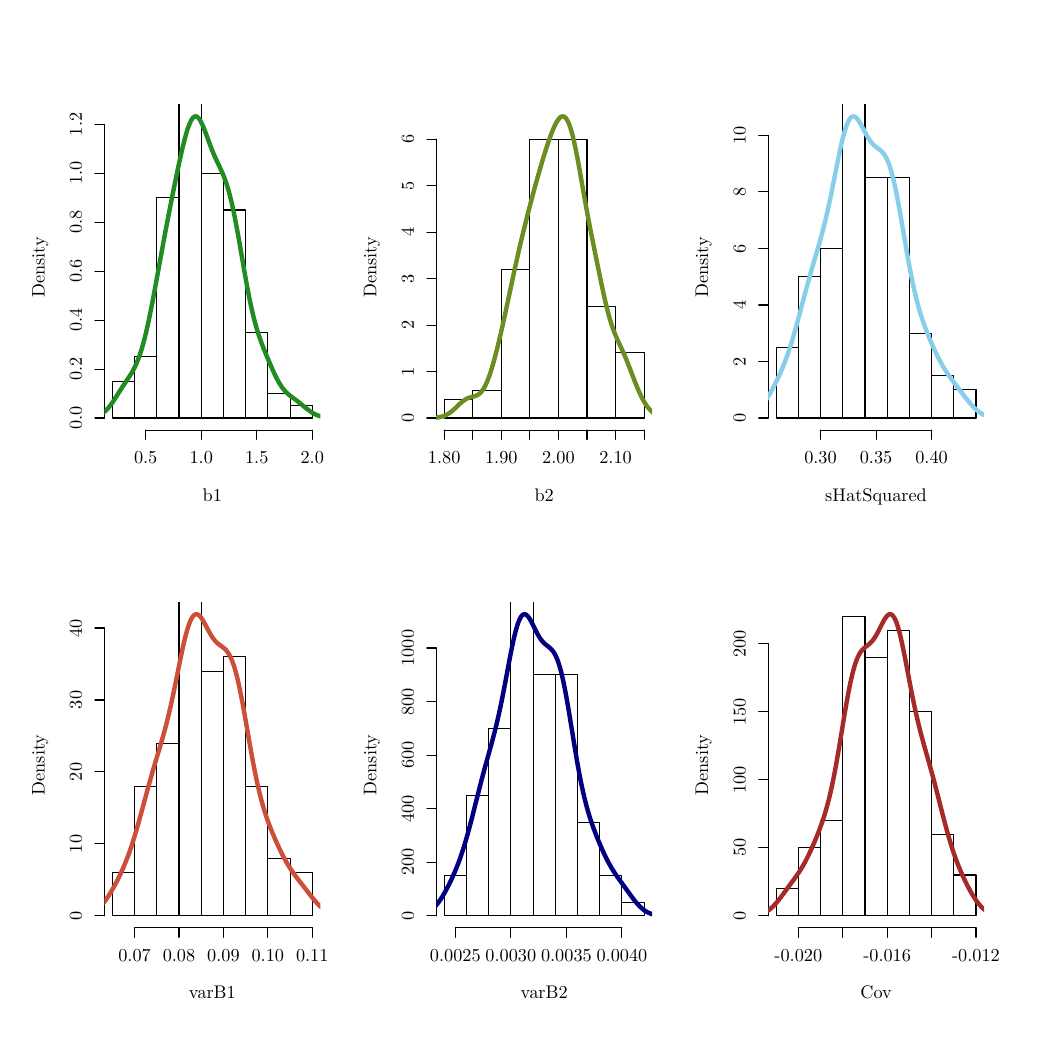
\begin{tikzpicture}[scale = 0.025]
% Created by tikzDevice version 0.12 on 2019-05-26 19:57:10
% !TEX encoding = UTF-8 Unicode
\definecolor{fillColor}{RGB}{255,255,255}
\path[use as bounding box,fill=fillColor,fill opacity=0.00] (0,0) rectangle (505.89,505.89);
\begin{scope}
\path[clip] (  0.00,252.94) rectangle (168.63,505.89);
\definecolor{drawColor}{RGB}{0,0,0}

\node[text=drawColor,anchor=base,inner sep=0pt, outer sep=0pt, scale=  0.66] at ( 93.82,265.30) {b1};

\node[text=drawColor,rotate= 90.00,anchor=base,inner sep=0pt, outer sep=0pt, scale=  0.66] at (  8.55,384.17) {Density};
\end{scope}
\begin{scope}
\path[clip] (  0.00,  0.00) rectangle (505.89,505.89);
\definecolor{drawColor}{RGB}{0,0,0}

\path[draw=drawColor,line width= 0.4pt,line join=round,line cap=round] ( 59.96,301.42) -- (144.61,301.42);

\path[draw=drawColor,line width= 0.4pt,line join=round,line cap=round] ( 59.96,301.42) -- ( 59.96,296.66);

\path[draw=drawColor,line width= 0.4pt,line join=round,line cap=round] ( 88.18,301.42) -- ( 88.18,296.66);

\path[draw=drawColor,line width= 0.4pt,line join=round,line cap=round] (116.39,301.42) -- (116.39,296.66);

\path[draw=drawColor,line width= 0.4pt,line join=round,line cap=round] (144.61,301.42) -- (144.61,296.66);

\node[text=drawColor,anchor=base,inner sep=0pt, outer sep=0pt, scale=  0.66] at ( 59.96,284.31) {0.5};

\node[text=drawColor,anchor=base,inner sep=0pt, outer sep=0pt, scale=  0.66] at ( 88.18,284.31) {1.0};

\node[text=drawColor,anchor=base,inner sep=0pt, outer sep=0pt, scale=  0.66] at (116.39,284.31) {1.5};

\node[text=drawColor,anchor=base,inner sep=0pt, outer sep=0pt, scale=  0.66] at (144.61,284.31) {2.0};

\path[draw=drawColor,line width= 0.4pt,line join=round,line cap=round] ( 38.97,307.55) -- ( 38.97,456.77);

\path[draw=drawColor,line width= 0.4pt,line join=round,line cap=round] ( 38.97,307.55) -- ( 34.21,307.55);

\path[draw=drawColor,line width= 0.4pt,line join=round,line cap=round] ( 38.97,332.42) -- ( 34.21,332.42);

\path[draw=drawColor,line width= 0.4pt,line join=round,line cap=round] ( 38.97,357.29) -- ( 34.21,357.29);

\path[draw=drawColor,line width= 0.4pt,line join=round,line cap=round] ( 38.97,382.16) -- ( 34.21,382.16);

\path[draw=drawColor,line width= 0.4pt,line join=round,line cap=round] ( 38.97,407.03) -- ( 34.21,407.03);

\path[draw=drawColor,line width= 0.4pt,line join=round,line cap=round] ( 38.97,431.90) -- ( 34.21,431.90);

\path[draw=drawColor,line width= 0.4pt,line join=round,line cap=round] ( 38.97,456.77) -- ( 34.21,456.77);

\node[text=drawColor,rotate= 90.00,anchor=base,inner sep=0pt, outer sep=0pt, scale=  0.66] at ( 27.56,307.55) {0.0};

\node[text=drawColor,rotate= 90.00,anchor=base,inner sep=0pt, outer sep=0pt, scale=  0.66] at ( 27.56,332.42) {0.2};

\node[text=drawColor,rotate= 90.00,anchor=base,inner sep=0pt, outer sep=0pt, scale=  0.66] at ( 27.56,357.29) {0.4};

\node[text=drawColor,rotate= 90.00,anchor=base,inner sep=0pt, outer sep=0pt, scale=  0.66] at ( 27.56,382.16) {0.6};

\node[text=drawColor,rotate= 90.00,anchor=base,inner sep=0pt, outer sep=0pt, scale=  0.66] at ( 27.56,407.03) {0.8};

\node[text=drawColor,rotate= 90.00,anchor=base,inner sep=0pt, outer sep=0pt, scale=  0.66] at ( 27.56,431.90) {1.0};

\node[text=drawColor,rotate= 90.00,anchor=base,inner sep=0pt, outer sep=0pt, scale=  0.66] at ( 27.56,456.77) {1.2};
\end{scope}
\begin{scope}
\path[clip] ( 38.97,301.42) rectangle (148.67,466.92);
\definecolor{drawColor}{RGB}{0,0,0}

\path[draw=drawColor,line width= 0.4pt,line join=round,line cap=round] ( 43.03,307.55) rectangle ( 54.32,326.20);

\path[draw=drawColor,line width= 0.4pt,line join=round,line cap=round] ( 54.32,307.55) rectangle ( 65.60,338.63);

\path[draw=drawColor,line width= 0.4pt,line join=round,line cap=round] ( 65.60,307.55) rectangle ( 76.89,419.46);

\path[draw=drawColor,line width= 0.4pt,line join=round,line cap=round] ( 76.89,307.55) rectangle ( 88.18,475.42);

\path[draw=drawColor,line width= 0.4pt,line join=round,line cap=round] ( 88.18,307.55) rectangle ( 99.46,431.90);

\path[draw=drawColor,line width= 0.4pt,line join=round,line cap=round] ( 99.46,307.55) rectangle (110.75,413.24);

\path[draw=drawColor,line width= 0.4pt,line join=round,line cap=round] (110.75,307.55) rectangle (122.04,351.07);

\path[draw=drawColor,line width= 0.4pt,line join=round,line cap=round] (122.04,307.55) rectangle (133.32,319.98);

\path[draw=drawColor,line width= 0.4pt,line join=round,line cap=round] (133.32,307.55) rectangle (144.61,313.76);
\definecolor{drawColor}{RGB}{34,139,34}

\path[draw=drawColor,line width= 1.6pt,line join=round,line cap=round] ( 30.21,307.66) --
	( 30.46,307.67) --
	( 30.71,307.69) --
	( 30.95,307.71) --
	( 31.20,307.73) --
	( 31.44,307.75) --
	( 31.69,307.77) --
	( 31.93,307.80) --
	( 32.18,307.83) --
	( 32.42,307.86) --
	( 32.67,307.89) --
	( 32.91,307.93) --
	( 33.16,307.97) --
	( 33.41,308.02) --
	( 33.65,308.07) --
	( 33.90,308.12) --
	( 34.14,308.18) --
	( 34.39,308.24) --
	( 34.63,308.31) --
	( 34.88,308.38) --
	( 35.12,308.46) --
	( 35.37,308.54) --
	( 35.62,308.63) --
	( 35.86,308.73) --
	( 36.11,308.84) --
	( 36.35,308.95) --
	( 36.60,309.07) --
	( 36.84,309.19) --
	( 37.09,309.33) --
	( 37.33,309.47) --
	( 37.58,309.62) --
	( 37.82,309.79) --
	( 38.07,309.95) --
	( 38.32,310.13) --
	( 38.56,310.32) --
	( 38.81,310.52) --
	( 39.05,310.72) --
	( 39.30,310.94) --
	( 39.54,311.17) --
	( 39.79,311.41) --
	( 40.03,311.65) --
	( 40.28,311.91) --
	( 40.53,312.17) --
	( 40.77,312.45) --
	( 41.02,312.73) --
	( 41.26,313.03) --
	( 41.51,313.33) --
	( 41.75,313.64) --
	( 42.00,313.96) --
	( 42.24,314.29) --
	( 42.49,314.62) --
	( 42.73,314.96) --
	( 42.98,315.31) --
	( 43.23,315.67) --
	( 43.47,316.03) --
	( 43.72,316.40) --
	( 43.96,316.77) --
	( 44.21,317.15) --
	( 44.45,317.53) --
	( 44.70,317.91) --
	( 44.94,318.29) --
	( 45.19,318.68) --
	( 45.44,319.07) --
	( 45.68,319.46) --
	( 45.93,319.85) --
	( 46.17,320.24) --
	( 46.42,320.63) --
	( 46.66,321.02) --
	( 46.91,321.40) --
	( 47.15,321.79) --
	( 47.40,322.17) --
	( 47.65,322.56) --
	( 47.89,322.94) --
	( 48.14,323.31) --
	( 48.38,323.69) --
	( 48.63,324.06) --
	( 48.87,324.43) --
	( 49.12,324.80) --
	( 49.36,325.17) --
	( 49.61,325.53) --
	( 49.85,325.90) --
	( 50.10,326.26) --
	( 50.35,326.63) --
	( 50.59,326.99) --
	( 50.84,327.36) --
	( 51.08,327.72) --
	( 51.33,328.10) --
	( 51.57,328.47) --
	( 51.82,328.85) --
	( 52.06,329.23) --
	( 52.31,329.63) --
	( 52.56,330.02) --
	( 52.80,330.43) --
	( 53.05,330.85) --
	( 53.29,331.28) --
	( 53.54,331.72) --
	( 53.78,332.17) --
	( 54.03,332.64) --
	( 54.27,333.12) --
	( 54.52,333.61) --
	( 54.76,334.13) --
	( 55.01,334.66) --
	( 55.26,335.21) --
	( 55.50,335.78) --
	( 55.75,336.37) --
	( 55.99,336.98) --
	( 56.24,337.62) --
	( 56.48,338.28) --
	( 56.73,338.96) --
	( 56.97,339.66) --
	( 57.22,340.39) --
	( 57.47,341.14) --
	( 57.71,341.92) --
	( 57.96,342.72) --
	( 58.20,343.56) --
	( 58.45,344.41) --
	( 58.69,345.29) --
	( 58.94,346.19) --
	( 59.18,347.12) --
	( 59.43,348.08) --
	( 59.67,349.06) --
	( 59.92,350.06) --
	( 60.17,351.09) --
	( 60.41,352.14) --
	( 60.66,353.21) --
	( 60.90,354.31) --
	( 61.15,355.43) --
	( 61.39,356.56) --
	( 61.64,357.72) --
	( 61.88,358.90) --
	( 62.13,360.09) --
	( 62.38,361.30) --
	( 62.62,362.53) --
	( 62.87,363.78) --
	( 63.11,365.03) --
	( 63.36,366.30) --
	( 63.60,367.59) --
	( 63.85,368.88) --
	( 64.09,370.19) --
	( 64.34,371.50) --
	( 64.58,372.82) --
	( 64.83,374.15) --
	( 65.08,375.48) --
	( 65.32,376.82) --
	( 65.57,378.17) --
	( 65.81,379.51) --
	( 66.06,380.86) --
	( 66.30,382.21) --
	( 66.55,383.57) --
	( 66.79,384.92) --
	( 67.04,386.27) --
	( 67.29,387.62) --
	( 67.53,388.97) --
	( 67.78,390.31) --
	( 68.02,391.65) --
	( 68.27,392.99) --
	( 68.51,394.33) --
	( 68.76,395.66) --
	( 69.00,396.98) --
	( 69.25,398.30) --
	( 69.49,399.62) --
	( 69.74,400.93) --
	( 69.99,402.23) --
	( 70.23,403.53) --
	( 70.48,404.82) --
	( 70.72,406.11) --
	( 70.97,407.39) --
	( 71.21,408.67) --
	( 71.46,409.94) --
	( 71.70,411.21) --
	( 71.95,412.47) --
	( 72.20,413.73) --
	( 72.44,414.98) --
	( 72.69,416.23) --
	( 72.93,417.47) --
	( 73.18,418.71) --
	( 73.42,419.94) --
	( 73.67,421.17) --
	( 73.91,422.39) --
	( 74.16,423.61) --
	( 74.40,424.83) --
	( 74.65,426.04) --
	( 74.90,427.24) --
	( 75.14,428.44) --
	( 75.39,429.63) --
	( 75.63,430.82) --
	( 75.88,432.00) --
	( 76.12,433.18) --
	( 76.37,434.34) --
	( 76.61,435.50) --
	( 76.86,436.65) --
	( 77.11,437.78) --
	( 77.35,438.91) --
	( 77.60,440.03) --
	( 77.84,441.13) --
	( 78.09,442.21) --
	( 78.33,443.29) --
	( 78.58,444.34) --
	( 78.82,445.37) --
	( 79.07,446.39) --
	( 79.32,447.39) --
	( 79.56,448.35) --
	( 79.81,449.30) --
	( 80.05,450.22) --
	( 80.30,451.11) --
	( 80.54,451.97) --
	( 80.79,452.80) --
	( 81.03,453.61) --
	( 81.28,454.36) --
	( 81.52,455.09) --
	( 81.77,455.78) --
	( 82.02,456.43) --
	( 82.26,457.04) --
	( 82.51,457.61) --
	( 82.75,458.13) --
	( 83.00,458.61) --
	( 83.24,459.04) --
	( 83.49,459.43) --
	( 83.73,459.77) --
	( 83.98,460.06) --
	( 84.23,460.30) --
	( 84.47,460.50) --
	( 84.72,460.64) --
	( 84.96,460.74) --
	( 85.21,460.79) --
	( 85.45,460.79) --
	( 85.70,460.74) --
	( 85.94,460.64) --
	( 86.19,460.51) --
	( 86.43,460.31) --
	( 86.68,460.08) --
	( 86.93,459.82) --
	( 87.17,459.50) --
	( 87.42,459.14) --
	( 87.66,458.76) --
	( 87.91,458.33) --
	( 88.15,457.87) --
	( 88.40,457.38) --
	( 88.64,456.86) --
	( 88.89,456.31) --
	( 89.14,455.74) --
	( 89.38,455.16) --
	( 89.63,454.55) --
	( 89.87,453.92) --
	( 90.12,453.28) --
	( 90.36,452.63) --
	( 90.61,451.96) --
	( 90.85,451.30) --
	( 91.10,450.62) --
	( 91.34,449.95) --
	( 91.59,449.27) --
	( 91.84,448.60) --
	( 92.08,447.93) --
	( 92.33,447.26) --
	( 92.57,446.60) --
	( 92.82,445.95) --
	( 93.06,445.30) --
	( 93.31,444.67) --
	( 93.55,444.04) --
	( 93.80,443.43) --
	( 94.05,442.82) --
	( 94.29,442.23) --
	( 94.54,441.65) --
	( 94.78,441.08) --
	( 95.03,440.52) --
	( 95.27,439.96) --
	( 95.52,439.42) --
	( 95.76,438.88) --
	( 96.01,438.36) --
	( 96.25,437.83) --
	( 96.50,437.31) --
	( 96.75,436.80) --
	( 96.99,436.28) --
	( 97.24,435.77) --
	( 97.48,435.25) --
	( 97.73,434.73) --
	( 97.97,434.21) --
	( 98.22,433.67) --
	( 98.46,433.13) --
	( 98.71,432.58) --
	( 98.96,432.02) --
	( 99.20,431.43) --
	( 99.45,430.84) --
	( 99.69,430.23) --
	( 99.94,429.59) --
	(100.18,428.94) --
	(100.43,428.27) --
	(100.67,427.57) --
	(100.92,426.84) --
	(101.16,426.10) --
	(101.41,425.33) --
	(101.66,424.52) --
	(101.90,423.69) --
	(102.15,422.83) --
	(102.39,421.95) --
	(102.64,421.02) --
	(102.88,420.07) --
	(103.13,419.10) --
	(103.37,418.09) --
	(103.62,417.05) --
	(103.87,415.98) --
	(104.11,414.89) --
	(104.36,413.76) --
	(104.60,412.61) --
	(104.85,411.43) --
	(105.09,410.22) --
	(105.34,408.99) --
	(105.58,407.73) --
	(105.83,406.45) --
	(106.07,405.15) --
	(106.32,403.83) --
	(106.57,402.49) --
	(106.81,401.13) --
	(107.06,399.76) --
	(107.30,398.38) --
	(107.55,396.98) --
	(107.79,395.57) --
	(108.04,394.15) --
	(108.28,392.73) --
	(108.53,391.30) --
	(108.78,389.88) --
	(109.02,388.45) --
	(109.27,387.02) --
	(109.51,385.59) --
	(109.76,384.18) --
	(110.00,382.76) --
	(110.25,381.36) --
	(110.49,379.97) --
	(110.74,378.59) --
	(110.99,377.23) --
	(111.23,375.88) --
	(111.48,374.55) --
	(111.72,373.24) --
	(111.97,371.95) --
	(112.21,370.68) --
	(112.46,369.43) --
	(112.70,368.21) --
	(112.95,367.01) --
	(113.19,365.84) --
	(113.44,364.69) --
	(113.69,363.57) --
	(113.93,362.48) --
	(114.18,361.41) --
	(114.42,360.37) --
	(114.67,359.36) --
	(114.91,358.37) --
	(115.16,357.41) --
	(115.40,356.48) --
	(115.65,355.57) --
	(115.90,354.68) --
	(116.14,353.82) --
	(116.39,352.99) --
	(116.63,352.17) --
	(116.88,351.38) --
	(117.12,350.61) --
	(117.37,349.85) --
	(117.61,349.11) --
	(117.86,348.40) --
	(118.10,347.69) --
	(118.35,347.00) --
	(118.60,346.33) --
	(118.84,345.66) --
	(119.09,345.01) --
	(119.33,344.37) --
	(119.58,343.73) --
	(119.82,343.11) --
	(120.07,342.49) --
	(120.31,341.87) --
	(120.56,341.27) --
	(120.81,340.66) --
	(121.05,340.06) --
	(121.30,339.47) --
	(121.54,338.88) --
	(121.79,338.29) --
	(122.03,337.70) --
	(122.28,337.12) --
	(122.52,336.54) --
	(122.77,335.96) --
	(123.01,335.39) --
	(123.26,334.82) --
	(123.51,334.25) --
	(123.75,333.69) --
	(124.00,333.13) --
	(124.24,332.57) --
	(124.49,332.02) --
	(124.73,331.48) --
	(124.98,330.94) --
	(125.22,330.41) --
	(125.47,329.88) --
	(125.72,329.37) --
	(125.96,328.86) --
	(126.21,328.37) --
	(126.45,327.88) --
	(126.70,327.40) --
	(126.94,326.94) --
	(127.19,326.48) --
	(127.43,326.04) --
	(127.68,325.61) --
	(127.92,325.19) --
	(128.17,324.79) --
	(128.42,324.40) --
	(128.66,324.01) --
	(128.91,323.65) --
	(129.15,323.29) --
	(129.40,322.95) --
	(129.64,322.62) --
	(129.89,322.31) --
	(130.13,322.00) --
	(130.38,321.71) --
	(130.63,321.43) --
	(130.87,321.16) --
	(131.12,320.90) --
	(131.36,320.64) --
	(131.61,320.40) --
	(131.85,320.17) --
	(132.10,319.94) --
	(132.34,319.72) --
	(132.59,319.51) --
	(132.83,319.31) --
	(133.08,319.11) --
	(133.33,318.91) --
	(133.57,318.72) --
	(133.82,318.53) --
	(134.06,318.34) --
	(134.31,318.16) --
	(134.55,317.98) --
	(134.80,317.80) --
	(135.04,317.62) --
	(135.29,317.44) --
	(135.54,317.25) --
	(135.78,317.07) --
	(136.03,316.89) --
	(136.27,316.71) --
	(136.52,316.52) --
	(136.76,316.34) --
	(137.01,316.15) --
	(137.25,315.96) --
	(137.50,315.77) --
	(137.74,315.57) --
	(137.99,315.38) --
	(138.24,315.18) --
	(138.48,314.98) --
	(138.73,314.78) --
	(138.97,314.58) --
	(139.22,314.38) --
	(139.46,314.17) --
	(139.71,313.97) --
	(139.95,313.77) --
	(140.20,313.56) --
	(140.45,313.36) --
	(140.69,313.16) --
	(140.94,312.95) --
	(141.18,312.75) --
	(141.43,312.55) --
	(141.67,312.36) --
	(141.92,312.16) --
	(142.16,311.97) --
	(142.41,311.78) --
	(142.66,311.59) --
	(142.90,311.41) --
	(143.15,311.23) --
	(143.39,311.06) --
	(143.64,310.89) --
	(143.88,310.72) --
	(144.13,310.56) --
	(144.37,310.40) --
	(144.62,310.25) --
	(144.86,310.10) --
	(145.11,309.95) --
	(145.36,309.82) --
	(145.60,309.68) --
	(145.85,309.55) --
	(146.09,309.43) --
	(146.34,309.31) --
	(146.58,309.20) --
	(146.83,309.09) --
	(147.07,308.99) --
	(147.32,308.89) --
	(147.57,308.80) --
	(147.81,308.71) --
	(148.06,308.63) --
	(148.30,308.55) --
	(148.55,308.48) --
	(148.79,308.41) --
	(149.04,308.34) --
	(149.28,308.28) --
	(149.53,308.22) --
	(149.77,308.17) --
	(150.02,308.12) --
	(150.27,308.07) --
	(150.51,308.03) --
	(150.76,307.98) --
	(151.00,307.95) --
	(151.25,307.91) --
	(151.49,307.88) --
	(151.74,307.85) --
	(151.98,307.82) --
	(152.23,307.79) --
	(152.48,307.77) --
	(152.72,307.75) --
	(152.97,307.73) --
	(153.21,307.71) --
	(153.46,307.69) --
	(153.70,307.68) --
	(153.95,307.67) --
	(154.19,307.65) --
	(154.44,307.64) --
	(154.68,307.63) --
	(154.93,307.62) --
	(155.18,307.61) --
	(155.42,307.61) --
	(155.67,307.60);
\end{scope}
\begin{scope}
\path[clip] (168.63,252.94) rectangle (337.26,505.89);
\definecolor{drawColor}{RGB}{0,0,0}

\node[text=drawColor,anchor=base,inner sep=0pt, outer sep=0pt, scale=  0.66] at (262.45,265.30) {b2};

\node[text=drawColor,rotate= 90.00,anchor=base,inner sep=0pt, outer sep=0pt, scale=  0.66] at (177.18,384.17) {Density};
\end{scope}
\begin{scope}
\path[clip] (  0.00,  0.00) rectangle (505.89,505.89);
\definecolor{drawColor}{RGB}{0,0,0}

\path[draw=drawColor,line width= 0.4pt,line join=round,line cap=round] (211.66,301.42) -- (313.24,301.42);

\path[draw=drawColor,line width= 0.4pt,line join=round,line cap=round] (211.66,301.42) -- (211.66,296.66);

\path[draw=drawColor,line width= 0.4pt,line join=round,line cap=round] (226.17,301.42) -- (226.17,296.66);

\path[draw=drawColor,line width= 0.4pt,line join=round,line cap=round] (240.68,301.42) -- (240.68,296.66);

\path[draw=drawColor,line width= 0.4pt,line join=round,line cap=round] (255.19,301.42) -- (255.19,296.66);

\path[draw=drawColor,line width= 0.4pt,line join=round,line cap=round] (269.70,301.42) -- (269.70,296.66);

\path[draw=drawColor,line width= 0.4pt,line join=round,line cap=round] (284.22,301.42) -- (284.22,296.66);

\path[draw=drawColor,line width= 0.4pt,line join=round,line cap=round] (298.73,301.42) -- (298.73,296.66);

\path[draw=drawColor,line width= 0.4pt,line join=round,line cap=round] (313.24,301.42) -- (313.24,296.66);

\node[text=drawColor,anchor=base,inner sep=0pt, outer sep=0pt, scale=  0.66] at (211.66,284.31) {1.80};

\node[text=drawColor,anchor=base,inner sep=0pt, outer sep=0pt, scale=  0.66] at (240.68,284.31) {1.90};

\node[text=drawColor,anchor=base,inner sep=0pt, outer sep=0pt, scale=  0.66] at (269.70,284.31) {2.00};

\node[text=drawColor,anchor=base,inner sep=0pt, outer sep=0pt, scale=  0.66] at (298.73,284.31) {2.10};

\path[draw=drawColor,line width= 0.4pt,line join=round,line cap=round] (207.60,307.55) -- (207.60,449.23);

\path[draw=drawColor,line width= 0.4pt,line join=round,line cap=round] (207.60,307.55) -- (202.84,307.55);

\path[draw=drawColor,line width= 0.4pt,line join=round,line cap=round] (207.60,331.16) -- (202.84,331.16);

\path[draw=drawColor,line width= 0.4pt,line join=round,line cap=round] (207.60,354.77) -- (202.84,354.77);

\path[draw=drawColor,line width= 0.4pt,line join=round,line cap=round] (207.60,378.39) -- (202.84,378.39);

\path[draw=drawColor,line width= 0.4pt,line join=round,line cap=round] (207.60,402.00) -- (202.84,402.00);

\path[draw=drawColor,line width= 0.4pt,line join=round,line cap=round] (207.60,425.62) -- (202.84,425.62);

\path[draw=drawColor,line width= 0.4pt,line join=round,line cap=round] (207.60,449.23) -- (202.84,449.23);

\node[text=drawColor,rotate= 90.00,anchor=base,inner sep=0pt, outer sep=0pt, scale=  0.66] at (196.19,307.55) {0};

\node[text=drawColor,rotate= 90.00,anchor=base,inner sep=0pt, outer sep=0pt, scale=  0.66] at (196.19,331.16) {1};

\node[text=drawColor,rotate= 90.00,anchor=base,inner sep=0pt, outer sep=0pt, scale=  0.66] at (196.19,354.77) {2};

\node[text=drawColor,rotate= 90.00,anchor=base,inner sep=0pt, outer sep=0pt, scale=  0.66] at (196.19,378.39) {3};

\node[text=drawColor,rotate= 90.00,anchor=base,inner sep=0pt, outer sep=0pt, scale=  0.66] at (196.19,402.00) {4};

\node[text=drawColor,rotate= 90.00,anchor=base,inner sep=0pt, outer sep=0pt, scale=  0.66] at (196.19,425.62) {5};

\node[text=drawColor,rotate= 90.00,anchor=base,inner sep=0pt, outer sep=0pt, scale=  0.66] at (196.19,449.23) {6};
\end{scope}
\begin{scope}
\path[clip] (207.60,301.42) rectangle (317.30,466.92);
\definecolor{drawColor}{RGB}{0,0,0}

\path[draw=drawColor,line width= 0.4pt,line join=round,line cap=round] (211.66,307.55) rectangle (226.17,316.99);

\path[draw=drawColor,line width= 0.4pt,line join=round,line cap=round] (226.17,307.55) rectangle (240.68,321.71);

\path[draw=drawColor,line width= 0.4pt,line join=round,line cap=round] (240.68,307.55) rectangle (255.19,383.11);

\path[draw=drawColor,line width= 0.4pt,line join=round,line cap=round] (255.19,307.55) rectangle (269.70,449.23);

\path[draw=drawColor,line width= 0.4pt,line join=round,line cap=round] (269.70,307.55) rectangle (284.22,449.23);

\path[draw=drawColor,line width= 0.4pt,line join=round,line cap=round] (284.22,307.55) rectangle (298.73,364.22);

\path[draw=drawColor,line width= 0.4pt,line join=round,line cap=round] (298.73,307.55) rectangle (313.24,340.61);
\definecolor{drawColor}{RGB}{107,142,35}

\path[draw=drawColor,line width= 1.6pt,line join=round,line cap=round] (205.14,307.61) --
	(205.38,307.62) --
	(205.62,307.63) --
	(205.86,307.64) --
	(206.10,307.65) --
	(206.34,307.67) --
	(206.58,307.68) --
	(206.82,307.70) --
	(207.06,307.72) --
	(207.30,307.74) --
	(207.54,307.76) --
	(207.78,307.78) --
	(208.01,307.81) --
	(208.25,307.84) --
	(208.49,307.87) --
	(208.73,307.91) --
	(208.97,307.95) --
	(209.21,307.99) --
	(209.45,308.04) --
	(209.69,308.08) --
	(209.93,308.14) --
	(210.17,308.20) --
	(210.41,308.26) --
	(210.65,308.33) --
	(210.89,308.40) --
	(211.13,308.48) --
	(211.36,308.56) --
	(211.60,308.65) --
	(211.84,308.74) --
	(212.08,308.84) --
	(212.32,308.95) --
	(212.56,309.06) --
	(212.80,309.18) --
	(213.04,309.31) --
	(213.28,309.44) --
	(213.52,309.58) --
	(213.76,309.73) --
	(214.00,309.88) --
	(214.24,310.04) --
	(214.48,310.20) --
	(214.72,310.38) --
	(214.95,310.55) --
	(215.19,310.74) --
	(215.43,310.93) --
	(215.67,311.13) --
	(215.91,311.33) --
	(216.15,311.54) --
	(216.39,311.75) --
	(216.63,311.96) --
	(216.87,312.18) --
	(217.11,312.41) --
	(217.35,312.63) --
	(217.59,312.86) --
	(217.83,313.09) --
	(218.07,313.32) --
	(218.30,313.55) --
	(218.54,313.78) --
	(218.78,314.01) --
	(219.02,314.24) --
	(219.26,314.47) --
	(219.50,314.69) --
	(219.74,314.91) --
	(219.98,315.13) --
	(220.22,315.34) --
	(220.46,315.55) --
	(220.70,315.75) --
	(220.94,315.94) --
	(221.18,316.13) --
	(221.42,316.31) --
	(221.66,316.48) --
	(221.89,316.65) --
	(222.13,316.80) --
	(222.37,316.95) --
	(222.61,317.09) --
	(222.85,317.22) --
	(223.09,317.34) --
	(223.33,317.46) --
	(223.57,317.57) --
	(223.81,317.67) --
	(224.05,317.76) --
	(224.29,317.84) --
	(224.53,317.92) --
	(224.77,318.00) --
	(225.01,318.07) --
	(225.24,318.13) --
	(225.48,318.19) --
	(225.72,318.26) --
	(225.96,318.32) --
	(226.20,318.38) --
	(226.44,318.44) --
	(226.68,318.50) --
	(226.92,318.57) --
	(227.16,318.64) --
	(227.40,318.72) --
	(227.64,318.81) --
	(227.88,318.90) --
	(228.12,319.00) --
	(228.36,319.12) --
	(228.60,319.25) --
	(228.83,319.39) --
	(229.07,319.55) --
	(229.31,319.73) --
	(229.55,319.92) --
	(229.79,320.12) --
	(230.03,320.35) --
	(230.27,320.60) --
	(230.51,320.87) --
	(230.75,321.16) --
	(230.99,321.48) --
	(231.23,321.81) --
	(231.47,322.16) --
	(231.71,322.55) --
	(231.95,322.96) --
	(232.18,323.39) --
	(232.42,323.84) --
	(232.66,324.32) --
	(232.90,324.83) --
	(233.14,325.35) --
	(233.38,325.91) --
	(233.62,326.48) --
	(233.86,327.08) --
	(234.10,327.70) --
	(234.34,328.35) --
	(234.58,329.02) --
	(234.82,329.71) --
	(235.06,330.42) --
	(235.30,331.15) --
	(235.54,331.91) --
	(235.77,332.67) --
	(236.01,333.47) --
	(236.25,334.28) --
	(236.49,335.10) --
	(236.73,335.94) --
	(236.97,336.80) --
	(237.21,337.68) --
	(237.45,338.57) --
	(237.69,339.47) --
	(237.93,340.39) --
	(238.17,341.32) --
	(238.41,342.26) --
	(238.65,343.22) --
	(238.89,344.19) --
	(239.12,345.17) --
	(239.36,346.16) --
	(239.60,347.16) --
	(239.84,348.17) --
	(240.08,349.19) --
	(240.32,350.22) --
	(240.56,351.25) --
	(240.80,352.30) --
	(241.04,353.35) --
	(241.28,354.41) --
	(241.52,355.48) --
	(241.76,356.56) --
	(242.00,357.64) --
	(242.24,358.73) --
	(242.48,359.82) --
	(242.71,360.92) --
	(242.95,362.03) --
	(243.19,363.14) --
	(243.43,364.25) --
	(243.67,365.36) --
	(243.91,366.48) --
	(244.15,367.60) --
	(244.39,368.73) --
	(244.63,369.85) --
	(244.87,370.98) --
	(245.11,372.10) --
	(245.35,373.23) --
	(245.59,374.36) --
	(245.83,375.48) --
	(246.06,376.60) --
	(246.30,377.72) --
	(246.54,378.84) --
	(246.78,379.95) --
	(247.02,381.06) --
	(247.26,382.17) --
	(247.50,383.27) --
	(247.74,384.37) --
	(247.98,385.46) --
	(248.22,386.54) --
	(248.46,387.62) --
	(248.70,388.70) --
	(248.94,389.76) --
	(249.18,390.82) --
	(249.42,391.87) --
	(249.65,392.92) --
	(249.89,393.96) --
	(250.13,394.99) --
	(250.37,396.02) --
	(250.61,397.03) --
	(250.85,398.05) --
	(251.09,399.05) --
	(251.33,400.05) --
	(251.57,401.04) --
	(251.81,402.02) --
	(252.05,403.00) --
	(252.29,403.98) --
	(252.53,404.94) --
	(252.77,405.90) --
	(253.01,406.86) --
	(253.24,407.81) --
	(253.48,408.76) --
	(253.72,409.70) --
	(253.96,410.64) --
	(254.20,411.57) --
	(254.44,412.50) --
	(254.68,413.42) --
	(254.92,414.34) --
	(255.16,415.26) --
	(255.40,416.17) --
	(255.64,417.08) --
	(255.88,417.98) --
	(256.12,418.88) --
	(256.36,419.78) --
	(256.59,420.67) --
	(256.83,421.56) --
	(257.07,422.45) --
	(257.31,423.33) --
	(257.55,424.21) --
	(257.79,425.09) --
	(258.03,425.96) --
	(258.27,426.82) --
	(258.51,427.69) --
	(258.75,428.54) --
	(258.99,429.40) --
	(259.23,430.25) --
	(259.47,431.09) --
	(259.71,431.93) --
	(259.95,432.77) --
	(260.18,433.60) --
	(260.42,434.43) --
	(260.66,435.25) --
	(260.90,436.06) --
	(261.14,436.87) --
	(261.38,437.68) --
	(261.62,438.48) --
	(261.86,439.27) --
	(262.10,440.06) --
	(262.34,440.84) --
	(262.58,441.61) --
	(262.82,442.38) --
	(263.06,443.14) --
	(263.30,443.90) --
	(263.53,444.64) --
	(263.77,445.38) --
	(264.01,446.11) --
	(264.25,446.83) --
	(264.49,447.54) --
	(264.73,448.24) --
	(264.97,448.92) --
	(265.21,449.60) --
	(265.45,450.27) --
	(265.69,450.92) --
	(265.93,451.57) --
	(266.17,452.20) --
	(266.41,452.81) --
	(266.65,453.40) --
	(266.89,453.99) --
	(267.12,454.56) --
	(267.36,455.10) --
	(267.60,455.63) --
	(267.84,456.14) --
	(268.08,456.63) --
	(268.32,457.10) --
	(268.56,457.54) --
	(268.80,457.97) --
	(269.04,458.36) --
	(269.28,458.73) --
	(269.52,459.08) --
	(269.76,459.40) --
	(270.00,459.68) --
	(270.24,459.94) --
	(270.47,460.17) --
	(270.71,460.36) --
	(270.95,460.52) --
	(271.19,460.64) --
	(271.43,460.74) --
	(271.67,460.78) --
	(271.91,460.79) --
	(272.15,460.77) --
	(272.39,460.71) --
	(272.63,460.59) --
	(272.87,460.44) --
	(273.11,460.25) --
	(273.35,460.01) --
	(273.59,459.72) --
	(273.83,459.39) --
	(274.06,459.02) --
	(274.30,458.60) --
	(274.54,458.12) --
	(274.78,457.61) --
	(275.02,457.05) --
	(275.26,456.44) --
	(275.50,455.78) --
	(275.74,455.08) --
	(275.98,454.33) --
	(276.22,453.53) --
	(276.46,452.69) --
	(276.70,451.81) --
	(276.94,450.88) --
	(277.18,449.91) --
	(277.41,448.91) --
	(277.65,447.87) --
	(277.89,446.78) --
	(278.13,445.67) --
	(278.37,444.52) --
	(278.61,443.35) --
	(278.85,442.14) --
	(279.09,440.91) --
	(279.33,439.66) --
	(279.57,438.38) --
	(279.81,437.08) --
	(280.05,435.77) --
	(280.29,434.44) --
	(280.53,433.10) --
	(280.77,431.76) --
	(281.00,430.40) --
	(281.24,429.04) --
	(281.48,427.68) --
	(281.72,426.31) --
	(281.96,424.95) --
	(282.20,423.59) --
	(282.44,422.23) --
	(282.68,420.87) --
	(282.92,419.53) --
	(283.16,418.19) --
	(283.40,416.86) --
	(283.64,415.54) --
	(283.88,414.23) --
	(284.12,412.93) --
	(284.35,411.63) --
	(284.59,410.35) --
	(284.83,409.08) --
	(285.07,407.82) --
	(285.31,406.57) --
	(285.55,405.33) --
	(285.79,404.10) --
	(286.03,402.88) --
	(286.27,401.66) --
	(286.51,400.45) --
	(286.75,399.25) --
	(286.99,398.05) --
	(287.23,396.86) --
	(287.47,395.67) --
	(287.71,394.49) --
	(287.94,393.30) --
	(288.18,392.12) --
	(288.42,390.95) --
	(288.66,389.77) --
	(288.90,388.59) --
	(289.14,387.42) --
	(289.38,386.24) --
	(289.62,385.07) --
	(289.86,383.90) --
	(290.10,382.73) --
	(290.34,381.57) --
	(290.58,380.40) --
	(290.82,379.24) --
	(291.06,378.09) --
	(291.29,376.94) --
	(291.53,375.80) --
	(291.77,374.66) --
	(292.01,373.54) --
	(292.25,372.42) --
	(292.49,371.32) --
	(292.73,370.23) --
	(292.97,369.15) --
	(293.21,368.09) --
	(293.45,367.05) --
	(293.69,366.03) --
	(293.93,365.02) --
	(294.17,364.03) --
	(294.41,363.07) --
	(294.65,362.12) --
	(294.88,361.20) --
	(295.12,360.30) --
	(295.36,359.43) --
	(295.60,358.58) --
	(295.84,357.75) --
	(296.08,356.95) --
	(296.32,356.17) --
	(296.56,355.41) --
	(296.80,354.68) --
	(297.04,353.97) --
	(297.28,353.29) --
	(297.52,352.61) --
	(297.76,351.97) --
	(298.00,351.34) --
	(298.23,350.73) --
	(298.47,350.13) --
	(298.71,349.55) --
	(298.95,348.99) --
	(299.19,348.43) --
	(299.43,347.88) --
	(299.67,347.35) --
	(299.91,346.82) --
	(300.15,346.30) --
	(300.39,345.78) --
	(300.63,345.26) --
	(300.87,344.75) --
	(301.11,344.24) --
	(301.35,343.72) --
	(301.59,343.20) --
	(301.82,342.69) --
	(302.06,342.16) --
	(302.30,341.64) --
	(302.54,341.10) --
	(302.78,340.56) --
	(303.02,340.02) --
	(303.26,339.46) --
	(303.50,338.91) --
	(303.74,338.34) --
	(303.98,337.77) --
	(304.22,337.18) --
	(304.46,336.60) --
	(304.70,336.00) --
	(304.94,335.40) --
	(305.17,334.79) --
	(305.41,334.18) --
	(305.65,333.56) --
	(305.89,332.94) --
	(306.13,332.32) --
	(306.37,331.69) --
	(306.61,331.06) --
	(306.85,330.43) --
	(307.09,329.80) --
	(307.33,329.17) --
	(307.57,328.55) --
	(307.81,327.92) --
	(308.05,327.30) --
	(308.29,326.68) --
	(308.53,326.07) --
	(308.76,325.46) --
	(309.00,324.85) --
	(309.24,324.26) --
	(309.48,323.67) --
	(309.72,323.09) --
	(309.96,322.52) --
	(310.20,321.96) --
	(310.44,321.41) --
	(310.68,320.86) --
	(310.92,320.33) --
	(311.16,319.82) --
	(311.40,319.31) --
	(311.64,318.81) --
	(311.88,318.32) --
	(312.11,317.85) --
	(312.35,317.39) --
	(312.59,316.94) --
	(312.83,316.51) --
	(313.07,316.08) --
	(313.31,315.67) --
	(313.55,315.28) --
	(313.79,314.89) --
	(314.03,314.52) --
	(314.27,314.16) --
	(314.51,313.81) --
	(314.75,313.48) --
	(314.99,313.16) --
	(315.23,312.85) --
	(315.47,312.55) --
	(315.70,312.26) --
	(315.94,311.99) --
	(316.18,311.73) --
	(316.42,311.48) --
	(316.66,311.24) --
	(316.90,311.01) --
	(317.14,310.79) --
	(317.38,310.58) --
	(317.62,310.38) --
	(317.86,310.19) --
	(318.10,310.02) --
	(318.34,309.85) --
	(318.58,309.68) --
	(318.82,309.53) --
	(319.05,309.39) --
	(319.29,309.26) --
	(319.53,309.13) --
	(319.77,309.01) --
	(320.01,308.90) --
	(320.25,308.79) --
	(320.49,308.69) --
	(320.73,308.60) --
	(320.97,308.51) --
	(321.21,308.43) --
	(321.45,308.36) --
	(321.69,308.29) --
	(321.93,308.23) --
	(322.17,308.17) --
	(322.41,308.11) --
	(322.64,308.06) --
	(322.88,308.01) --
	(323.12,307.97) --
	(323.36,307.93) --
	(323.60,307.89) --
	(323.84,307.86) --
	(324.08,307.83) --
	(324.32,307.80) --
	(324.56,307.77) --
	(324.80,307.75) --
	(325.04,307.73) --
	(325.28,307.71) --
	(325.52,307.69) --
	(325.76,307.68) --
	(325.99,307.66) --
	(326.23,307.65) --
	(326.47,307.64) --
	(326.71,307.63) --
	(326.95,307.62) --
	(327.19,307.61) --
	(327.43,307.60);
\end{scope}
\begin{scope}
\path[clip] (337.26,252.94) rectangle (505.89,505.89);
\definecolor{drawColor}{RGB}{0,0,0}

\node[text=drawColor,anchor=base,inner sep=0pt, outer sep=0pt, scale=  0.66] at (431.08,265.30) {sHatSquared};

\node[text=drawColor,rotate= 90.00,anchor=base,inner sep=0pt, outer sep=0pt, scale=  0.66] at (345.81,384.17) {Density};
\end{scope}
\begin{scope}
\path[clip] (  0.00,  0.00) rectangle (505.89,505.89);
\definecolor{drawColor}{RGB}{0,0,0}

\path[draw=drawColor,line width= 0.4pt,line join=round,line cap=round] (402.86,301.42) -- (459.30,301.42);

\path[draw=drawColor,line width= 0.4pt,line join=round,line cap=round] (402.86,301.42) -- (402.86,296.66);

\path[draw=drawColor,line width= 0.4pt,line join=round,line cap=round] (431.08,301.42) -- (431.08,296.66);

\path[draw=drawColor,line width= 0.4pt,line join=round,line cap=round] (459.30,301.42) -- (459.30,296.66);

\node[text=drawColor,anchor=base,inner sep=0pt, outer sep=0pt, scale=  0.66] at (402.86,284.31) {0.30};

\node[text=drawColor,anchor=base,inner sep=0pt, outer sep=0pt, scale=  0.66] at (431.08,284.31) {0.35};

\node[text=drawColor,anchor=base,inner sep=0pt, outer sep=0pt, scale=  0.66] at (459.30,284.31) {0.40};

\path[draw=drawColor,line width= 0.4pt,line join=round,line cap=round] (376.23,307.55) -- (376.23,451.15);

\path[draw=drawColor,line width= 0.4pt,line join=round,line cap=round] (376.23,307.55) -- (371.47,307.55);

\path[draw=drawColor,line width= 0.4pt,line join=round,line cap=round] (376.23,336.27) -- (371.47,336.27);

\path[draw=drawColor,line width= 0.4pt,line join=round,line cap=round] (376.23,364.99) -- (371.47,364.99);

\path[draw=drawColor,line width= 0.4pt,line join=round,line cap=round] (376.23,393.71) -- (371.47,393.71);

\path[draw=drawColor,line width= 0.4pt,line join=round,line cap=round] (376.23,422.43) -- (371.47,422.43);

\path[draw=drawColor,line width= 0.4pt,line join=round,line cap=round] (376.23,451.15) -- (371.47,451.15);

\node[text=drawColor,rotate= 90.00,anchor=base,inner sep=0pt, outer sep=0pt, scale=  0.66] at (364.82,307.55) {0};

\node[text=drawColor,rotate= 90.00,anchor=base,inner sep=0pt, outer sep=0pt, scale=  0.66] at (364.82,336.27) {2};

\node[text=drawColor,rotate= 90.00,anchor=base,inner sep=0pt, outer sep=0pt, scale=  0.66] at (364.82,364.99) {4};

\node[text=drawColor,rotate= 90.00,anchor=base,inner sep=0pt, outer sep=0pt, scale=  0.66] at (364.82,393.71) {6};

\node[text=drawColor,rotate= 90.00,anchor=base,inner sep=0pt, outer sep=0pt, scale=  0.66] at (364.82,422.43) {8};

\node[text=drawColor,rotate= 90.00,anchor=base,inner sep=0pt, outer sep=0pt, scale=  0.66] at (364.82,451.15) {10};
\end{scope}
\begin{scope}
\path[clip] (376.23,301.42) rectangle (485.93,466.92);
\definecolor{drawColor}{RGB}{0,0,0}

\path[draw=drawColor,line width= 0.4pt,line join=round,line cap=round] (380.29,307.55) rectangle (391.58,343.45);

\path[draw=drawColor,line width= 0.4pt,line join=round,line cap=round] (391.58,307.55) rectangle (402.86,379.35);

\path[draw=drawColor,line width= 0.4pt,line join=round,line cap=round] (402.86,307.55) rectangle (414.15,393.71);

\path[draw=drawColor,line width= 0.4pt,line join=round,line cap=round] (414.15,307.55) rectangle (425.44,508.59);

\path[draw=drawColor,line width= 0.4pt,line join=round,line cap=round] (425.44,307.55) rectangle (436.72,429.61);

\path[draw=drawColor,line width= 0.4pt,line join=round,line cap=round] (436.72,307.55) rectangle (448.01,429.61);

\path[draw=drawColor,line width= 0.4pt,line join=round,line cap=round] (448.01,307.55) rectangle (459.30,350.63);

\path[draw=drawColor,line width= 0.4pt,line join=round,line cap=round] (459.30,307.55) rectangle (470.58,329.09);

\path[draw=drawColor,line width= 0.4pt,line join=round,line cap=round] (470.58,307.55) rectangle (481.87,321.91);
\definecolor{drawColor}{RGB}{135,206,235}

\path[draw=drawColor,line width= 1.6pt,line join=round,line cap=round] (359.09,307.63) --
	(359.35,307.64) --
	(359.61,307.65) --
	(359.88,307.66) --
	(360.14,307.68) --
	(360.41,307.69) --
	(360.67,307.71) --
	(360.94,307.73) --
	(361.20,307.75) --
	(361.47,307.77) --
	(361.73,307.80) --
	(361.99,307.82) --
	(362.26,307.85) --
	(362.52,307.89) --
	(362.79,307.92) --
	(363.05,307.96) --
	(363.32,308.00) --
	(363.58,308.04) --
	(363.85,308.09) --
	(364.11,308.15) --
	(364.37,308.20) --
	(364.64,308.26) --
	(364.90,308.33) --
	(365.17,308.40) --
	(365.43,308.48) --
	(365.70,308.56) --
	(365.96,308.64) --
	(366.22,308.74) --
	(366.49,308.84) --
	(366.75,308.94) --
	(367.02,309.05) --
	(367.28,309.17) --
	(367.55,309.30) --
	(367.81,309.43) --
	(368.08,309.58) --
	(368.34,309.73) --
	(368.60,309.88) --
	(368.87,310.05) --
	(369.13,310.23) --
	(369.40,310.41) --
	(369.66,310.61) --
	(369.93,310.81) --
	(370.19,311.02) --
	(370.46,311.24) --
	(370.72,311.47) --
	(370.98,311.71) --
	(371.25,311.96) --
	(371.51,312.23) --
	(371.78,312.50) --
	(372.04,312.77) --
	(372.31,313.07) --
	(372.57,313.37) --
	(372.83,313.67) --
	(373.10,313.99) --
	(373.36,314.32) --
	(373.63,314.66) --
	(373.89,315.01) --
	(374.16,315.37) --
	(374.42,315.73) --
	(374.69,316.11) --
	(374.95,316.49) --
	(375.21,316.89) --
	(375.48,317.29) --
	(375.74,317.69) --
	(376.01,318.11) --
	(376.27,318.54) --
	(376.54,318.97) --
	(376.80,319.41) --
	(377.07,319.86) --
	(377.33,320.31) --
	(377.59,320.77) --
	(377.86,321.24) --
	(378.12,321.72) --
	(378.39,322.20) --
	(378.65,322.69) --
	(378.92,323.19) --
	(379.18,323.69) --
	(379.45,324.20) --
	(379.71,324.71) --
	(379.97,325.23) --
	(380.24,325.76) --
	(380.50,326.30) --
	(380.77,326.84) --
	(381.03,327.39) --
	(381.30,327.95) --
	(381.56,328.52) --
	(381.82,329.09) --
	(382.09,329.68) --
	(382.35,330.27) --
	(382.62,330.87) --
	(382.88,331.47) --
	(383.15,332.10) --
	(383.41,332.72) --
	(383.68,333.36) --
	(383.94,334.01) --
	(384.20,334.67) --
	(384.47,335.34) --
	(384.73,336.03) --
	(385.00,336.73) --
	(385.26,337.43) --
	(385.53,338.15) --
	(385.79,338.89) --
	(386.06,339.63) --
	(386.32,340.39) --
	(386.58,341.16) --
	(386.85,341.95) --
	(387.11,342.75) --
	(387.38,343.56) --
	(387.64,344.38) --
	(387.91,345.22) --
	(388.17,346.07) --
	(388.43,346.93) --
	(388.70,347.81) --
	(388.96,348.70) --
	(389.23,349.60) --
	(389.49,350.51) --
	(389.76,351.43) --
	(390.02,352.36) --
	(390.29,353.30) --
	(390.55,354.25) --
	(390.81,355.21) --
	(391.08,356.17) --
	(391.34,357.15) --
	(391.61,358.13) --
	(391.87,359.11) --
	(392.14,360.10) --
	(392.40,361.09) --
	(392.67,362.09) --
	(392.93,363.08) --
	(393.19,364.08) --
	(393.46,365.08) --
	(393.72,366.08) --
	(393.99,367.08) --
	(394.25,368.08) --
	(394.52,369.07) --
	(394.78,370.06) --
	(395.05,371.05) --
	(395.31,372.04) --
	(395.57,373.01) --
	(395.84,373.99) --
	(396.10,374.96) --
	(396.37,375.92) --
	(396.63,376.88) --
	(396.90,377.83) --
	(397.16,378.77) --
	(397.42,379.71) --
	(397.69,380.64) --
	(397.95,381.57) --
	(398.22,382.49) --
	(398.48,383.41) --
	(398.75,384.32) --
	(399.01,385.23) --
	(399.28,386.13) --
	(399.54,387.03) --
	(399.80,387.93) --
	(400.07,388.83) --
	(400.33,389.73) --
	(400.60,390.63) --
	(400.86,391.53) --
	(401.13,392.43) --
	(401.39,393.34) --
	(401.66,394.25) --
	(401.92,395.16) --
	(402.18,396.09) --
	(402.45,397.02) --
	(402.71,397.96) --
	(402.98,398.91) --
	(403.24,399.87) --
	(403.51,400.85) --
	(403.77,401.84) --
	(404.03,402.84) --
	(404.30,403.86) --
	(404.56,404.90) --
	(404.83,405.95) --
	(405.09,407.02) --
	(405.36,408.10) --
	(405.62,409.21) --
	(405.89,410.33) --
	(406.15,411.48) --
	(406.41,412.64) --
	(406.68,413.82) --
	(406.94,415.02) --
	(407.21,416.24) --
	(407.47,417.47) --
	(407.74,418.72) --
	(408.00,419.99) --
	(408.27,421.27) --
	(408.53,422.57) --
	(408.79,423.88) --
	(409.06,425.20) --
	(409.32,426.52) --
	(409.59,427.86) --
	(409.85,429.20) --
	(410.12,430.54) --
	(410.38,431.89) --
	(410.65,433.23) --
	(410.91,434.57) --
	(411.17,435.90) --
	(411.44,437.23) --
	(411.70,438.54) --
	(411.97,439.83) --
	(412.23,441.12) --
	(412.50,442.38) --
	(412.76,443.61) --
	(413.02,444.82) --
	(413.29,446.01) --
	(413.55,447.16) --
	(413.82,448.28) --
	(414.08,449.37) --
	(414.35,450.41) --
	(414.61,451.41) --
	(414.88,452.38) --
	(415.14,453.29) --
	(415.40,454.16) --
	(415.67,454.98) --
	(415.93,455.76) --
	(416.20,456.46) --
	(416.46,457.12) --
	(416.73,457.74) --
	(416.99,458.29) --
	(417.26,458.79) --
	(417.52,459.23) --
	(417.78,459.62) --
	(418.05,459.95) --
	(418.31,460.22) --
	(418.58,460.45) --
	(418.84,460.61) --
	(419.11,460.72) --
	(419.37,460.79) --
	(419.63,460.79) --
	(419.90,460.75) --
	(420.16,460.66) --
	(420.43,460.54) --
	(420.69,460.35) --
	(420.96,460.14) --
	(421.22,459.89) --
	(421.49,459.59) --
	(421.75,459.26) --
	(422.01,458.91) --
	(422.28,458.52) --
	(422.54,458.11) --
	(422.81,457.68) --
	(423.07,457.23) --
	(423.34,456.76) --
	(423.60,456.28) --
	(423.87,455.79) --
	(424.13,455.28) --
	(424.39,454.78) --
	(424.66,454.27) --
	(424.92,453.76) --
	(425.19,453.25) --
	(425.45,452.75) --
	(425.72,452.25) --
	(425.98,451.76) --
	(426.25,451.29) --
	(426.51,450.82) --
	(426.77,450.36) --
	(427.04,449.93) --
	(427.30,449.50) --
	(427.57,449.10) --
	(427.83,448.71) --
	(428.10,448.34) --
	(428.36,447.98) --
	(428.62,447.65) --
	(428.89,447.33) --
	(429.15,447.03) --
	(429.42,446.74) --
	(429.68,446.47) --
	(429.95,446.22) --
	(430.21,445.98) --
	(430.48,445.75) --
	(430.74,445.53) --
	(431.00,445.32) --
	(431.27,445.12) --
	(431.53,444.92) --
	(431.80,444.73) --
	(432.06,444.54) --
	(432.33,444.34) --
	(432.59,444.15) --
	(432.86,443.94) --
	(433.12,443.73) --
	(433.38,443.51) --
	(433.65,443.27) --
	(433.91,443.02) --
	(434.18,442.75) --
	(434.44,442.46) --
	(434.71,442.15) --
	(434.97,441.81) --
	(435.24,441.44) --
	(435.50,441.05) --
	(435.76,440.62) --
	(436.03,440.15) --
	(436.29,439.65) --
	(436.56,439.12) --
	(436.82,438.54) --
	(437.09,437.93) --
	(437.35,437.28) --
	(437.61,436.58) --
	(437.88,435.83) --
	(438.14,435.06) --
	(438.41,434.23) --
	(438.67,433.35) --
	(438.94,432.44) --
	(439.20,431.48) --
	(439.47,430.47) --
	(439.73,429.42) --
	(439.99,428.34) --
	(440.26,427.21) --
	(440.52,426.03) --
	(440.79,424.83) --
	(441.05,423.58) --
	(441.32,422.29) --
	(441.58,420.98) --
	(441.85,419.63) --
	(442.11,418.25) --
	(442.37,416.84) --
	(442.64,415.41) --
	(442.90,413.96) --
	(443.17,412.48) --
	(443.43,410.98) --
	(443.70,409.47) --
	(443.96,407.95) --
	(444.22,406.41) --
	(444.49,404.87) --
	(444.75,403.32) --
	(445.02,401.77) --
	(445.28,400.22) --
	(445.55,398.67) --
	(445.81,397.13) --
	(446.08,395.59) --
	(446.34,394.06) --
	(446.60,392.54) --
	(446.87,391.04) --
	(447.13,389.54) --
	(447.40,388.07) --
	(447.66,386.62) --
	(447.93,385.19) --
	(448.19,383.77) --
	(448.46,382.39) --
	(448.72,381.03) --
	(448.98,379.68) --
	(449.25,378.38) --
	(449.51,377.09) --
	(449.78,375.83) --
	(450.04,374.60) --
	(450.31,373.41) --
	(450.57,372.23) --
	(450.84,371.08) --
	(451.10,369.97) --
	(451.36,368.88) --
	(451.63,367.82) --
	(451.89,366.79) --
	(452.16,365.78) --
	(452.42,364.80) --
	(452.69,363.84) --
	(452.95,362.91) --
	(453.21,362.00) --
	(453.48,361.11) --
	(453.74,360.25) --
	(454.01,359.41) --
	(454.27,358.59) --
	(454.54,357.78) --
	(454.80,357.00) --
	(455.07,356.23) --
	(455.33,355.47) --
	(455.59,354.74) --
	(455.86,354.01) --
	(456.12,353.30) --
	(456.39,352.60) --
	(456.65,351.91) --
	(456.92,351.23) --
	(457.18,350.57) --
	(457.45,349.91) --
	(457.71,349.26) --
	(457.97,348.61) --
	(458.24,347.98) --
	(458.50,347.35) --
	(458.77,346.73) --
	(459.03,346.12) --
	(459.30,345.51) --
	(459.56,344.91) --
	(459.82,344.31) --
	(460.09,343.72) --
	(460.35,343.14) --
	(460.62,342.56) --
	(460.88,341.99) --
	(461.15,341.42) --
	(461.41,340.86) --
	(461.68,340.31) --
	(461.94,339.76) --
	(462.20,339.22) --
	(462.47,338.69) --
	(462.73,338.16) --
	(463.00,337.64) --
	(463.26,337.13) --
	(463.53,336.63) --
	(463.79,336.13) --
	(464.06,335.64) --
	(464.32,335.16) --
	(464.58,334.69) --
	(464.85,334.22) --
	(465.11,333.77) --
	(465.38,333.32) --
	(465.64,332.88) --
	(465.91,332.44) --
	(466.17,332.01) --
	(466.44,331.60) --
	(466.70,331.18) --
	(466.96,330.78) --
	(467.23,330.38) --
	(467.49,329.98) --
	(467.76,329.60) --
	(468.02,329.22) --
	(468.29,328.84) --
	(468.55,328.47) --
	(468.81,328.10) --
	(469.08,327.74) --
	(469.34,327.38) --
	(469.61,327.02) --
	(469.87,326.67) --
	(470.14,326.32) --
	(470.40,325.97) --
	(470.67,325.62) --
	(470.93,325.27) --
	(471.19,324.93) --
	(471.46,324.58) --
	(471.72,324.24) --
	(471.99,323.89) --
	(472.25,323.55) --
	(472.52,323.20) --
	(472.78,322.86) --
	(473.05,322.51) --
	(473.31,322.16) --
	(473.57,321.82) --
	(473.84,321.47) --
	(474.10,321.12) --
	(474.37,320.77) --
	(474.63,320.43) --
	(474.90,320.08) --
	(475.16,319.73) --
	(475.42,319.38) --
	(475.69,319.03) --
	(475.95,318.69) --
	(476.22,318.34) --
	(476.48,318.00) --
	(476.75,317.65) --
	(477.01,317.31) --
	(477.28,316.98) --
	(477.54,316.64) --
	(477.80,316.31) --
	(478.07,315.98) --
	(478.33,315.66) --
	(478.60,315.34) --
	(478.86,315.02) --
	(479.13,314.71) --
	(479.39,314.41) --
	(479.66,314.11) --
	(479.92,313.82) --
	(480.18,313.53) --
	(480.45,313.25) --
	(480.71,312.98) --
	(480.98,312.72) --
	(481.24,312.46) --
	(481.51,312.21) --
	(481.77,311.96) --
	(482.04,311.73) --
	(482.30,311.50) --
	(482.56,311.28) --
	(482.83,311.07) --
	(483.09,310.86) --
	(483.36,310.67) --
	(483.62,310.48) --
	(483.89,310.30) --
	(484.15,310.13) --
	(484.41,309.96) --
	(484.68,309.81) --
	(484.94,309.66) --
	(485.21,309.52) --
	(485.47,309.38) --
	(485.74,309.25) --
	(486.00,309.13) --
	(486.27,309.02) --
	(486.53,308.91) --
	(486.79,308.81) --
	(487.06,308.71) --
	(487.32,308.62) --
	(487.59,308.54) --
	(487.85,308.46) --
	(488.12,308.39) --
	(488.38,308.32) --
	(488.65,308.25) --
	(488.91,308.20) --
	(489.17,308.14) --
	(489.44,308.09) --
	(489.70,308.04) --
	(489.97,308.00) --
	(490.23,307.96) --
	(490.50,307.92) --
	(490.76,307.88) --
	(491.02,307.85) --
	(491.29,307.82) --
	(491.55,307.80) --
	(491.82,307.77) --
	(492.08,307.75) --
	(492.35,307.73) --
	(492.61,307.71) --
	(492.88,307.69) --
	(493.14,307.68) --
	(493.40,307.66) --
	(493.67,307.65) --
	(493.93,307.64) --
	(494.20,307.63);
\end{scope}
\begin{scope}
\path[clip] (  0.00,  0.00) rectangle (168.63,252.94);
\definecolor{drawColor}{RGB}{0,0,0}

\node[text=drawColor,anchor=base,inner sep=0pt, outer sep=0pt, scale=  0.66] at ( 93.82, 12.36) {varB1};

\node[text=drawColor,rotate= 90.00,anchor=base,inner sep=0pt, outer sep=0pt, scale=  0.66] at (  8.55,131.22) {Density};
\end{scope}
\begin{scope}
\path[clip] (  0.00,  0.00) rectangle (505.89,505.89);
\definecolor{drawColor}{RGB}{0,0,0}

\path[draw=drawColor,line width= 0.4pt,line join=round,line cap=round] ( 54.32, 48.47) -- (144.61, 48.47);

\path[draw=drawColor,line width= 0.4pt,line join=round,line cap=round] ( 54.32, 48.47) -- ( 54.32, 43.72);

\path[draw=drawColor,line width= 0.4pt,line join=round,line cap=round] ( 76.89, 48.47) -- ( 76.89, 43.72);

\path[draw=drawColor,line width= 0.4pt,line join=round,line cap=round] ( 99.46, 48.47) -- ( 99.46, 43.72);

\path[draw=drawColor,line width= 0.4pt,line join=round,line cap=round] (122.04, 48.47) -- (122.04, 43.72);

\path[draw=drawColor,line width= 0.4pt,line join=round,line cap=round] (144.61, 48.47) -- (144.61, 43.72);

\node[text=drawColor,anchor=base,inner sep=0pt, outer sep=0pt, scale=  0.66] at ( 54.32, 31.36) {0.07};

\node[text=drawColor,anchor=base,inner sep=0pt, outer sep=0pt, scale=  0.66] at ( 76.89, 31.36) {0.08};

\node[text=drawColor,anchor=base,inner sep=0pt, outer sep=0pt, scale=  0.66] at ( 99.46, 31.36) {0.09};

\node[text=drawColor,anchor=base,inner sep=0pt, outer sep=0pt, scale=  0.66] at (122.04, 31.36) {0.10};

\node[text=drawColor,anchor=base,inner sep=0pt, outer sep=0pt, scale=  0.66] at (144.61, 31.36) {0.11};

\path[draw=drawColor,line width= 0.4pt,line join=round,line cap=round] ( 38.97, 54.60) -- ( 38.97,200.83);

\path[draw=drawColor,line width= 0.4pt,line join=round,line cap=round] ( 38.97, 54.60) -- ( 34.21, 54.60);

\path[draw=drawColor,line width= 0.4pt,line join=round,line cap=round] ( 38.97, 91.16) -- ( 34.21, 91.16);

\path[draw=drawColor,line width= 0.4pt,line join=round,line cap=round] ( 38.97,127.72) -- ( 34.21,127.72);

\path[draw=drawColor,line width= 0.4pt,line join=round,line cap=round] ( 38.97,164.27) -- ( 34.21,164.27);

\path[draw=drawColor,line width= 0.4pt,line join=round,line cap=round] ( 38.97,200.83) -- ( 34.21,200.83);

\node[text=drawColor,rotate= 90.00,anchor=base,inner sep=0pt, outer sep=0pt, scale=  0.66] at ( 27.56, 54.60) {0};

\node[text=drawColor,rotate= 90.00,anchor=base,inner sep=0pt, outer sep=0pt, scale=  0.66] at ( 27.56, 91.16) {10};

\node[text=drawColor,rotate= 90.00,anchor=base,inner sep=0pt, outer sep=0pt, scale=  0.66] at ( 27.56,127.72) {20};

\node[text=drawColor,rotate= 90.00,anchor=base,inner sep=0pt, outer sep=0pt, scale=  0.66] at ( 27.56,164.27) {30};

\node[text=drawColor,rotate= 90.00,anchor=base,inner sep=0pt, outer sep=0pt, scale=  0.66] at ( 27.56,200.83) {40};
\end{scope}
\begin{scope}
\path[clip] ( 38.97, 48.47) rectangle (148.67,213.98);
\definecolor{drawColor}{RGB}{0,0,0}

\path[draw=drawColor,line width= 0.4pt,line join=round,line cap=round] ( 43.03, 54.60) rectangle ( 54.32, 76.54);

\path[draw=drawColor,line width= 0.4pt,line join=round,line cap=round] ( 54.32, 54.60) rectangle ( 65.60,120.40);

\path[draw=drawColor,line width= 0.4pt,line join=round,line cap=round] ( 65.60, 54.60) rectangle ( 76.89,142.34);

\path[draw=drawColor,line width= 0.4pt,line join=round,line cap=round] ( 76.89, 54.60) rectangle ( 88.18,237.39);

\path[draw=drawColor,line width= 0.4pt,line join=round,line cap=round] ( 88.18, 54.60) rectangle ( 99.46,178.90);

\path[draw=drawColor,line width= 0.4pt,line join=round,line cap=round] ( 99.46, 54.60) rectangle (110.75,186.21);

\path[draw=drawColor,line width= 0.4pt,line join=round,line cap=round] (110.75, 54.60) rectangle (122.04,120.40);

\path[draw=drawColor,line width= 0.4pt,line join=round,line cap=round] (122.04, 54.60) rectangle (133.32, 83.85);

\path[draw=drawColor,line width= 0.4pt,line join=round,line cap=round] (133.32, 54.60) rectangle (144.61, 76.54);
\definecolor{drawColor}{RGB}{205,79,57}

\path[draw=drawColor,line width= 1.6pt,line join=round,line cap=round] ( 24.13, 54.68) --
	( 24.40, 54.70) --
	( 24.66, 54.71) --
	( 24.93, 54.72) --
	( 25.20, 54.73) --
	( 25.47, 54.75) --
	( 25.74, 54.77) --
	( 26.01, 54.78) --
	( 26.28, 54.80) --
	( 26.55, 54.83) --
	( 26.82, 54.85) --
	( 27.09, 54.88) --
	( 27.36, 54.91) --
	( 27.63, 54.94) --
	( 27.90, 54.98) --
	( 28.16, 55.01) --
	( 28.43, 55.05) --
	( 28.70, 55.10) --
	( 28.97, 55.15) --
	( 29.24, 55.20) --
	( 29.51, 55.26) --
	( 29.78, 55.32) --
	( 30.05, 55.38) --
	( 30.32, 55.45) --
	( 30.59, 55.53) --
	( 30.86, 55.61) --
	( 31.13, 55.70) --
	( 31.40, 55.79) --
	( 31.66, 55.89) --
	( 31.93, 56.00) --
	( 32.20, 56.11) --
	( 32.47, 56.23) --
	( 32.74, 56.35) --
	( 33.01, 56.49) --
	( 33.28, 56.63) --
	( 33.55, 56.78) --
	( 33.82, 56.94) --
	( 34.09, 57.11) --
	( 34.36, 57.28) --
	( 34.63, 57.47) --
	( 34.90, 57.66) --
	( 35.17, 57.86) --
	( 35.43, 58.07) --
	( 35.70, 58.30) --
	( 35.97, 58.53) --
	( 36.24, 58.77) --
	( 36.51, 59.02) --
	( 36.78, 59.28) --
	( 37.05, 59.55) --
	( 37.32, 59.83) --
	( 37.59, 60.12) --
	( 37.86, 60.42) --
	( 38.13, 60.73) --
	( 38.40, 61.05) --
	( 38.67, 61.38) --
	( 38.93, 61.72) --
	( 39.20, 62.06) --
	( 39.47, 62.42) --
	( 39.74, 62.79) --
	( 40.01, 63.16) --
	( 40.28, 63.55) --
	( 40.55, 63.94) --
	( 40.82, 64.34) --
	( 41.09, 64.75) --
	( 41.36, 65.17) --
	( 41.63, 65.59) --
	( 41.90, 66.02) --
	( 42.17, 66.47) --
	( 42.43, 66.91) --
	( 42.70, 67.37) --
	( 42.97, 67.83) --
	( 43.24, 68.30) --
	( 43.51, 68.77) --
	( 43.78, 69.25) --
	( 44.05, 69.74) --
	( 44.32, 70.24) --
	( 44.59, 70.74) --
	( 44.86, 71.25) --
	( 45.13, 71.77) --
	( 45.40, 72.29) --
	( 45.67, 72.82) --
	( 45.94, 73.36) --
	( 46.20, 73.90) --
	( 46.47, 74.45) --
	( 46.74, 75.01) --
	( 47.01, 75.57) --
	( 47.28, 76.15) --
	( 47.55, 76.73) --
	( 47.82, 77.32) --
	( 48.09, 77.92) --
	( 48.36, 78.53) --
	( 48.63, 79.15) --
	( 48.90, 79.78) --
	( 49.17, 80.42) --
	( 49.44, 81.07) --
	( 49.70, 81.73) --
	( 49.97, 82.40) --
	( 50.24, 83.08) --
	( 50.51, 83.78) --
	( 50.78, 84.49) --
	( 51.05, 85.21) --
	( 51.32, 85.94) --
	( 51.59, 86.69) --
	( 51.86, 87.44) --
	( 52.13, 88.22) --
	( 52.40, 89.00) --
	( 52.67, 89.80) --
	( 52.94, 90.61) --
	( 53.21, 91.44) --
	( 53.47, 92.28) --
	( 53.74, 93.12) --
	( 54.01, 93.99) --
	( 54.28, 94.87) --
	( 54.55, 95.75) --
	( 54.82, 96.65) --
	( 55.09, 97.56) --
	( 55.36, 98.48) --
	( 55.63, 99.41) --
	( 55.90,100.36) --
	( 56.17,101.31) --
	( 56.44,102.26) --
	( 56.71,103.23) --
	( 56.97,104.20) --
	( 57.24,105.18) --
	( 57.51,106.17) --
	( 57.78,107.15) --
	( 58.05,108.15) --
	( 58.32,109.14) --
	( 58.59,110.14) --
	( 58.86,111.14) --
	( 59.13,112.14) --
	( 59.40,113.14) --
	( 59.67,114.14) --
	( 59.94,115.13) --
	( 60.21,116.13) --
	( 60.47,117.12) --
	( 60.74,118.11) --
	( 61.01,119.09) --
	( 61.28,120.07) --
	( 61.55,121.04) --
	( 61.82,122.01) --
	( 62.09,122.97) --
	( 62.36,123.93) --
	( 62.63,124.88) --
	( 62.90,125.83) --
	( 63.17,126.76) --
	( 63.44,127.70) --
	( 63.71,128.63) --
	( 63.98,129.55) --
	( 64.24,130.46) --
	( 64.51,131.38) --
	( 64.78,132.28) --
	( 65.05,133.19) --
	( 65.32,134.09) --
	( 65.59,134.99) --
	( 65.86,135.89) --
	( 66.13,136.78) --
	( 66.40,137.68) --
	( 66.67,138.58) --
	( 66.94,139.48) --
	( 67.21,140.39) --
	( 67.48,141.30) --
	( 67.74,142.22) --
	( 68.01,143.14) --
	( 68.28,144.07) --
	( 68.55,145.02) --
	( 68.82,145.97) --
	( 69.09,146.93) --
	( 69.36,147.90) --
	( 69.63,148.89) --
	( 69.90,149.90) --
	( 70.17,150.91) --
	( 70.44,151.95) --
	( 70.71,153.00) --
	( 70.98,154.07) --
	( 71.24,155.16) --
	( 71.51,156.27) --
	( 71.78,157.39) --
	( 72.05,158.53) --
	( 72.32,159.70) --
	( 72.59,160.88) --
	( 72.86,162.07) --
	( 73.13,163.29) --
	( 73.40,164.53) --
	( 73.67,165.78) --
	( 73.94,167.05) --
	( 74.21,168.33) --
	( 74.48,169.62) --
	( 74.75,170.93) --
	( 75.01,172.25) --
	( 75.28,173.58) --
	( 75.55,174.91) --
	( 75.82,176.25) --
	( 76.09,177.60) --
	( 76.36,178.94) --
	( 76.63,180.28) --
	( 76.90,181.62) --
	( 77.17,182.96) --
	( 77.44,184.28) --
	( 77.71,185.59) --
	( 77.98,186.89) --
	( 78.25,188.17) --
	( 78.51,189.43) --
	( 78.78,190.67) --
	( 79.05,191.88) --
	( 79.32,193.07) --
	( 79.59,194.22) --
	( 79.86,195.33) --
	( 80.13,196.43) --
	( 80.40,197.46) --
	( 80.67,198.47) --
	( 80.94,199.43) --
	( 81.21,200.35) --
	( 81.48,201.21) --
	( 81.75,202.03) --
	( 82.02,202.81) --
	( 82.28,203.52) --
	( 82.55,204.18) --
	( 82.82,204.80) --
	( 83.09,205.35) --
	( 83.36,205.84) --
	( 83.63,206.29) --
	( 83.90,206.68) --
	( 84.17,207.00) --
	( 84.44,207.28) --
	( 84.71,207.51) --
	( 84.98,207.66) --
	( 85.25,207.77) --
	( 85.52,207.84) --
	( 85.78,207.85) --
	( 86.05,207.80) --
	( 86.32,207.72) --
	( 86.59,207.59) --
	( 86.86,207.41) --
	( 87.13,207.19) --
	( 87.40,206.94) --
	( 87.67,206.64) --
	( 87.94,206.32) --
	( 88.21,205.96) --
	( 88.48,205.58) --
	( 88.75,205.17) --
	( 89.02,204.74) --
	( 89.28,204.29) --
	( 89.55,203.81) --
	( 89.82,203.33) --
	( 90.09,202.84) --
	( 90.36,202.34) --
	( 90.63,201.83) --
	( 90.90,201.32) --
	( 91.17,200.81) --
	( 91.44,200.31) --
	( 91.71,199.80) --
	( 91.98,199.30) --
	( 92.25,198.82) --
	( 92.52,198.34) --
	( 92.79,197.87) --
	( 93.05,197.42) --
	( 93.32,196.98) --
	( 93.59,196.56) --
	( 93.86,196.15) --
	( 94.13,195.76) --
	( 94.40,195.39) --
	( 94.67,195.04) --
	( 94.94,194.70) --
	( 95.21,194.38) --
	( 95.48,194.08) --
	( 95.75,193.80) --
	( 96.02,193.53) --
	( 96.29,193.27) --
	( 96.55,193.03) --
	( 96.82,192.80) --
	( 97.09,192.59) --
	( 97.36,192.38) --
	( 97.63,192.17) --
	( 97.90,191.98) --
	( 98.17,191.78) --
	( 98.44,191.59) --
	( 98.71,191.40) --
	( 98.98,191.20) --
	( 99.25,191.00) --
	( 99.52,190.79) --
	( 99.79,190.56) --
	(100.05,190.33) --
	(100.32,190.08) --
	(100.59,189.81) --
	(100.86,189.52) --
	(101.13,189.21) --
	(101.40,188.86) --
	(101.67,188.49) --
	(101.94,188.10) --
	(102.21,187.67) --
	(102.48,187.20) --
	(102.75,186.71) --
	(103.02,186.18) --
	(103.29,185.60) --
	(103.56,184.98) --
	(103.82,184.34) --
	(104.09,183.63) --
	(104.36,182.89) --
	(104.63,182.11) --
	(104.90,181.28) --
	(105.17,180.41) --
	(105.44,179.49) --
	(105.71,178.54) --
	(105.98,177.53) --
	(106.25,176.48) --
	(106.52,175.40) --
	(106.79,174.26) --
	(107.06,173.09) --
	(107.32,171.88) --
	(107.59,170.64) --
	(107.86,169.35) --
	(108.13,168.03) --
	(108.40,166.69) --
	(108.67,165.30) --
	(108.94,163.90) --
	(109.21,162.47) --
	(109.48,161.01) --
	(109.75,159.53) --
	(110.02,158.04) --
	(110.29,156.53) --
	(110.56,155.00) --
	(110.83,153.47) --
	(111.09,151.93) --
	(111.36,150.38) --
	(111.63,148.83) --
	(111.90,147.27) --
	(112.17,145.72) --
	(112.44,144.18) --
	(112.71,142.64) --
	(112.98,141.11) --
	(113.25,139.59) --
	(113.52,138.09) --
	(113.79,136.60) --
	(114.06,135.13) --
	(114.33,133.68) --
	(114.59,132.24) --
	(114.86,130.83) --
	(115.13,129.45) --
	(115.40,128.08) --
	(115.67,126.74) --
	(115.94,125.43) --
	(116.21,124.15) --
	(116.48,122.89) --
	(116.75,121.66) --
	(117.02,120.46) --
	(117.29,119.29) --
	(117.56,118.14) --
	(117.83,117.03) --
	(118.09,115.94) --
	(118.36,114.87) --
	(118.63,113.84) --
	(118.90,112.84) --
	(119.17,111.85) --
	(119.44,110.89) --
	(119.71,109.97) --
	(119.98,109.06) --
	(120.25,108.17) --
	(120.52,107.31) --
	(120.79,106.47) --
	(121.06,105.64) --
	(121.33,104.84) --
	(121.60,104.06) --
	(121.86,103.28) --
	(122.13,102.53) --
	(122.40,101.79) --
	(122.67,101.07) --
	(122.94,100.35) --
	(123.21, 99.66) --
	(123.48, 98.97) --
	(123.75, 98.29) --
	(124.02, 97.62) --
	(124.29, 96.96) --
	(124.56, 96.31) --
	(124.83, 95.67) --
	(125.10, 95.04) --
	(125.36, 94.41) --
	(125.63, 93.79) --
	(125.90, 93.17) --
	(126.17, 92.57) --
	(126.44, 91.96) --
	(126.71, 91.37) --
	(126.98, 90.78) --
	(127.25, 90.19) --
	(127.52, 89.61) --
	(127.79, 89.04) --
	(128.06, 88.48) --
	(128.33, 87.92) --
	(128.60, 87.36) --
	(128.86, 86.82) --
	(129.13, 86.28) --
	(129.40, 85.74) --
	(129.67, 85.22) --
	(129.94, 84.70) --
	(130.21, 84.19) --
	(130.48, 83.68) --
	(130.75, 83.19) --
	(131.02, 82.70) --
	(131.29, 82.22) --
	(131.56, 81.74) --
	(131.83, 81.28) --
	(132.10, 80.82) --
	(132.37, 80.37) --
	(132.63, 79.93) --
	(132.90, 79.50) --
	(133.17, 79.07) --
	(133.44, 78.65) --
	(133.71, 78.24) --
	(133.98, 77.83) --
	(134.25, 77.43) --
	(134.52, 77.04) --
	(134.79, 76.65) --
	(135.06, 76.27) --
	(135.33, 75.89) --
	(135.60, 75.52) --
	(135.87, 75.16) --
	(136.13, 74.79) --
	(136.40, 74.43) --
	(136.67, 74.08) --
	(136.94, 73.72) --
	(137.21, 73.37) --
	(137.48, 73.02) --
	(137.75, 72.67) --
	(138.02, 72.33) --
	(138.29, 71.98) --
	(138.56, 71.64) --
	(138.83, 71.29) --
	(139.10, 70.95) --
	(139.37, 70.60) --
	(139.64, 70.26) --
	(139.90, 69.91) --
	(140.17, 69.57) --
	(140.44, 69.22) --
	(140.71, 68.87) --
	(140.98, 68.52) --
	(141.25, 68.18) --
	(141.52, 67.83) --
	(141.79, 67.48) --
	(142.06, 67.13) --
	(142.33, 66.78) --
	(142.60, 66.44) --
	(142.87, 66.09) --
	(143.14, 65.74) --
	(143.40, 65.40) --
	(143.67, 65.05) --
	(143.94, 64.71) --
	(144.21, 64.37) --
	(144.48, 64.03) --
	(144.75, 63.70) --
	(145.02, 63.36) --
	(145.29, 63.04) --
	(145.56, 62.71) --
	(145.83, 62.39) --
	(146.10, 62.08) --
	(146.37, 61.77) --
	(146.64, 61.46) --
	(146.90, 61.17) --
	(147.17, 60.87) --
	(147.44, 60.59) --
	(147.71, 60.31) --
	(147.98, 60.04) --
	(148.25, 59.77) --
	(148.52, 59.51) --
	(148.79, 59.26) --
	(149.06, 59.02) --
	(149.33, 58.78) --
	(149.60, 58.55) --
	(149.87, 58.33) --
	(150.14, 58.12) --
	(150.41, 57.92) --
	(150.67, 57.72) --
	(150.94, 57.53) --
	(151.21, 57.35) --
	(151.48, 57.18) --
	(151.75, 57.02) --
	(152.02, 56.86) --
	(152.29, 56.71) --
	(152.56, 56.57) --
	(152.83, 56.44) --
	(153.10, 56.31) --
	(153.37, 56.19) --
	(153.64, 56.07) --
	(153.91, 55.96) --
	(154.17, 55.86) --
	(154.44, 55.77) --
	(154.71, 55.68) --
	(154.98, 55.59) --
	(155.25, 55.52) --
	(155.52, 55.44) --
	(155.79, 55.37) --
	(156.06, 55.31) --
	(156.33, 55.25) --
	(156.60, 55.19) --
	(156.87, 55.14) --
	(157.14, 55.10) --
	(157.41, 55.05) --
	(157.67, 55.01) --
	(157.94, 54.97) --
	(158.21, 54.94) --
	(158.48, 54.91) --
	(158.75, 54.88) --
	(159.02, 54.85) --
	(159.29, 54.83) --
	(159.56, 54.80) --
	(159.83, 54.78) --
	(160.10, 54.77) --
	(160.37, 54.75) --
	(160.64, 54.73) --
	(160.91, 54.72) --
	(161.18, 54.71) --
	(161.44, 54.70) --
	(161.71, 54.69);
\end{scope}
\begin{scope}
\path[clip] (168.63,  0.00) rectangle (337.26,252.94);
\definecolor{drawColor}{RGB}{0,0,0}

\node[text=drawColor,anchor=base,inner sep=0pt, outer sep=0pt, scale=  0.66] at (262.45, 12.36) {varB2};

\node[text=drawColor,rotate= 90.00,anchor=base,inner sep=0pt, outer sep=0pt, scale=  0.66] at (177.18,131.22) {Density};
\end{scope}
\begin{scope}
\path[clip] (  0.00,  0.00) rectangle (505.89,505.89);
\definecolor{drawColor}{RGB}{0,0,0}

\path[draw=drawColor,line width= 0.4pt,line join=round,line cap=round] (217.30, 48.47) -- (301.95, 48.47);

\path[draw=drawColor,line width= 0.4pt,line join=round,line cap=round] (217.30, 48.47) -- (217.30, 43.72);

\path[draw=drawColor,line width= 0.4pt,line join=round,line cap=round] (245.52, 48.47) -- (245.52, 43.72);

\path[draw=drawColor,line width= 0.4pt,line join=round,line cap=round] (273.74, 48.47) -- (273.74, 43.72);

\path[draw=drawColor,line width= 0.4pt,line join=round,line cap=round] (301.95, 48.47) -- (301.95, 43.72);

\node[text=drawColor,anchor=base,inner sep=0pt, outer sep=0pt, scale=  0.66] at (217.30, 31.36) {0.0025};

\node[text=drawColor,anchor=base,inner sep=0pt, outer sep=0pt, scale=  0.66] at (245.52, 31.36) {0.0030};

\node[text=drawColor,anchor=base,inner sep=0pt, outer sep=0pt, scale=  0.66] at (273.74, 31.36) {0.0035};

\node[text=drawColor,anchor=base,inner sep=0pt, outer sep=0pt, scale=  0.66] at (301.95, 31.36) {0.0040};

\path[draw=drawColor,line width= 0.4pt,line join=round,line cap=round] (207.60, 54.60) -- (207.60,190.66);

\path[draw=drawColor,line width= 0.4pt,line join=round,line cap=round] (207.60, 54.60) -- (202.84, 54.60);

\path[draw=drawColor,line width= 0.4pt,line join=round,line cap=round] (207.60, 81.81) -- (202.84, 81.81);

\path[draw=drawColor,line width= 0.4pt,line join=round,line cap=round] (207.60,109.02) -- (202.84,109.02);

\path[draw=drawColor,line width= 0.4pt,line join=round,line cap=round] (207.60,136.23) -- (202.84,136.23);

\path[draw=drawColor,line width= 0.4pt,line join=round,line cap=round] (207.60,163.45) -- (202.84,163.45);

\path[draw=drawColor,line width= 0.4pt,line join=round,line cap=round] (207.60,190.66) -- (202.84,190.66);

\node[text=drawColor,rotate= 90.00,anchor=base,inner sep=0pt, outer sep=0pt, scale=  0.66] at (196.19, 54.60) {0};

\node[text=drawColor,rotate= 90.00,anchor=base,inner sep=0pt, outer sep=0pt, scale=  0.66] at (196.19, 81.81) {200};

\node[text=drawColor,rotate= 90.00,anchor=base,inner sep=0pt, outer sep=0pt, scale=  0.66] at (196.19,109.02) {400};

\node[text=drawColor,rotate= 90.00,anchor=base,inner sep=0pt, outer sep=0pt, scale=  0.66] at (196.19,136.23) {600};

\node[text=drawColor,rotate= 90.00,anchor=base,inner sep=0pt, outer sep=0pt, scale=  0.66] at (196.19,163.45) {800};

\node[text=drawColor,rotate= 90.00,anchor=base,inner sep=0pt, outer sep=0pt, scale=  0.66] at (196.19,190.66) {1000};
\end{scope}
\begin{scope}
\path[clip] (207.60, 48.47) rectangle (317.30,213.98);
\definecolor{drawColor}{RGB}{0,0,0}

\path[draw=drawColor,line width= 0.4pt,line join=round,line cap=round] (211.66, 54.60) rectangle (222.95, 75.01);

\path[draw=drawColor,line width= 0.4pt,line join=round,line cap=round] (222.95, 54.60) rectangle (234.23,115.83);

\path[draw=drawColor,line width= 0.4pt,line join=round,line cap=round] (234.23, 54.60) rectangle (245.52,149.84);

\path[draw=drawColor,line width= 0.4pt,line join=round,line cap=round] (245.52, 54.60) rectangle (256.81,238.28);

\path[draw=drawColor,line width= 0.4pt,line join=round,line cap=round] (256.81, 54.60) rectangle (268.09,177.05);

\path[draw=drawColor,line width= 0.4pt,line join=round,line cap=round] (268.09, 54.60) rectangle (279.38,177.05);

\path[draw=drawColor,line width= 0.4pt,line join=round,line cap=round] (279.38, 54.60) rectangle (290.67,102.22);

\path[draw=drawColor,line width= 0.4pt,line join=round,line cap=round] (290.67, 54.60) rectangle (301.95, 75.01);

\path[draw=drawColor,line width= 0.4pt,line join=round,line cap=round] (301.95, 54.60) rectangle (313.24, 61.40);
\definecolor{drawColor}{RGB}{0,0,128}

\path[draw=drawColor,line width= 1.6pt,line join=round,line cap=round] (195.15, 54.68) --
	(195.40, 54.70) --
	(195.65, 54.71) --
	(195.90, 54.72) --
	(196.15, 54.73) --
	(196.40, 54.75) --
	(196.65, 54.77) --
	(196.90, 54.78) --
	(197.15, 54.80) --
	(197.40, 54.83) --
	(197.65, 54.85) --
	(197.90, 54.88) --
	(198.15, 54.91) --
	(198.40, 54.94) --
	(198.65, 54.98) --
	(198.91, 55.01) --
	(199.16, 55.05) --
	(199.41, 55.10) --
	(199.66, 55.15) --
	(199.91, 55.20) --
	(200.16, 55.26) --
	(200.41, 55.32) --
	(200.66, 55.38) --
	(200.91, 55.45) --
	(201.16, 55.53) --
	(201.41, 55.61) --
	(201.66, 55.70) --
	(201.91, 55.79) --
	(202.16, 55.89) --
	(202.41, 56.00) --
	(202.66, 56.11) --
	(202.91, 56.23) --
	(203.16, 56.35) --
	(203.41, 56.49) --
	(203.66, 56.63) --
	(203.92, 56.78) --
	(204.17, 56.94) --
	(204.42, 57.11) --
	(204.67, 57.28) --
	(204.92, 57.47) --
	(205.17, 57.66) --
	(205.42, 57.86) --
	(205.67, 58.07) --
	(205.92, 58.30) --
	(206.17, 58.53) --
	(206.42, 58.77) --
	(206.67, 59.02) --
	(206.92, 59.28) --
	(207.17, 59.55) --
	(207.42, 59.83) --
	(207.67, 60.12) --
	(207.92, 60.42) --
	(208.17, 60.73) --
	(208.42, 61.05) --
	(208.68, 61.38) --
	(208.93, 61.72) --
	(209.18, 62.06) --
	(209.43, 62.42) --
	(209.68, 62.79) --
	(209.93, 63.16) --
	(210.18, 63.55) --
	(210.43, 63.94) --
	(210.68, 64.34) --
	(210.93, 64.75) --
	(211.18, 65.17) --
	(211.43, 65.59) --
	(211.68, 66.02) --
	(211.93, 66.47) --
	(212.18, 66.91) --
	(212.43, 67.37) --
	(212.68, 67.83) --
	(212.93, 68.30) --
	(213.18, 68.77) --
	(213.44, 69.25) --
	(213.69, 69.74) --
	(213.94, 70.24) --
	(214.19, 70.74) --
	(214.44, 71.25) --
	(214.69, 71.77) --
	(214.94, 72.29) --
	(215.19, 72.82) --
	(215.44, 73.36) --
	(215.69, 73.90) --
	(215.94, 74.45) --
	(216.19, 75.01) --
	(216.44, 75.57) --
	(216.69, 76.15) --
	(216.94, 76.73) --
	(217.19, 77.32) --
	(217.44, 77.92) --
	(217.69, 78.53) --
	(217.94, 79.15) --
	(218.19, 79.78) --
	(218.45, 80.42) --
	(218.70, 81.07) --
	(218.95, 81.73) --
	(219.20, 82.40) --
	(219.45, 83.08) --
	(219.70, 83.78) --
	(219.95, 84.49) --
	(220.20, 85.21) --
	(220.45, 85.94) --
	(220.70, 86.69) --
	(220.95, 87.44) --
	(221.20, 88.22) --
	(221.45, 89.00) --
	(221.70, 89.80) --
	(221.95, 90.61) --
	(222.20, 91.44) --
	(222.45, 92.28) --
	(222.70, 93.12) --
	(222.95, 93.99) --
	(223.21, 94.87) --
	(223.46, 95.75) --
	(223.71, 96.65) --
	(223.96, 97.56) --
	(224.21, 98.48) --
	(224.46, 99.41) --
	(224.71,100.36) --
	(224.96,101.31) --
	(225.21,102.26) --
	(225.46,103.23) --
	(225.71,104.20) --
	(225.96,105.18) --
	(226.21,106.17) --
	(226.46,107.15) --
	(226.71,108.15) --
	(226.96,109.14) --
	(227.21,110.14) --
	(227.46,111.14) --
	(227.71,112.14) --
	(227.96,113.14) --
	(228.22,114.14) --
	(228.47,115.13) --
	(228.72,116.13) --
	(228.97,117.12) --
	(229.22,118.11) --
	(229.47,119.09) --
	(229.72,120.07) --
	(229.97,121.04) --
	(230.22,122.01) --
	(230.47,122.97) --
	(230.72,123.93) --
	(230.97,124.88) --
	(231.22,125.83) --
	(231.47,126.76) --
	(231.72,127.70) --
	(231.97,128.63) --
	(232.22,129.55) --
	(232.47,130.46) --
	(232.72,131.38) --
	(232.98,132.28) --
	(233.23,133.19) --
	(233.48,134.09) --
	(233.73,134.99) --
	(233.98,135.89) --
	(234.23,136.78) --
	(234.48,137.68) --
	(234.73,138.58) --
	(234.98,139.48) --
	(235.23,140.39) --
	(235.48,141.30) --
	(235.73,142.22) --
	(235.98,143.14) --
	(236.23,144.07) --
	(236.48,145.02) --
	(236.73,145.97) --
	(236.98,146.93) --
	(237.23,147.90) --
	(237.48,148.89) --
	(237.74,149.90) --
	(237.99,150.91) --
	(238.24,151.95) --
	(238.49,153.00) --
	(238.74,154.07) --
	(238.99,155.16) --
	(239.24,156.27) --
	(239.49,157.39) --
	(239.74,158.53) --
	(239.99,159.70) --
	(240.24,160.88) --
	(240.49,162.07) --
	(240.74,163.29) --
	(240.99,164.53) --
	(241.24,165.78) --
	(241.49,167.05) --
	(241.74,168.33) --
	(241.99,169.62) --
	(242.24,170.93) --
	(242.49,172.25) --
	(242.75,173.58) --
	(243.00,174.91) --
	(243.25,176.25) --
	(243.50,177.60) --
	(243.75,178.94) --
	(244.00,180.28) --
	(244.25,181.62) --
	(244.50,182.96) --
	(244.75,184.28) --
	(245.00,185.59) --
	(245.25,186.89) --
	(245.50,188.17) --
	(245.75,189.43) --
	(246.00,190.67) --
	(246.25,191.88) --
	(246.50,193.07) --
	(246.75,194.22) --
	(247.00,195.33) --
	(247.25,196.43) --
	(247.51,197.46) --
	(247.76,198.47) --
	(248.01,199.43) --
	(248.26,200.35) --
	(248.51,201.21) --
	(248.76,202.03) --
	(249.01,202.81) --
	(249.26,203.52) --
	(249.51,204.18) --
	(249.76,204.80) --
	(250.01,205.35) --
	(250.26,205.84) --
	(250.51,206.29) --
	(250.76,206.68) --
	(251.01,207.00) --
	(251.26,207.28) --
	(251.51,207.51) --
	(251.76,207.66) --
	(252.01,207.77) --
	(252.27,207.84) --
	(252.52,207.85) --
	(252.77,207.80) --
	(253.02,207.72) --
	(253.27,207.59) --
	(253.52,207.41) --
	(253.77,207.19) --
	(254.02,206.94) --
	(254.27,206.64) --
	(254.52,206.32) --
	(254.77,205.96) --
	(255.02,205.58) --
	(255.27,205.17) --
	(255.52,204.74) --
	(255.77,204.29) --
	(256.02,203.81) --
	(256.27,203.33) --
	(256.52,202.84) --
	(256.77,202.34) --
	(257.02,201.83) --
	(257.28,201.32) --
	(257.53,200.81) --
	(257.78,200.31) --
	(258.03,199.80) --
	(258.28,199.30) --
	(258.53,198.82) --
	(258.78,198.34) --
	(259.03,197.87) --
	(259.28,197.42) --
	(259.53,196.98) --
	(259.78,196.56) --
	(260.03,196.15) --
	(260.28,195.76) --
	(260.53,195.39) --
	(260.78,195.04) --
	(261.03,194.70) --
	(261.28,194.38) --
	(261.53,194.08) --
	(261.78,193.80) --
	(262.04,193.53) --
	(262.29,193.27) --
	(262.54,193.03) --
	(262.79,192.80) --
	(263.04,192.59) --
	(263.29,192.38) --
	(263.54,192.17) --
	(263.79,191.98) --
	(264.04,191.78) --
	(264.29,191.59) --
	(264.54,191.40) --
	(264.79,191.20) --
	(265.04,191.00) --
	(265.29,190.79) --
	(265.54,190.56) --
	(265.79,190.33) --
	(266.04,190.08) --
	(266.29,189.81) --
	(266.54,189.52) --
	(266.79,189.21) --
	(267.05,188.86) --
	(267.30,188.49) --
	(267.55,188.10) --
	(267.80,187.67) --
	(268.05,187.20) --
	(268.30,186.71) --
	(268.55,186.18) --
	(268.80,185.60) --
	(269.05,184.98) --
	(269.30,184.34) --
	(269.55,183.63) --
	(269.80,182.89) --
	(270.05,182.11) --
	(270.30,181.28) --
	(270.55,180.41) --
	(270.80,179.49) --
	(271.05,178.54) --
	(271.30,177.53) --
	(271.55,176.48) --
	(271.81,175.40) --
	(272.06,174.26) --
	(272.31,173.09) --
	(272.56,171.88) --
	(272.81,170.64) --
	(273.06,169.35) --
	(273.31,168.03) --
	(273.56,166.69) --
	(273.81,165.30) --
	(274.06,163.90) --
	(274.31,162.47) --
	(274.56,161.01) --
	(274.81,159.53) --
	(275.06,158.04) --
	(275.31,156.53) --
	(275.56,155.00) --
	(275.81,153.47) --
	(276.06,151.93) --
	(276.31,150.38) --
	(276.57,148.83) --
	(276.82,147.27) --
	(277.07,145.72) --
	(277.32,144.18) --
	(277.57,142.64) --
	(277.82,141.11) --
	(278.07,139.59) --
	(278.32,138.09) --
	(278.57,136.60) --
	(278.82,135.13) --
	(279.07,133.68) --
	(279.32,132.24) --
	(279.57,130.83) --
	(279.82,129.45) --
	(280.07,128.08) --
	(280.32,126.74) --
	(280.57,125.43) --
	(280.82,124.15) --
	(281.07,122.89) --
	(281.32,121.66) --
	(281.58,120.46) --
	(281.83,119.29) --
	(282.08,118.14) --
	(282.33,117.03) --
	(282.58,115.94) --
	(282.83,114.87) --
	(283.08,113.84) --
	(283.33,112.84) --
	(283.58,111.85) --
	(283.83,110.89) --
	(284.08,109.97) --
	(284.33,109.06) --
	(284.58,108.17) --
	(284.83,107.31) --
	(285.08,106.47) --
	(285.33,105.64) --
	(285.58,104.84) --
	(285.83,104.06) --
	(286.08,103.28) --
	(286.34,102.53) --
	(286.59,101.79) --
	(286.84,101.07) --
	(287.09,100.35) --
	(287.34, 99.66) --
	(287.59, 98.97) --
	(287.84, 98.29) --
	(288.09, 97.62) --
	(288.34, 96.96) --
	(288.59, 96.31) --
	(288.84, 95.67) --
	(289.09, 95.04) --
	(289.34, 94.41) --
	(289.59, 93.79) --
	(289.84, 93.17) --
	(290.09, 92.57) --
	(290.34, 91.96) --
	(290.59, 91.37) --
	(290.84, 90.78) --
	(291.09, 90.19) --
	(291.35, 89.61) --
	(291.60, 89.04) --
	(291.85, 88.48) --
	(292.10, 87.92) --
	(292.35, 87.36) --
	(292.60, 86.82) --
	(292.85, 86.28) --
	(293.10, 85.74) --
	(293.35, 85.22) --
	(293.60, 84.70) --
	(293.85, 84.19) --
	(294.10, 83.68) --
	(294.35, 83.19) --
	(294.60, 82.70) --
	(294.85, 82.22) --
	(295.10, 81.74) --
	(295.35, 81.28) --
	(295.60, 80.82) --
	(295.85, 80.37) --
	(296.11, 79.93) --
	(296.36, 79.50) --
	(296.61, 79.07) --
	(296.86, 78.65) --
	(297.11, 78.24) --
	(297.36, 77.83) --
	(297.61, 77.43) --
	(297.86, 77.04) --
	(298.11, 76.65) --
	(298.36, 76.27) --
	(298.61, 75.89) --
	(298.86, 75.52) --
	(299.11, 75.16) --
	(299.36, 74.79) --
	(299.61, 74.43) --
	(299.86, 74.08) --
	(300.11, 73.72) --
	(300.36, 73.37) --
	(300.61, 73.02) --
	(300.87, 72.67) --
	(301.12, 72.33) --
	(301.37, 71.98) --
	(301.62, 71.64) --
	(301.87, 71.29) --
	(302.12, 70.95) --
	(302.37, 70.60) --
	(302.62, 70.26) --
	(302.87, 69.91) --
	(303.12, 69.57) --
	(303.37, 69.22) --
	(303.62, 68.87) --
	(303.87, 68.52) --
	(304.12, 68.18) --
	(304.37, 67.83) --
	(304.62, 67.48) --
	(304.87, 67.13) --
	(305.12, 66.78) --
	(305.37, 66.44) --
	(305.62, 66.09) --
	(305.88, 65.74) --
	(306.13, 65.40) --
	(306.38, 65.05) --
	(306.63, 64.71) --
	(306.88, 64.37) --
	(307.13, 64.03) --
	(307.38, 63.70) --
	(307.63, 63.36) --
	(307.88, 63.04) --
	(308.13, 62.71) --
	(308.38, 62.39) --
	(308.63, 62.08) --
	(308.88, 61.77) --
	(309.13, 61.46) --
	(309.38, 61.17) --
	(309.63, 60.87) --
	(309.88, 60.59) --
	(310.13, 60.31) --
	(310.38, 60.04) --
	(310.64, 59.77) --
	(310.89, 59.51) --
	(311.14, 59.26) --
	(311.39, 59.02) --
	(311.64, 58.78) --
	(311.89, 58.55) --
	(312.14, 58.33) --
	(312.39, 58.12) --
	(312.64, 57.92) --
	(312.89, 57.72) --
	(313.14, 57.53) --
	(313.39, 57.35) --
	(313.64, 57.18) --
	(313.89, 57.02) --
	(314.14, 56.86) --
	(314.39, 56.71) --
	(314.64, 56.57) --
	(314.89, 56.44) --
	(315.14, 56.31) --
	(315.39, 56.19) --
	(315.65, 56.07) --
	(315.90, 55.96) --
	(316.15, 55.86) --
	(316.40, 55.77) --
	(316.65, 55.68) --
	(316.90, 55.59) --
	(317.15, 55.52) --
	(317.40, 55.44) --
	(317.65, 55.37) --
	(317.90, 55.31) --
	(318.15, 55.25) --
	(318.40, 55.19) --
	(318.65, 55.14) --
	(318.90, 55.10) --
	(319.15, 55.05) --
	(319.40, 55.01) --
	(319.65, 54.97) --
	(319.90, 54.94) --
	(320.15, 54.91) --
	(320.41, 54.88) --
	(320.66, 54.85) --
	(320.91, 54.83) --
	(321.16, 54.80) --
	(321.41, 54.78) --
	(321.66, 54.77) --
	(321.91, 54.75) --
	(322.16, 54.73) --
	(322.41, 54.72) --
	(322.66, 54.71) --
	(322.91, 54.70) --
	(323.16, 54.69);
\end{scope}
\begin{scope}
\path[clip] (337.26,  0.00) rectangle (505.89,252.94);
\definecolor{drawColor}{RGB}{0,0,0}

\node[text=drawColor,anchor=base,inner sep=0pt, outer sep=0pt, scale=  0.66] at (431.08, 12.36) {Cov};

\node[text=drawColor,rotate= 90.00,anchor=base,inner sep=0pt, outer sep=0pt, scale=  0.66] at (345.81,131.22) {Density};
\end{scope}
\begin{scope}
\path[clip] (  0.00,  0.00) rectangle (505.89,505.89);
\definecolor{drawColor}{RGB}{0,0,0}

\path[draw=drawColor,line width= 0.4pt,line join=round,line cap=round] (391.58, 48.47) -- (481.87, 48.47);

\path[draw=drawColor,line width= 0.4pt,line join=round,line cap=round] (391.58, 48.47) -- (391.58, 43.72);

\path[draw=drawColor,line width= 0.4pt,line join=round,line cap=round] (414.15, 48.47) -- (414.15, 43.72);

\path[draw=drawColor,line width= 0.4pt,line join=round,line cap=round] (436.72, 48.47) -- (436.72, 43.72);

\path[draw=drawColor,line width= 0.4pt,line join=round,line cap=round] (459.30, 48.47) -- (459.30, 43.72);

\path[draw=drawColor,line width= 0.4pt,line join=round,line cap=round] (481.87, 48.47) -- (481.87, 43.72);

\node[text=drawColor,anchor=base,inner sep=0pt, outer sep=0pt, scale=  0.66] at (391.58, 31.36) {-0.020};

\node[text=drawColor,anchor=base,inner sep=0pt, outer sep=0pt, scale=  0.66] at (436.72, 31.36) {-0.016};

\node[text=drawColor,anchor=base,inner sep=0pt, outer sep=0pt, scale=  0.66] at (481.87, 31.36) {-0.012};

\path[draw=drawColor,line width= 0.4pt,line join=round,line cap=round] (376.23, 54.60) -- (376.23,192.85);

\path[draw=drawColor,line width= 0.4pt,line join=round,line cap=round] (376.23, 54.60) -- (371.47, 54.60);

\path[draw=drawColor,line width= 0.4pt,line join=round,line cap=round] (376.23, 89.16) -- (371.47, 89.16);

\path[draw=drawColor,line width= 0.4pt,line join=round,line cap=round] (376.23,123.73) -- (371.47,123.73);

\path[draw=drawColor,line width= 0.4pt,line join=round,line cap=round] (376.23,158.29) -- (371.47,158.29);

\path[draw=drawColor,line width= 0.4pt,line join=round,line cap=round] (376.23,192.85) -- (371.47,192.85);

\node[text=drawColor,rotate= 90.00,anchor=base,inner sep=0pt, outer sep=0pt, scale=  0.66] at (364.82, 54.60) {0};

\node[text=drawColor,rotate= 90.00,anchor=base,inner sep=0pt, outer sep=0pt, scale=  0.66] at (364.82, 89.16) {50};

\node[text=drawColor,rotate= 90.00,anchor=base,inner sep=0pt, outer sep=0pt, scale=  0.66] at (364.82,123.73) {100};

\node[text=drawColor,rotate= 90.00,anchor=base,inner sep=0pt, outer sep=0pt, scale=  0.66] at (364.82,158.29) {150};

\node[text=drawColor,rotate= 90.00,anchor=base,inner sep=0pt, outer sep=0pt, scale=  0.66] at (364.82,192.85) {200};
\end{scope}
\begin{scope}
\path[clip] (376.23, 48.47) rectangle (485.93,213.98);
\definecolor{drawColor}{RGB}{0,0,0}

\path[draw=drawColor,line width= 0.4pt,line join=round,line cap=round] (380.29, 54.60) rectangle (391.58, 68.43);

\path[draw=drawColor,line width= 0.4pt,line join=round,line cap=round] (391.58, 54.60) rectangle (402.86, 89.16);

\path[draw=drawColor,line width= 0.4pt,line join=round,line cap=round] (402.86, 54.60) rectangle (414.15,102.99);

\path[draw=drawColor,line width= 0.4pt,line join=round,line cap=round] (414.15, 54.60) rectangle (425.44,206.68);

\path[draw=drawColor,line width= 0.4pt,line join=round,line cap=round] (425.44, 54.60) rectangle (436.72,185.94);

\path[draw=drawColor,line width= 0.4pt,line join=round,line cap=round] (436.72, 54.60) rectangle (448.01,199.77);

\path[draw=drawColor,line width= 0.4pt,line join=round,line cap=round] (448.01, 54.60) rectangle (459.30,158.29);

\path[draw=drawColor,line width= 0.4pt,line join=round,line cap=round] (459.30, 54.60) rectangle (470.58, 96.08);

\path[draw=drawColor,line width= 0.4pt,line join=round,line cap=round] (470.58, 54.60) rectangle (481.87, 75.34);
\definecolor{drawColor}{RGB}{165,42,42}

\path[draw=drawColor,line width= 1.6pt,line join=round,line cap=round] (366.38, 54.69) --
	(366.63, 54.70) --
	(366.89, 54.71) --
	(367.14, 54.72) --
	(367.40, 54.73) --
	(367.65, 54.75) --
	(367.90, 54.77) --
	(368.16, 54.78) --
	(368.41, 54.80) --
	(368.67, 54.83) --
	(368.92, 54.85) --
	(369.18, 54.88) --
	(369.43, 54.91) --
	(369.69, 54.94) --
	(369.94, 54.97) --
	(370.20, 55.01) --
	(370.45, 55.05) --
	(370.70, 55.10) --
	(370.96, 55.14) --
	(371.21, 55.19) --
	(371.47, 55.25) --
	(371.72, 55.31) --
	(371.98, 55.37) --
	(372.23, 55.44) --
	(372.49, 55.52) --
	(372.74, 55.59) --
	(373.00, 55.68) --
	(373.25, 55.77) --
	(373.51, 55.86) --
	(373.76, 55.96) --
	(374.01, 56.07) --
	(374.27, 56.19) --
	(374.52, 56.31) --
	(374.78, 56.44) --
	(375.03, 56.57) --
	(375.29, 56.71) --
	(375.54, 56.86) --
	(375.80, 57.02) --
	(376.05, 57.18) --
	(376.31, 57.35) --
	(376.56, 57.53) --
	(376.81, 57.72) --
	(377.07, 57.92) --
	(377.32, 58.12) --
	(377.58, 58.33) --
	(377.83, 58.55) --
	(378.09, 58.78) --
	(378.34, 59.02) --
	(378.60, 59.26) --
	(378.85, 59.51) --
	(379.11, 59.77) --
	(379.36, 60.04) --
	(379.61, 60.31) --
	(379.87, 60.59) --
	(380.12, 60.87) --
	(380.38, 61.17) --
	(380.63, 61.46) --
	(380.89, 61.77) --
	(381.14, 62.08) --
	(381.40, 62.39) --
	(381.65, 62.71) --
	(381.91, 63.04) --
	(382.16, 63.36) --
	(382.41, 63.70) --
	(382.67, 64.03) --
	(382.92, 64.37) --
	(383.18, 64.71) --
	(383.43, 65.05) --
	(383.69, 65.40) --
	(383.94, 65.74) --
	(384.20, 66.09) --
	(384.45, 66.44) --
	(384.71, 66.78) --
	(384.96, 67.13) --
	(385.21, 67.48) --
	(385.47, 67.83) --
	(385.72, 68.18) --
	(385.98, 68.52) --
	(386.23, 68.87) --
	(386.49, 69.22) --
	(386.74, 69.57) --
	(387.00, 69.91) --
	(387.25, 70.26) --
	(387.51, 70.60) --
	(387.76, 70.95) --
	(388.02, 71.29) --
	(388.27, 71.64) --
	(388.52, 71.98) --
	(388.78, 72.33) --
	(389.03, 72.67) --
	(389.29, 73.02) --
	(389.54, 73.37) --
	(389.80, 73.72) --
	(390.05, 74.08) --
	(390.31, 74.43) --
	(390.56, 74.79) --
	(390.82, 75.16) --
	(391.07, 75.52) --
	(391.32, 75.89) --
	(391.58, 76.27) --
	(391.83, 76.65) --
	(392.09, 77.04) --
	(392.34, 77.43) --
	(392.60, 77.83) --
	(392.85, 78.24) --
	(393.11, 78.65) --
	(393.36, 79.07) --
	(393.62, 79.50) --
	(393.87, 79.93) --
	(394.12, 80.37) --
	(394.38, 80.82) --
	(394.63, 81.28) --
	(394.89, 81.74) --
	(395.14, 82.22) --
	(395.40, 82.70) --
	(395.65, 83.19) --
	(395.91, 83.68) --
	(396.16, 84.19) --
	(396.42, 84.70) --
	(396.67, 85.22) --
	(396.92, 85.74) --
	(397.18, 86.28) --
	(397.43, 86.82) --
	(397.69, 87.36) --
	(397.94, 87.92) --
	(398.20, 88.48) --
	(398.45, 89.04) --
	(398.71, 89.61) --
	(398.96, 90.19) --
	(399.22, 90.78) --
	(399.47, 91.37) --
	(399.73, 91.96) --
	(399.98, 92.57) --
	(400.23, 93.17) --
	(400.49, 93.79) --
	(400.74, 94.41) --
	(401.00, 95.04) --
	(401.25, 95.67) --
	(401.51, 96.31) --
	(401.76, 96.96) --
	(402.02, 97.62) --
	(402.27, 98.29) --
	(402.53, 98.97) --
	(402.78, 99.66) --
	(403.03,100.35) --
	(403.29,101.07) --
	(403.54,101.79) --
	(403.80,102.53) --
	(404.05,103.28) --
	(404.31,104.06) --
	(404.56,104.84) --
	(404.82,105.64) --
	(405.07,106.47) --
	(405.33,107.31) --
	(405.58,108.17) --
	(405.83,109.06) --
	(406.09,109.97) --
	(406.34,110.89) --
	(406.60,111.85) --
	(406.85,112.84) --
	(407.11,113.84) --
	(407.36,114.87) --
	(407.62,115.94) --
	(407.87,117.03) --
	(408.13,118.14) --
	(408.38,119.29) --
	(408.63,120.46) --
	(408.89,121.66) --
	(409.14,122.89) --
	(409.40,124.15) --
	(409.65,125.43) --
	(409.91,126.74) --
	(410.16,128.08) --
	(410.42,129.45) --
	(410.67,130.83) --
	(410.93,132.24) --
	(411.18,133.68) --
	(411.43,135.13) --
	(411.69,136.60) --
	(411.94,138.09) --
	(412.20,139.59) --
	(412.45,141.11) --
	(412.71,142.64) --
	(412.96,144.18) --
	(413.22,145.72) --
	(413.47,147.27) --
	(413.73,148.83) --
	(413.98,150.38) --
	(414.24,151.93) --
	(414.49,153.47) --
	(414.74,155.00) --
	(415.00,156.53) --
	(415.25,158.04) --
	(415.51,159.53) --
	(415.76,161.01) --
	(416.02,162.47) --
	(416.27,163.90) --
	(416.53,165.30) --
	(416.78,166.69) --
	(417.04,168.03) --
	(417.29,169.35) --
	(417.54,170.64) --
	(417.80,171.88) --
	(418.05,173.09) --
	(418.31,174.26) --
	(418.56,175.40) --
	(418.82,176.48) --
	(419.07,177.53) --
	(419.33,178.54) --
	(419.58,179.49) --
	(419.84,180.41) --
	(420.09,181.28) --
	(420.34,182.11) --
	(420.60,182.89) --
	(420.85,183.63) --
	(421.11,184.34) --
	(421.36,184.98) --
	(421.62,185.60) --
	(421.87,186.18) --
	(422.13,186.71) --
	(422.38,187.20) --
	(422.64,187.67) --
	(422.89,188.10) --
	(423.14,188.49) --
	(423.40,188.86) --
	(423.65,189.21) --
	(423.91,189.52) --
	(424.16,189.81) --
	(424.42,190.08) --
	(424.67,190.33) --
	(424.93,190.56) --
	(425.18,190.79) --
	(425.44,191.00) --
	(425.69,191.20) --
	(425.95,191.40) --
	(426.20,191.59) --
	(426.45,191.78) --
	(426.71,191.98) --
	(426.96,192.17) --
	(427.22,192.38) --
	(427.47,192.59) --
	(427.73,192.80) --
	(427.98,193.03) --
	(428.24,193.27) --
	(428.49,193.53) --
	(428.75,193.80) --
	(429.00,194.08) --
	(429.25,194.38) --
	(429.51,194.70) --
	(429.76,195.04) --
	(430.02,195.39) --
	(430.27,195.76) --
	(430.53,196.15) --
	(430.78,196.56) --
	(431.04,196.98) --
	(431.29,197.42) --
	(431.55,197.87) --
	(431.80,198.34) --
	(432.05,198.82) --
	(432.31,199.30) --
	(432.56,199.80) --
	(432.82,200.31) --
	(433.07,200.81) --
	(433.33,201.32) --
	(433.58,201.83) --
	(433.84,202.34) --
	(434.09,202.84) --
	(434.35,203.33) --
	(434.60,203.81) --
	(434.85,204.29) --
	(435.11,204.74) --
	(435.36,205.17) --
	(435.62,205.58) --
	(435.87,205.96) --
	(436.13,206.32) --
	(436.38,206.64) --
	(436.64,206.94) --
	(436.89,207.19) --
	(437.15,207.41) --
	(437.40,207.59) --
	(437.65,207.72) --
	(437.91,207.80) --
	(438.16,207.85) --
	(438.42,207.84) --
	(438.67,207.77) --
	(438.93,207.66) --
	(439.18,207.51) --
	(439.44,207.28) --
	(439.69,207.00) --
	(439.95,206.68) --
	(440.20,206.29) --
	(440.46,205.84) --
	(440.71,205.35) --
	(440.96,204.80) --
	(441.22,204.18) --
	(441.47,203.52) --
	(441.73,202.81) --
	(441.98,202.03) --
	(442.24,201.21) --
	(442.49,200.35) --
	(442.75,199.43) --
	(443.00,198.47) --
	(443.26,197.46) --
	(443.51,196.43) --
	(443.76,195.33) --
	(444.02,194.22) --
	(444.27,193.07) --
	(444.53,191.88) --
	(444.78,190.67) --
	(445.04,189.43) --
	(445.29,188.17) --
	(445.55,186.89) --
	(445.80,185.59) --
	(446.06,184.28) --
	(446.31,182.96) --
	(446.56,181.62) --
	(446.82,180.28) --
	(447.07,178.94) --
	(447.33,177.60) --
	(447.58,176.25) --
	(447.84,174.91) --
	(448.09,173.58) --
	(448.35,172.25) --
	(448.60,170.93) --
	(448.86,169.62) --
	(449.11,168.33) --
	(449.36,167.05) --
	(449.62,165.78) --
	(449.87,164.53) --
	(450.13,163.29) --
	(450.38,162.07) --
	(450.64,160.88) --
	(450.89,159.70) --
	(451.15,158.53) --
	(451.40,157.39) --
	(451.66,156.27) --
	(451.91,155.16) --
	(452.17,154.07) --
	(452.42,153.00) --
	(452.67,151.95) --
	(452.93,150.91) --
	(453.18,149.90) --
	(453.44,148.89) --
	(453.69,147.90) --
	(453.95,146.93) --
	(454.20,145.97) --
	(454.46,145.02) --
	(454.71,144.07) --
	(454.97,143.14) --
	(455.22,142.22) --
	(455.47,141.30) --
	(455.73,140.39) --
	(455.98,139.48) --
	(456.24,138.58) --
	(456.49,137.68) --
	(456.75,136.78) --
	(457.00,135.89) --
	(457.26,134.99) --
	(457.51,134.09) --
	(457.77,133.19) --
	(458.02,132.28) --
	(458.27,131.38) --
	(458.53,130.46) --
	(458.78,129.55) --
	(459.04,128.63) --
	(459.29,127.70) --
	(459.55,126.76) --
	(459.80,125.83) --
	(460.06,124.88) --
	(460.31,123.93) --
	(460.57,122.97) --
	(460.82,122.01) --
	(461.07,121.04) --
	(461.33,120.07) --
	(461.58,119.09) --
	(461.84,118.11) --
	(462.09,117.12) --
	(462.35,116.13) --
	(462.60,115.13) --
	(462.86,114.14) --
	(463.11,113.14) --
	(463.37,112.14) --
	(463.62,111.14) --
	(463.87,110.14) --
	(464.13,109.14) --
	(464.38,108.15) --
	(464.64,107.15) --
	(464.89,106.17) --
	(465.15,105.18) --
	(465.40,104.20) --
	(465.66,103.23) --
	(465.91,102.26) --
	(466.17,101.31) --
	(466.42,100.36) --
	(466.68, 99.41) --
	(466.93, 98.48) --
	(467.18, 97.56) --
	(467.44, 96.65) --
	(467.69, 95.75) --
	(467.95, 94.87) --
	(468.20, 93.99) --
	(468.46, 93.12) --
	(468.71, 92.28) --
	(468.97, 91.44) --
	(469.22, 90.61) --
	(469.48, 89.80) --
	(469.73, 89.00) --
	(469.98, 88.22) --
	(470.24, 87.44) --
	(470.49, 86.69) --
	(470.75, 85.94) --
	(471.00, 85.21) --
	(471.26, 84.49) --
	(471.51, 83.78) --
	(471.77, 83.08) --
	(472.02, 82.40) --
	(472.28, 81.73) --
	(472.53, 81.07) --
	(472.78, 80.42) --
	(473.04, 79.78) --
	(473.29, 79.15) --
	(473.55, 78.53) --
	(473.80, 77.92) --
	(474.06, 77.32) --
	(474.31, 76.73) --
	(474.57, 76.15) --
	(474.82, 75.57) --
	(475.08, 75.01) --
	(475.33, 74.45) --
	(475.58, 73.90) --
	(475.84, 73.36) --
	(476.09, 72.82) --
	(476.35, 72.29) --
	(476.60, 71.77) --
	(476.86, 71.25) --
	(477.11, 70.74) --
	(477.37, 70.24) --
	(477.62, 69.74) --
	(477.88, 69.25) --
	(478.13, 68.77) --
	(478.39, 68.30) --
	(478.64, 67.83) --
	(478.89, 67.37) --
	(479.15, 66.91) --
	(479.40, 66.47) --
	(479.66, 66.02) --
	(479.91, 65.59) --
	(480.17, 65.17) --
	(480.42, 64.75) --
	(480.68, 64.34) --
	(480.93, 63.94) --
	(481.19, 63.55) --
	(481.44, 63.16) --
	(481.69, 62.79) --
	(481.95, 62.42) --
	(482.20, 62.06) --
	(482.46, 61.72) --
	(482.71, 61.38) --
	(482.97, 61.05) --
	(483.22, 60.73) --
	(483.48, 60.42) --
	(483.73, 60.12) --
	(483.99, 59.83) --
	(484.24, 59.55) --
	(484.49, 59.28) --
	(484.75, 59.02) --
	(485.00, 58.77) --
	(485.26, 58.53) --
	(485.51, 58.30) --
	(485.77, 58.07) --
	(486.02, 57.86) --
	(486.28, 57.66) --
	(486.53, 57.47) --
	(486.79, 57.28) --
	(487.04, 57.11) --
	(487.29, 56.94) --
	(487.55, 56.78) --
	(487.80, 56.63) --
	(488.06, 56.49) --
	(488.31, 56.35) --
	(488.57, 56.23) --
	(488.82, 56.11) --
	(489.08, 56.00) --
	(489.33, 55.89) --
	(489.59, 55.79) --
	(489.84, 55.70) --
	(490.09, 55.61) --
	(490.35, 55.53) --
	(490.60, 55.45) --
	(490.86, 55.38) --
	(491.11, 55.32) --
	(491.37, 55.26) --
	(491.62, 55.20) --
	(491.88, 55.15) --
	(492.13, 55.10) --
	(492.39, 55.05) --
	(492.64, 55.01) --
	(492.90, 54.98) --
	(493.15, 54.94) --
	(493.40, 54.91) --
	(493.66, 54.88) --
	(493.91, 54.85) --
	(494.17, 54.83) --
	(494.42, 54.80) --
	(494.68, 54.78) --
	(494.93, 54.77) --
	(495.19, 54.75) --
	(495.44, 54.73) --
	(495.70, 54.72) --
	(495.95, 54.71) --
	(496.20, 54.70) --
	(496.46, 54.68);
\end{scope}

\end{tikzpicture}
\end{center}
\end{minipage}

\end{sol}
\end{problem}



\begin{problem}
Пусть $y_i=\mu+\e_i$, где $\E(\e_i)=0$, $\Var(\e_i)=\sigma^2$, $\Cov(\e_i,\e_j)=0$ при $i \ne j$. Найдите:
\begin{enumerate}
\item $\E(\bar{y})$;
\item $\Var(\bar{y})$;
\item $\E(\frac{1}{n}\sum_{i=1}^n {(y_i-\bar{y})}^2)$;
\item $\Var(\frac{1}{n}\sum_{i=1}^n {(y_i-\bar{y})}^2)$, если дополнительно известно, что $\e_i$ нормально распределены.
\end{enumerate}


\begin{sol}
\begin{enumerate}
\item \(\E(\bar{y}) = \mu \)
\item \(\Var(\bar{y}) = \sigma^2/n \)
\item \(\E \left(\sum (y_i - \bar{y})^2 /n \right) = \sigma^2 (n-1)/n\)
\[\E \left(\frac{1}{n} \sum (y_i - \bar{y})^2  \right) = \E \left(\frac{1}{n} \sum y_i^2 - \frac{2}{n} \bar{y} \sum y_i + \bar{y}^2 \right) = \E \left(\frac{1}{n} \sum y_i^2 - \bar{y}^2\right) =   \]
\[= \mu^2 + \sigma^2 - \mu^2 - \frac{1}{n}\sigma^2 = \sigma^2 \frac{n-1}{n} \]
\item Сумма $\sum_{i=1}^n {(y_i-\bar{y})}^2$ имеет хи-квадрат распределение с $(n-1)$ степенью свободы, её дисперсия равна $2(n-1)\cdot \sigma^4$.
\end{enumerate}
\end{sol}
\end{problem}



\begin{problem} % 3
Рассматривается модель $y_i=\beta x_i+\e_i$, $\E(\e_i)=0$, $\Var(\e_i)=\sigma^2$, $\Cov(\e_i,\e_j)=0$ при $i \ne j$.
При каких значениях параметров $c_i$ несмещённая оценка $\hb=\sum_{i=1}^n {c_i y_i} / \sum_{i=1}^n {c_i x_i}$ имеет наименьшую дисперсию?


\begin{sol}
Данная модель удовлетворяет условиям теоремы Гаусса-Маркова, поэтому оценка $\hb$ методом наименьших квадратов будет эффективной. Найдем ее:
\[
\sum\limits_{i=1}^n(y_i-\beta x_i)^2 \rightarrow \min\limits_{\beta} \Rightarrow \hb = \frac{\sum_{i=1}^nx_iy_i}{\sum_{i=1}^nx_i^2}
\]

Поэтому ответ следующий: $c_i = c\cdot x_i$, $c \ne 0$.
\end{sol}
\end{problem}



\begin{problem}
Пусть $y_i = \beta_1 + \beta_2 x_i + \e_i$ и $i = 1, \dots, 5$ — классическая регрессионная модель. Также имеются следующие данные: $\sum_{i=1}^5 y_i^2 = 55, \sum_{i=1}^5 x_i^2 = 3, \sum_{i=1}^5 x_iy_i = 12, \sum_{i=1}^5 y_i = 15, \sum_{i=1}^5 x_i = 3$.

\begin{enumerate}
\item Найдите $\hb_1$, $\hb_2$, $\Corr(\hb_1, \hb_2)$.
\item Найдите $TSS$, $ESS$, $RSS$, $R^2$, $\hs^2$.
\item Проверьте гипотезу $\begin{cases}  H_0: \beta_2 = 2  \\ H_a: \beta_2 \not= 2 \end{cases}$.
\item Проверьте гипотезу $\begin{cases}  H_0: \beta_1 + \beta_2 = 1  \\ H_a: \beta_1 + \beta_2 \not= 1 \end{cases}$.
\end{enumerate}

\begin{sol}
\begin{enumerate}
\item
\[\hb_2 = \frac{\sum (x_i - \bar{x}) (y_i - \bar{y})}{\sum (x_i-\bar{x})^2} = \frac{\sum (x_i - \bar{x})y_i}{\sum (x_i-\bar{x})^2} = \frac{\sum x_i y_i - \bar{y} \sum x_i}{\sum x_i^2 - 2 \bar{x} \sum x_i + n \bar{x}^2}=2.5\]
\[\hb_1 = \bar{y} - \hb_2 \bar{x} = 1.5 \]
\item
\[\Corr(\hb_1, \hb_2) = \frac{\Cov (\hb_1, \hb_2)}{\sqrt{\Var (\hb_1)\cdot \Var (\hb_2)}}=\frac{\Cov (\bar{y}-\hb_2 \bar{x}, \hb_2)}{\sqrt{\Var (\bar{y}-\hb_2 \bar{x})\cdot \Var (\hb_2)}} = \]
\[ = \frac{-\bar{x} \cdot \Cov(\hb_2,\hb_2)}{\bar{x}\cdot\sqrt{\left(\Var (\hb_2) \right)^2}} = -1  \]
\item
\[TSS = \sum (y_i - \bar{y})^2 = \sum y_i^2 - 2 \bar{y} \sum y_i + n \bar{y}^2 = 10 \]
\item
\[ESS = \sum (\hy_i - \bar{y})^2 = \sum (\hb_1 + \hb_2 x_i)^2 - 2\bar{y} \sum (\hb_1 + \hb_2 x_i) + n \hy^2 = \]
\[ =n\cdot \hb_1^2 +2 \cdot \hb_1 \cdot \hb_2 \sum x_i + \hb_2^2 \sum x_i^2 - 2\bar{y} \left(n\hb_1 + \hb_2 \sum x_i \right) + n \bar{y}^2 = 7.5 \]
\item
\[RSS = TSS - ESS = 2.5 \]
\item
\[R^2 = \frac{ESS}{TSS} = 0.75 \]
\item
\[\hat{\sigma}^2 = \frac{RSS}{n - 2} = \frac{5}{6} \]
\end{enumerate}

Проверяем гипотезы:
\begin{enumerate}
\item \( \begin{cases}
H_0: \beta_2 = 2 \\
H_a: \beta_2 \ne 2
\end{cases}\)

Уровень значимости выберем \(\alpha = 5\,\%\).

Формула расчета статистики:
\[T = \frac{\hb_2 - \beta_{2, 0}}{\sqrt{\hVar (\hb_2)}}\]

\[T = \frac{\hb_2 - 2}{\sqrt{\hVar (\hb_2)}} \overset{H_0}{\sim} t_{n-2} \]

Нам нужна дисперсия оценки коэффициента при \(x_i\):
\[\Var(\hb_2) = \Var \left(\frac{\sum (x_i - \bar{x})(y_i - \bar{y})}{\sum (x_i - \bar{x})^2} \right) = \Var \left( \frac{\sum (x_i - \bar{x})y_i }{\sum (x_i - \bar{x})^2} \right) = \]
\[= \left(\frac{1}{\sum (x_i - \bar{x})^2} \right)^2 \Var \left( \sum (x_i - \bar{x})y_i \right)= \left(\frac{1}{\sum (x_i - \bar{x})^2} \right)^2 \sum (x_i - \bar{x})^2 \Var (y_i) =\]
\[= \frac{\sigma^2}{\sum (x_i - \bar{x})^2}  \]

Истинную дисперсию ошибок мы не знаем, поэтому используем ее оценку, которую мы знаем:
\[\hVar(\hb_2) =  \frac{\hat{\sigma}^2}{\sum (x_i - \bar{x})^2} \approx 0.694  \]

Наблюдаемое значение статистики:
\[T = 0.6 \]

Правое критическое значения при выбранном уровне значимости равно \verb|t_crit = 3.18|.
\begin{minted}[mathescape,
               linenos,
               numbersep=5pt,
               frame=lines,
               framesep=2mm]{r}
t_crit <- qt(1 - 0.05/2, df = 5 - 2)
\end{minted}

Проверяем, попадает ли наблюдаемое значение статистики в область, в которой \(H_0\) не отвергается.

Итак, наблюдаемое значение статистики не попало в критическую область, следовательно, гипотеза \(H_0\) не отвергается.

Находим P-значение, \verb|p_value = 0.59|.
\begin{minted}[mathescape,
               linenos,
               numbersep=5pt,
               frame=lines,
               framesep=2mm]{r}
t_obs <- 0.6
p_value <- 2 * (1 - pt(t_obs, df = 3))
\end{minted}

\item \( \begin{cases}
H_0: \beta_1 + \beta_2 = 1 \\
H_a: \beta_1 + \beta_2 \ne 1
\end{cases}\)

Уровень значимости выберем \(\alpha = 5\,\%\).

Формула расчета статистики:
\[
T = \frac{(\hb_1 + \hb_2) - \left(\beta_1 + \beta_2\right)_0}{\sqrt{\hVar (\hb_1 + \hb_2)}}
\]

\[
T = \frac{(\hb_1 + \hb_2) - 1}{\sqrt{\hVar (\hb_1 + \hb_2)}} \overset{H_0}{\sim} t_{n-2}
\]

\[
\Var(\hb_1) = \Var \left(\bar{y} - \hb_2 \bar{x}\right) = \frac{1}{n^2}\Var \sum y_i + \bar{x}^2 \Var (\hb_2) = \frac{1}{n} \sigma^2 + \bar{x}^2 \cdot \frac{\sigma^2}{\sum (x_i - \bar{x})^2} = \]
\[= \sigma^2 \frac{\sum (x_i - \bar{x})^2 + n \bar{x}^2}{n \sum (x_i - \bar{x})^2} = \sigma^2\frac{\sum x_i^2 - 2 \bar{x}\sum x_i + 2n\bar{x}^2}{n \sum (x_i - \bar{x})^2} = \sigma^2\frac{\sum x_i^2}{n \sum (x_i - \bar{x})^2}
\]

\[
\Cov(\hb_1, \hb_2) = \Cov (\bar{y} - \hb_2 \bar{x}, \hb_2) = \frac{1}{n} \Cov \left(\sum y_i, \hb_2 \right) - \bar{x} \Var (\hb_2) = \]
\[= \Cov \left(\sum y_i, \frac{\sum (x_i - \bar{x})y_i}{\sum (x_i - \bar{x})^2} \right)- \bar{x} \cdot \frac{\sigma^2}{\sum (x_i - \bar{x})^2} = \]
\[=\sigma^2 \cdot \frac{\sum (x_i - \bar{x})}{\sum (x_i - \bar{x})^2} - \bar{x} \cdot \frac{\sigma^2}{\sum (x_i - \bar{x})^2} = \sigma^2 \frac{-\bar{x}}{\sum (x_i - \bar{x})^2}
\]

Итак:
\begin{multline}
\Var (\hb_1 + \hb_2) = \Var (\hb_1) + \Var (\hb_2) + 2 \Cov (\hb_1, \hb_2) = \\
=\sigma^2 \left(\frac{\sum x_i^2}{n \sum (x_i - \bar{x})^2} +  \frac{1}{\sum (x_i - \bar{x})^2} - \frac{2\bar{x}}{\sum (x_i - \bar{x})^2}\right) = \sigma^2 \cdot \frac{\sum x_i^2 - 2 \sum x_i + n}{n \sum (x_i - \bar{x})^2} = \\
=\sigma^2 \cdot \frac{\sum (x_i - 1)^2}{n\sum (x_i - \bar{x})^2}
\end{multline}

\[\hVar (\hb_1 + \hb_2) = \hat{\sigma}^2 \cdot \frac{\sum (x_i - 1)^2}{n\sum (x_i - \bar{x})^2} \approx 0.278\]

Наблюдаемое значение статистики:
\[T \approx 5.692 \]

Критические значения при выбранном уровне значимости, \verb|t_crit = 3.18|.
\begin{minted}[mathescape,
               linenos,
               numbersep=5pt,
               frame=lines,
               framesep=2mm]{r}
t_crit <- qt(1 - 0.05/2, df = 5 - 2)
\end{minted}

Проверяем, попадает ли наблюдаемое значение статистики в область, в которой \(H_0\) не отвергается.

Итак, наблюдаемое значение статистики попадает в критическую область, следовательно, гипотеза \(H_0\) отвергается в пользу альтернативной.

Находим P-значени, \verb|p_value = 0.01|.
\begin{minted}[mathescape,
               linenos,
               numbersep=5pt,
               frame=lines,
               framesep=2mm]{r}
t_obs <- 5.692
p_value <- 2 * (1 - pt(t_obs, df = 3))
\end{minted}

\end{enumerate}
\end{sol}
\end{problem}



\begin{problem}
Пусть $y_i = \beta_1 + \beta_2 x_i + \e_i$ и $i = 1, \dots, 5$ — классическая регрессионная модель. Также имеются следующие данные: $\sum_{i=1}^5 y_i^2 = 55, \sum_{i=1}^5 x_i^2 = 2, \sum_{i=1}^5 x_iy_i = 9, \sum_{i=1}^5 y_i = 15, \sum_{i=1}^5 x_i = 2.$ Используя их, найдите:

\begin{enumerate}
\item $\hb_1$ и $\hb_2$;
\item $\Corr(\hb_1, \hb_2)$;
\item $TSS$;
\item $ESS$;
\item $RSS$;
\item $R^2$;
\item $\hs^2$.
\end{enumerate}

Проверьте следующие гипотезы:
\begin{enumerate}
\item $\begin{cases}  H_0: \beta_2 = 2  \\ H_a: \beta_2 \not= 2 \end{cases}$;
\item $\begin{cases}  H_0: \beta_1 + \beta_2 = 1  \\ H_a: \beta_1 + \beta_2 \not= 1 \end{cases}$.
\end{enumerate}


\begin{sol}
Если по-честному решить задачу минимизации \(RSS\), получим следующие результаты:
\[
\beta_2 = \frac{\Cov(x, y)}{\Var(x)} = \frac{\sum_ix_iy_i - n\bar{x}\bar{y}}{\sum_ix_i^2 - n\bar{x}^2}, \hspace{2mm} \beta_1 = \bar{y} - \beta_2\bar{x}
\]
Поэтому:
\begin{enumerate}
\item $\hb_1 = 2.5$, $\hb_2  = 2$
\item  \[\Corr(\hb_1, \hb_2) = \frac{\Cov(\hb_1, \hb_2)}{\sqrt{\Var(\hb_1)}\sqrt{\Var(\hb_2)}} =  \frac{\Cov(\bar{y}-\hb_2\bar{x}, \hb_2)}{\sqrt{\Var(\bar{y}-\hb_2\bar{x})} \sqrt{\Var(\hb_2)}} = \frac{\bar{x}(- \Cov(\hb_2,\hb_2))}{\bar{x} \sqrt{\Var(\hb_2)}\sqrt{\Var(\hb_2)}} = -1\]

\item $TSS=\sum_{i=1}^n(y_i-\bar{y})^2 = \sum_{i=1}^ny_i^2 -2\bar{y}\sum_{i=1}^ny_i + n\bar{y}^2 = 55 - 2\cdot\frac{15}{5}\cdot15 + 5\cdot\left(\frac{15}{5}\right)^2=10$

\item $ESS = \sum_{i=1}^n(\hy_i-\bar{y})^2 = \sum_{i=1}^n\hy_i^2 -2\bar{y}\sum_{i=1}^n\hy_i + n\bar{y}^2$

Для начала посчитаем $\sum_{i=1}^n\hy_i^2$ и $\sum_{i=1}^n\hy_i $:
\[
\sum_{i=1}^n\hy_i = \sum_{i=1}^n(\hb_1+\hb_2x_i) = n\hb_1 + \hb_2\sum_{i=1}^nx_i = 5\cdot \frac{5}{2} + 2\cdot2 = 16.5
\]

\[
\sum_{i=1}^n\hy_i^2 = \sum_{i=1}^n(\hb_1+\hb_2x_i)^2 = n\hb_1^2 + 2\hb_1\hb_2\sum_{i=1}^nx_i + \hb_2^2\sum_{i=1}^nx_i^2 = 5\cdot\frac{25}{4}+2\cdot\frac{5}{2}\cdot2\cdot2 + 4\cdot2= 59.25
\]

Отсюда:
\[
ESS = 59.5-2\cdot\frac{15}{5}\cdot16.5+5\cdot\left(\frac{15}{5}\right)^2 = 5.5
\]
\item \[RSS=TSS-ESS = 10-5.5 = 4.5\]
\item \[R^2 = \frac{RSS}{TSS} = 0.45\]
\item \[\hat{\sigma}^2 = \frac{RSS}{n-k} = \frac{4.5}{5-2} = 1.5\]


\end{enumerate}

Будем проверять гипотезу:
\[
\begin{cases}
H_0: \hspace{2mm} \beta_2 =2\\
H_{a}: \hspace{2mm} \beta_2 \ne2
\end{cases}
\]

Строим статистику: \[\frac{\hb_2 - 2}{se(\hb_2)} \sim t_{n-k}\]

В нашем случае она равна нулю, поэтому гипотеза $H_0$ не отвергается. Вообще, для значений около 0 гипотеза $H_0$ не отвергается, а для значений далеких (в зависимости от уровня значимости) от нуля — отвергается.

Теперь проверим гипотезу:
\[
\begin{cases}
H_0: \hspace{2mm} \beta_1 + \beta_2 = 1\\
H_{a}: \hspace{2mm} \beta_1 + \beta_2 \ne 1
\end{cases}
\]
То есть, гипотеза $H_0$ говорит, что верна ограниченная модель, а гипотеза $H_{a}$ утверждает обратное.
Оценим ограниченную модель и посчитаем статистику:
\[
\frac{(RSS_r-RSS_{un})/q}{RSS_{un}/(n-k)} \sim F_{q, n-k}
\]
где $q$ — количество линейно-независимых ограничений (в нашем случае $q=1$), $n$ — количество наблюдений (одинаковое для обеих моделей) и $k$ —  количество оцениваемых коэффициентов в неограниченной модели ($k=2$). Итак, $\beta_1 = 1-\beta_2$:

\[
RSS = \sum_{i=1}^5 (y_i-1+\beta_2 - \beta_2x_i)^2 \rightarrow \min\limits_{\beta_2}
\]

\[
\frac{\partial RSS}{\partial \beta_2} = \sum_{i=1}^5 2(y_i-1+\hb_2-\hb_2x_i)(1-x_i) = 0 \Rightarrow
\]

\[
 \hb_2 = \frac{\sum_{i=1}^5y_i - \sum_{i=1}^5y_ix_i + \sum_{i=1}^5x_i - 5 }{2\sum_{i=1}^5x_i+\sum_{i=1}^5x^2_i - 5} = \frac{15 - 9 +2 -5}{2\cdot5 +2 - 5} = \frac{3}{7} \Rightarrow \hb_1 = \frac{4}{7}
\]

Тогда RSS для данной модели:
\[
RSS = \sum_{i=1}^5 \left(y_i-\frac{4}{7} - \frac{3}{7}x_i\right)^2 = \dots = \sum_{i=1}^5 y_i^2 - \frac{8}{7}\sum_{i=1}^5 y_i -\frac{6}{7}\sum_{i=1}^5 y_ix_i + \frac{80}{49} + \frac{24}{49}\sum_{i=1}^5 x_i + \frac{9}{49}\sum_{i=1}^5 x_i^2 =
\]
\[
= 55 - \frac{8}{7}\cdot15-\frac{6}{7}\cdot9 + \frac{80}{49} + \frac{24}{49}\cdot2+ \frac{9}{49}\cdot2 = \frac{1128}{49}
\]

Соответственно, статистика:

\[
\frac{(23-4.5)/1}{4.5/(5-2)} \approx 12.3
\]
По построению статистики, гипотеза $H_0$ должна быть отвергнута, если значение статистики слишком сильно отличается от нуля. Найдем критическое значение при уровне значимости 5\%, \verb|f_crit = 10.13|.
\begin{minted}[mathescape,
               linenos,
               numbersep=5pt,
               frame=lines,
               framesep=2mm]{r}
f_crit <- qf(p = 0.95, df1 = 1, df2 = 3)
\end{minted}
Вывод: $H_0$ отвергается.

\end{sol}
\end{problem}




\begin{problem}
Рассмотрите классическую линейную регрессионную модель $y_i = \beta x_i + \e_i$. Найдите $\E \hb$. Какие из следующих оценок параметра $\beta$ являются несмещёнными:

\begin{enumerate}
\item $\hb = \frac{y_1}{x_1}$;
\item $\hb = \frac{1}{2} \frac{y_1}{x_1} + \frac{1}{2} \frac{y_n}{x_n}$;
\item $\hb = \frac{1}{n} \left(  \frac{y_1}{x_1} + \ldots + \frac{y_n}{x_n} \right) $;
\item $\hb = \frac{\bar{y}}{\bar{x}}$;
\item $\hb = \frac{y_n - y_1}{x_n - x_1}$;
\item $\hb = \frac{1}{2} \frac{y_2 - y_1}{x_2 - x_1} + \frac{1}{2} \frac{y_n - y_{n-1}}{x_n - x_{n-1}}$;
\item $\hb = \frac{1}{n} \frac{y_2 - y_1}{x_2 - x_1} + \frac{1}{n} \frac{y_3 - y_2}{x_3 - x_2} + \ldots + \frac{1}{n} \frac{y_n - y_{n-1}}{x_n - x_{n-1}}$;
\item $\hb = \frac{1}{n-1} \left( \frac{y_2 - y_1}{x_2 - x_1} + \frac{y_3 - y_2}{x_3 - x_2} + \ldots + \frac{y_n - y_{n-1}}{x_n - x_{n-1}} \right) $;
\item $\hb = \frac{x_1 y_1 + \ldots + x_n y_n}{x_1^2 + \ldots + x_n^2}$;
\item $\hb = \frac{1}{2} \frac{y_n - y_1}{x_n - x_1} + \frac{1}{2n}  \left( \frac{y_1}{x_1} + \ldots + \frac{y_n}{x_n} \right) $;
\item $\hb =  \frac{1}{2} \frac{y_n - y_1}{x_n - x_1} + \frac{1}{2} \frac{x_1 y_1 + \ldots + x_n y_n}{x_1^2 + \ldots + x_n^2}$;
\item $\hb = \frac{\sum_{i=1}^n (x_i - \bar{x})(y_i - \bar{y})}{\sum_{i=1}^n (x_i - \bar{x})^2}$;
\item $\hb = \frac{\sum_{i=1}^n (x_i - \bar{x})(\bar{y} - y_i)}{\sum_{i=1}^n (x_i - \bar{x})^2}$;
\item $\hb = \frac{y_1 + 2 y_2 + \ldots + n y_n}{x_1 + 2 x_2 + \ldots + n x_n}$;
\item $\hb = \frac{\sum_{i=1}^n i(y_i - \bar{y})}{\sum_{i=1}^n i(x_i - \bar{x})}$;
\item $\hb = \frac{1}{n} \sum_{i=1}^n \frac{y_i}{x_i}$;
\item $\hb = \frac{1}{n} \sum_{i=1}^n \frac{y_i - \bar{y}}{x_i - \bar{x}}$.
\end{enumerate}


\begin{sol}

\[y_i = \beta x_i + \e_i \]
\[\hb = \frac{\sum y_i x_i}{\sum x_i^2}\]
\[\E \hb = \E \left( \frac{\sum \left( \beta x_i + \e_i \right) x_i}{\sum x_i^2} \right) = \frac{1}{\sum x_i^2} \left(\beta \sum x_i^2 + \E \e_i x_i  \right) = \]
\[=\frac{1}{\sum x_i^2} \left(\beta \sum x_i^2 + \Cov (\e_i, x_i) + \E e_i \E x_i \right) = \beta \]

\begin{enumerate}
\item Несмещённая.
\[\E \hb = \E \left(\frac{y_1}{x_1} \right)= \E \left(\frac{\beta x_1 + \e_1}{x_1}\right) = \beta + \frac{1}{x_1} \E \e_1 = \beta \]
\item Несмещённая.
\item Несмещённая.
\item Несмещённая.
\[\E \hb = \E \left(\frac{\bar{y}}{\bar{x}} \right)= \E \left(\frac{y_1 + \ldots + y_n}{x_1 + \ldots + x_n}\right) = \beta + \E \left(\frac{\e_1 + \ldots + \e_n}{x_1 + \ldots + x_n}\right) = \beta \]
\item Несмещённая.
\[\E \hb = \E \left(\frac{y_n - y_1}{x_n - x_1 }\right) = \E \left(\frac{\beta (x_n- x_1) + \e_n - \e_1}{x_n - x_1}\right) = \beta + \frac{1}{x_n - x_1}\E(\e_n - \e_1) = \beta \]
\item Несмещённая.
\item Смещённая.
\[\E \hb = \underbrace{\frac{1}{n} \beta + \ldots + \frac{1}{n}\beta}_{\text{всего } n-1 \text{ членов}} = \frac{n-1}{n} \beta\]
\item Несмещённая.
\item Несмещённая.
\[\E \hb = \E \left(\frac{x_1 y_1 + \ldots + x_n y_n}{x_1^2 + \ldots + x_n^2}\right) = \frac{1}{x_1^2 + \ldots + x_n^2} \E \left(\beta x_1^2 + x_1 \e_1 + \ldots + \beta x_n^2 + x_n \e_n\right) = \beta \]
\item Несмещённая. Линейная комбинация несмещённых оценок с суммой весов, равной \(1\), — несмещённая оценка.
\item Несмещённая.
\item Несмещённая.
\[\E \hb = \E \left(\frac{\sum (x_i - \bar{x})(y_i - \bar{y})}{\sum (x_i - \bar{x})^2} \right)= \frac{1}{\sum (x_i - \bar{x})^2} \E \sum (x_i - \bar{x})y_i = \beta \cdot \frac{\sum (x_i - \bar{x})x_i}{\sum(x_i - \bar{x})^2} = \beta\]
\item Смещённая.
\item Несмещённая.
\item Несмещённая.
\[\E \hb = \E \left(\frac{\sum i (y_i - \bar{y})}{\sum i (x_i - \bar{x})}\right)= \frac{\sum i \E(y_i - \bar{y})}{\sum i (x_i - \bar{x})} = \frac{\sum i (\beta x_i - \beta \bar{x})}{\sum i (x_i - \bar{x})} = \beta\]
\item Несмещённая.
\item Несмещённая.
\end{enumerate}
\end{sol}
\end{problem}




\begin{problem}
Рассмотрите классическую линейную регрессионную модель $y_i = \beta x_i + \e_i$. Найдите $\Var(\hb)$.

\begin{enumerate}
\item $\hb = \frac{y_1}{x_1}$;
\item $\hb = \frac{1}{2} \frac{y_1}{x_1} + \frac{1}{2} \frac{y_n}{x_n}$;
\item $\hb = \frac{1}{n} \left( \frac{y_1}{x_1} + \ldots + \frac{y_n}{x_n} \right)$;
\item $\hb = \frac{\bar{y}}{\bar{x}}$;
\item $\hb = \frac{y_n - y_1}{x_n - x_1}$;
\item $\hb = \frac{1}{2} \frac{y_2 - y_1}{x_2 - x_1} + \frac{1}{2} \frac{y_n - y_{n-1}}{x_n - x_{n-1}}$;
\item $\hb = \frac{x_1 y_1 + \ldots + x_n y_n}{x_1^2 + \ldots + x_n^2}$;
\item $\hb = \frac{\sum_{i=1}^n (x_i - \bar{x})(y_i - \bar{y})}{\sum_{i=1}^n (x_i - \bar{x})^2}$;
\item $\hb = \frac{\sum_{i=1}^n (x_i - \bar{x})(\bar{y} - y_i)}{\sum_{i=1}^n (x_i - \bar{x})^2}$;
\item $\hb = \frac{y_1 + 2 y_2 + \ldots + n y_n}{x_1 + 2 x_2 + \ldots + n x_n}$;
\item $\hb = \frac{\sum_{i=1}^n i(y_i - \bar{y})}{\sum_{i=1}^n i(x_i - \bar{x})}$;
\item $\hb = \frac{1}{n} \sum_{i=1}^n \frac{y_i}{x_i}$;
\item $\hb = \frac{1}{n} \sum_{i=1}^n \frac{y_i - \bar{y}}{x_i - \bar{x}}$.
\end{enumerate}


\begin{sol}
В классической модели выполнены все предпосылки теоремы Гаусса-Маркова. Поэтому, во всех пунктах легко показывается, что возникающие в формулах ковариации будут равны 0. Более того, так как $x_i$ детерминированы, частенько будут возникать константы, которые не влияют на дисперсию.

 \begin{enumerate}
 \item
 \[
 \Var(\hb) = \Var\left(\frac{\beta x_1 + \e_1}{x_1}\right) =
 \Var\left(\beta + \frac{\e_1}{x_1}\right) = \frac{1}{x_1^2}\sigma^2
 \]
 \item
 \[
 \Var(\hb) = \Var\left(\frac{1}{2}\left( \beta + \frac{ \e_1}{x_1}\right) + \frac{1}{2}\left(\beta + \frac{ \e_2}{x_2}\right)\right) = \Var \left( \frac{\e_1}{2x_1} + \frac{\e_2}{2x_2} \right) = \frac{\sigma^2}{2}\left( \frac{1}{x_1^2} + \frac{1}{x_2^2}\right)
 \]
 \item По аналогии с предыдущим пунктом:
 \[
  \Var(\hb) = \Var \left( \frac{\e_1}{nx_1} + \dots + \frac{\e_n}{nx_n} \right) = \frac{\sigma^2}{n}\sum_{i}\frac{1}{x_i^2}
 \]
 \item
 \[
 \Var(\hb) = \Var \left( \frac{\sum\limits_i (\beta x_i + \e_i)}{n\bar{x}}\right) = \frac{1}{n^2\bar{x}^2}\cdot \Var\left(\underbrace{\beta\sum\limits_ix_i}_{const} + \sum\limits_i \e_i\right) = \frac{\sigma^2}{n\bar{x}^2}
 \]
 \item
 \[
 \Var(\hb) = \frac{1}{(x_n-x_1)^2}\Var(y_n-y_1) = \frac{1}{(x_n-x_1)^2}\Var(\e_n - \e_1) = \frac{2\sigma^2}{(x_n-x_1)^2}
 \]
 \item
 \[
  \Var(\hb) =  \frac{1}{4}\left(\frac{1}{(x_2-x_1)^2}\Var(\e_2-\e_1) + \frac{1}{(x_n-x_{n-1})^2}\Var(\e_n-\e_{n-1})\right) =
 \]
 \[
 = \frac{\sigma^2}{2}\left( \frac{1}{(x_1-x_2)^2} +\frac{1}{(x_n-x_{n-1})^2} \right)
 \]
 \item
 \[
  \Var(\hb) = \Var\left(\frac{\sum\limits_i(\beta x_i + \e_i)x_i}{\sum\limits_i x_i^2}\right) = \Var\left(\beta + \frac{\sum\limits_i\e_ix_i}{\sum\limits_i x_i^2}\right) =
 \]
 \[
 = \frac{1}{\left(\sum\limits_i x_i^2\right)^2}\sum\limits_i\Var(x_i\e_i)  = \frac{\sigma^2}{\sum\limits_ix_i^2}
 \]
 \item
 \[
 \Var(\hb) = \Var\left(\beta + \frac{\sum\limits_i(x_i-\bar{x})\e_i}{\sum\limits_i (x_i-\bar{x})^2}\right) = \frac{1}{\left(\sum\limits_i (x_i-\bar{x})^2\right)^2}\sum\limits_i\Var\left((x_i-\bar{x})\e_i \right)= \frac{\sigma^2}{\sum\limits_i (x_i-\bar{x})^2}
 \]
 \item Если аккуратно все сделать, — результат тот же, что и в предыдущем пункте.
 \item
 \[
 \Var(\hb) = \Var\left(\frac{\sum\limits_i iy_i}{\sum\limits_i ix_i}\right) = \Var\left(\beta + \frac{\sum\limits_i i\e_i}{\sum\limits_i ix_i}\right) = \frac{1}{\left(\sum\limits_i ix_i\right)^2}\sum\limits_i\Var(i\e_i) = \frac{\sigma^2\sum\limits_i i^2}{\left(\sum\limits_i ix_i\right)^2}
 \]
 \item
 \[
 \Var(\hb) = \Var\left(\frac{\sum\limits_i i(y_i-\bar{y})}{\sum\limits_i i(x_i-\bar{x})}\right) = \Var\left( \frac{ \sum\limits_i i(\beta x_i + \e_i) - \frac{\sum i}{n}\sum\limits(\beta x_i + \e_i)}{\sum\limits_i i(x_i - \bar{x})} \right) =
 \]
 \[
 = \Var\left( \beta + \frac{\sum\limits_i(i-\frac{n+1}{2})\e_i}{\sum\limits_i i(x_i-\bar{x})} \right) = \frac{\sigma^2\sum\limits_i \left(i - \frac{n+1}{2}\right)^2}{\left(\sum\limits_i i(x_i-\bar{x})\right)^2}
 \]

 \item
 \[
 \Var(\hb) = \Var\left(\beta + \frac{1}{n}\sum\limits_i\frac{\e_i}{x_i}\right) = \frac{\sigma^2}{n^2}\sum\limits_i \frac{1}{x_i^2}
 \]

 \item
 \[
 \hb = \frac{1}{n}\cdot \frac{\beta x_i + \e_i - \frac{1}{n}\sum\limits_i y_i}{x_i -\bar{x}} = \frac{1}{n}\sum\limits_i\left(\beta + \frac{\e_i-\frac{1}{n}\sum\limits_i\e_i}{x_i-\bar{x}}\right) = \beta + \frac{1}{n}\sum\limits_i \frac{\e_i-\frac{1}{n}\sum\limits_i\e_i}{x_i -\bar{x}}
 \]

 Рассмотрим отдельно величину:
 \[
 \Var\left(\e_i -\frac{1}{n}\sum\limits_i \e_i\right) = \sigma^2 + \frac{1}{n^2}n\sigma^2 - 2\cdot\frac{1}{n}\Cov\left(\e_i, \sum\limits_i \e_i\right) =
 \]
 \[
 = \sigma^2 + \frac{1}{n}\sigma^2 - \frac{2}{n}\left(\sum\limits_{j\ne i} \Cov(\e_i, \e_j) + \Cov(\e_i, \e_i)\right) = \frac{n-1}{n}\sigma^2
 \]
 И вот настал торжественный момент:
 \[
 \Var(\hb) = \frac{1}{n^2}\sum\limits_i \Var\left(\frac{\e_i - \frac{1}{n} \sum\limits_i \e_i}{x_i -\bar{x}} \right) = \frac{1}{n^2}\sum\limits_i \frac{1}{(x_i-\bar{x})^2}\frac{n-1}{n}\sigma^2 = \frac{\sigma^2(n-1)}{n^3}\sum\limits_i \frac{1}{(x_i-\bar{x})^2}
 \]

 \end{enumerate}
\end{sol}
\end{problem}




\begin{problem}
Рассмотрите классическую линейную регрессионную модель $y_i = \beta \cdot i + \e_i$, $i=1, \ldots, n$. Какая из оценок $\hb$ и $\tilde{\beta}$ является более эффективной?

\begin{enumerate}
\item $\hb = y_1$ и $\tilde{\beta} = y_2/2$;
\item $\hb = y_1$ и $\tilde{\beta} = \frac{1}{2} y_1 + \frac{1}{2} \frac{y_2}{2}$;
\item $\hb = \frac{1}{n} \left(  \frac{y_1}{1} + \ldots + \frac{y_n}{n} \right) $ и $\tilde{\beta} = \frac{1 \cdot y_1 + \ldots + n \cdot y_n}{1^2 + \ldots + n^2}$.
\end{enumerate}


\begin{sol}
Все оценки несмещённые. Замечаем, что
\[
\tilde{\beta} = \frac{1 \cdot y_1 + \ldots + n \cdot y_n}{1^2 + \ldots + n^2}=\frac{\sum x_i y_i}{\sum x_i^2},
\]
то есть это классическая МНК-оценка, обладающая наименьшей дисперсией среди несмещённых оценок.

В третьем пункте можно сделать и «в лоб»:
\[
\Var(\hb)=\sigma^2 \frac{1}{n^2}\left(\frac{1}{1^2} + \frac{1}{2^2} + \ldots + \frac{1}{n^2} \right) \geq \sigma^2 \frac{1}{n^2}
\]

\[
\Var(\tilde{\beta})=\sigma^2 \frac{1}{1^2+2^2+ \ldots + n^2} \leq \sigma^2 \frac{1}{n^2}
\]

\begin{enumerate}
\item \(\tilde{\beta}\)
\[\Var \hb = \Var \left(\beta + \e_i \right) = \sigma^2 \]
\[\Var \tilde{\beta} = \Var \left(\beta + \frac{\e_i}{2} \right)= \frac{\sigma^2}{4} \]
\item \(\tilde{\beta}\)
\[\Var \hb = \sigma^2 \]
\[Var \tilde{\beta} = \Var \left(\frac{1}{2} y_1 + \frac{1}{2} \frac{y_2}{2} \right) = \frac{1}{4} \sigma^2 + \frac{1}{16} \sigma^2 = \frac{5}{16} \sigma^2\]
\item \(\tilde{\beta}\)
\[\Var \hb = \frac{1}{n^2} \left(1 + \frac{1}{4} + \ldots + \frac{1}{n^2} \right) \sigma^2 \]
\[\Var \tilde{\beta} = \frac{\sigma^2}{1 + 4 + \ldots + n^2} \]
\[\frac{1 + 4 + \ldots + n^2}{n^2} \left(1 + \frac{1}{4} + \ldots + \frac{1}{n^2} \right) > 1 \Rightarrow \Var \hb > \Var \tilde{\beta}\]
\end{enumerate}

\end{sol}
\end{problem}



\begin{problem} На основе 100 наблюдений была оценена функция спроса:
\[
\underset{(se)}{\widehat{\ln Q}} = \underset{(0.04)}{0.87} - \underset{(0.02)}{1.23}\ln P
\]
Значимо ли коэффициент эластичности спроса по цене отличается от $-1$? Рассмотрите уровень значимости $5\%$.


\begin{sol}
Данная модель получается логарифмированием функции спроса вида:
\[
Q(P) = \frac{e^a}{P^b}
\]
Такие функции спроса примечательны постоянной эластичностью, которая равна $b$. Соответственно, нужно проверить, значимо ли коэффициент $\hb_2 = -1.23$ отличается от -1. Строим статистику и смотрим на квантиль $t$-распределения:
\[
\frac{\hb_2-\beta_2}{s.e(\hb_2)} \sim t_{100-2} \Rightarrow \frac{-1.23-(-1)}{0.02} = -11.5
\]
Если значение статистики будет слишком далеко от 0, меньше \verb|-t_crit = -1.98|, или больше  \verb|t_crit = 1.98|, то различия значимы.
\begin{minted}[mathescape,
               linenos,
               numbersep=5pt,
               frame=lines,
               framesep=2mm]{r}
t_crit <- qt(0.025, df = 98)
\end{minted}

Вывод: значимо.
\end{sol}
\end{problem}



\begin{problem}
На основе 100 наблюдений была оценена функция спроса:
\[
\underset{(se)}{\widehat{\ln Q}} = \underset{(0.04)}{2.87} - \underset{(0.02)}{1.12}\ln P
\]
На уровне значимости $5\%$ проверьте гипотезу  $H_0: \beta_{\ln P} = - 1$ против альтернативной $H_a: \beta_{\ln P} < -1$. Дайте экономическую интерпретацию проверяемой гипотезе и альтернативе.


\begin{sol}
Формула расчета статистики:
\[T = \frac{\hb_{\log P} - \beta_{\log P, 0}}{se \left(\hb_{\log P} \right)} \]
\[T = \frac{\hb_{\log P} - (-1)}{se\left(\hb_{\log P} \right)} \overset{H_0}{\sim} t_{100 -2} \]

Наблюдаемое значение статистики:
\[ T = -6    \]

Проверим гипотезу с помощью P-значения, \verb|p_value| = $3.3 \cdot 10^{-8}$:
\begin{minted}[mathescape,
               linenos,
               numbersep=5pt,
               frame=lines,
               framesep=2mm]{r}
p_value <- 2 * pt(-6, df = 98)
\end{minted}

Гипотеза отвергается в пользу альтернативной на уровне значимости 5\,\%.

Экономическая интерпретация проверяемой гипотезы — присутствует ли единичная эластичность на рынке? Альтернатива — спрос эластичный, то есть объем спроса изменяется на больший процент, чем цена.
\end{sol}
\end{problem}



\begin{problem}
Используя годовые данные с 1960 по 2005 г., была построена кривая Филлипса, связывающая уровень инфляции $Inf$ и уровень безработицы $Unem$:
\[
\widehat{Inf} = 2.34 - 0.23Unem
\]
\[
\sqrt{\Var(\hb_{Unem})} = 0.04, R^2 = 0.12
\]
На уровне значимости $1\%$ проверьте гипотезу  $H_0: \beta_{Unem} = 0$ против альтернативной $H_a: \beta_{Unem} \not= 0$.


\begin{sol}
Просто строим $t$-статистику и считаем нужные квантили:
\[
\frac{\hb_2-\beta_2}{s.e(\hb_2)}  \sim t_{45-2} \Rightarrow \frac{-0.23 - 0}{0.04} = -5.75
\]

Нужно сравнить с \verb|t_crit = -2.695|.
\begin{minted}[mathescape,
               linenos,
               numbersep=5pt,
               frame=lines,
               framesep=2mm]{r}
t_crit <- qt(0.005, df = 43)
\end{minted}

Видим, что статистика слишком сильно отличается от нуля. Вывод: гипотеза $H_0$ отвергается.

\end{sol}
\end{problem}



\begin{problem}
Пусть $y_i = \beta_1 + \beta_2 x_i + \e_i$ и $i = 1, \dots, 18$ — классическая регрессионная модель, где $\E(\e_i)$ = 0, $Var(\e_i) = \sigma^2$. Также имеются следующие данные: $\sum_{i=1}^{18} y_i^2 = 4256, \sum_{i=1}^{18} x_i^2 = 185, \sum_{i=1}^{18} x_iy_i = 814.25, \sum_{i=1}^{18} y_i = 225, \sum_{i=1}^{18} x_i = 49.5.$ Используя эти данные, оцените эту регрессию и на уровне значимости $5\%$ проверьте гипотезу $H_0: \beta_1 = 3.5$ против альтернативной $H_a: \beta_1 > 3.5$:
\begin{enumerate}
\item Приведите формулу для тестовой статистики.
\item Укажите распределение тестовой статистики.
\item Вычислите наблюдаемое значение тестовой статистики.
\item Укажите границы области, где основная гипотеза не отвергается.
\item Сделайте статистический вывод.
\end{enumerate}


\begin{sol}
\begin{enumerate}
\item Формула расчета статистики:
\[T = \frac{\hb_1 - \beta_{1,0}}{\sqrt{\hVar (\hb_1)}}\]
\item Распределение тестовой статистики при верной \(H_0\):
\[T = \frac{\hb_1 - 3.5}{\sqrt{\hVar (\hb_1)}} \overset{H_0}{\sim} t_{n-2} \]
\item Для вычисления наблюдаемого значения тестовой статистики необходимо найти \(\hb_1\) и \(\hVar (\hb_1)\) (выводы формул смотри в решении задачи 2.4):
\[\hb_1 = \bar{y} - \hb_2 \bar{x} = \bar{y} - \frac{\sum (x_i - \bar{x}) (y_i - \bar{y})}{\sum (x_i - \bar{x})^2} \bar{x} = \bar{y} - \frac{\sum x_i y_i - \bar{y} \sum x_i}{\sum x_i^2 - n \bar{x}^2} \bar{x} = 1.5\]
\[\Var \hb_1 = \frac{\sum x_i^2}{n (\sum x_i^2 - n \bar{x}^2)} \sigma^2 \approx 0.21 \sigma^2  \]
\[\hb_2 = \frac{\bar{y} - \hb_1}{\bar{x}} = 4  \]
\[RSS = \sum (y_i - 1.5 - 4x_i)^2 = \]
\[=\sum y_i^2 + 18 \cdot 1.5^2 + 16 \sum x_i^2 - 3\sum y_i - 8 \sum y_i x_i + 12 \sum x_i = 661.5  \]
\[ \hat{\sigma}^2 = \frac{RSS}{n-k} \approx 41.34 \]
\[\hVar \hb_1 \approx 8.68\]
\[T_{o} \approx -0.68  \]
\item Основная гипотеза не отвергается на \([-2.12, 2.12]\).
\item Нулевая гипотеза не отвергается на уровне значимости 5\,\%.
\end{enumerate}
\end{sol}
\end{problem}



\begin{problem}
Рассматривается модель $y_i=\mu+\e_i$, где $\E(\e_i)=0$, $\Var(\e_i)=\sigma^2$ и $\Cov(\e_i,\e_j)=0$ при $i\neq j$. При каких $c_i$ несмещённая оцека
\[
\hat{\mu}=\sum_{i=1}^{n} c_i y_i
\]
имеет наименьшую дисперсию?


\begin{sol}

Оценка, имеющая наименьшую дисперсию в каком-то классе оценок, называется эффективной оценкой в этом классе. В данной модели выполняются все предпосылки теоремы Гаусса-Маркова, поэтому МНК оценка будет эффективной. Для случая регрессии на константу оценка имеет вид:
\[
\hat{\mu} = \frac{\sum\limits_i y_i}{n}
\]

Отсюда сразу получаем: $c_i = \frac{1}{n}$.

Можно также решить задачу условной минимизации.
\end{sol}
\end{problem}


\begin{problem}
Рассмотрим модель с линейным трендом, $y_t=\beta_1 + \beta_2 t +\e_t$. Всего имеется $T$ наблюдений.
\begin{enumerate}
\item Найдите МНК оценки коэффициентов.
\item Рассчитайте $\E(\hb_i)$ и $\Var(\hb_i)$ в предположениях теоремы Гаусса-Маркова.
\item Верно ли, что оценки $\hb_i$ состоятельны?
\end{enumerate}

\begin{sol}
\begin{enumerate}
\item Классические формулы для парной регрессии:
\[
\hb_2 = \frac{\sum(x_i - \bar x)(y_i - \bar y)}{\sum (x_i - \bar x)^2}
\]

\item Оценки несмещённы, дисперсия задаётся стандартными формулами.


\item Несмещённые оценки, дисперсия стремится к нулю, следовательно, оценки состоятельны.

\end{enumerate}
\end{sol}
\end{problem}



\begin{problem}
Ошибки регрессии $\e_i$ независимы и равновероятно принимают значения $+1$ и $-1$. Также известно, что $y_i=\beta \cdot i +\e_i$. Модель оценивается всего по двум наблюдениям.
\begin{enumerate}
\item Найдите закон распределения $\hb$, $RSS$, $ESS$, $TSS$, $R^2$.
\item Найдите $\E(\hb)$, $\Var(\hb)$, $\E(RSS)$, $\E(ESS)$, $\E(R^2)$.
\item При каком $\beta$ величина $\E(R^2)$ достигает максимума?
\end{enumerate}


\begin{sol}

\begin{enumerate}

\item
Из МНК получаем:
\[
\hb = \frac{\sum\limits_i iy_i}{\sum\limits_i i^2} = \frac{\sum\limits_i i(\beta i+\e_i)}{\sum\limits_i i^2} = \beta + \frac{\e_1 + 2\e_2}{5}
\]

Так как ошибки независимы и каждая из них равновероятно принимает значения -1 и 1, возможны всего 4 варианта, каждый с вероятностью $\frac{1}{4}$:

\def\arraystretch{1.5}

\begin{center}
\begin{tabular}{c|cccc}
\toprule
$\hb$ & $\beta - \frac{3}{5}$ & $\beta - \frac{1}{5}$ & $\beta + \frac{1}{5}$ & $\beta + \frac{3}{5}$ \\
$\P(\cdot)$ & $\frac{1}{4}$ & $\frac{1}{4}$ & $\frac{1}{4}$ & $\frac{1}{4}$ \\
\bottomrule
\end{tabular}
\end{center}

Заметим, что $\hy_i = \beta\cdot i + \dfrac{\e_1 + 2\e_2}{5}\cdot i + \e_i$, поэтому:
\[
RSS = (y_1 - \hy_1)^2 + (y_2 - \hy_2)^2 = \frac{\e_1^2 + 4\e_1\e_2 + 4\e_2^2}{5}
\]

\begin{center}
\begin{tabular}{c|cc}
\toprule
$RSS$ & $\frac{7}{5}$ & $\frac{3}{5}$ \\
$\P(\cdot)$ & $\frac{1}{2}$ & $\frac{1}{2}$\\
\bottomrule
\end{tabular}
\end{center}

Так же по определению можем посчитать $TSS$:
\[
TSS = \left( \frac{\e_1 -\e_2-\beta}{2} \right)^2 + \left( \frac{\e_2 -\e_1+\beta}{2} \right)^2
\]

\begin{center}
\begin{tabular}{c|ccc}
\toprule
$\hb$ & $ \frac{\beta^2}{2}$ & $\frac{(\beta-2)^2}{2}$ & $\frac{(\beta+2)^2}{2}$\\
$\P(\cdot)$ & 0.5  & $\frac{1}{4}$ & $\frac{1}{4}$\\
\bottomrule
\end{tabular}
\end{center}

\item
Заметим, что $\Var(\e_i) = \E(\e_i^2) = 1$, $\E(\e_1\e_2) = 0$. Поэтому:
\[
\E(\hb) = \beta, \hspace{3mm} \Var(\hb) = \Var\left(\beta + \frac{\e_1 + 2\e_2}{5} \right) = \frac{5\Var(\e_i)}{25} = \frac{1}{5}, \hspace{3mm} \E(RSS) = 1
\]


\end{enumerate}
\end{sol}
\end{problem}




\begin{problem}
Рассмотрим модель с линейным трендом без свободного члена, $y_t=\beta t +\e_t$. Всего имеется $T$ наблюдений.
\begin{enumerate}
\item Найдите МНК оценку коэффициента $\beta$.
\item Рассчитайте $\E(\hb)$ и $\Var(\hb)$ в предположениях теоремы Гаусса-Маркова.
\item Верно ли, что оценка $\hb$ состоятельна?
\end{enumerate}



\begin{sol}
\begin{enumerate}
\item \(\hb = 6 \sum_{i=1}^T i y_i / (T(T+1)(2T+1))\)
\[\hb = \frac{\sum_{i=1}^T i y_i}{\sum_{i=1}^T i^2} = \beta + \frac{\sum_{i=1}^T i \e_i}{\sum_{i=1}^T i^2} \]
\item \(\E\hb = \beta\), \(\Var\hb = \sigma^2 / \sum i^2 = 6\sigma^2 / (T(T+1)(2T+1))\)
\item Оценка является состоятельной.
\end{enumerate}
\end{sol}
\end{problem}





\begin{problem}
В модели $y_t=\beta_1+\beta_2 x_t+\e_t$, где
$x_t=\left\{
\begin{array}{l}
2,\, t=1 \\
1,\, t>1
\end{array}
\right.
$:
\begin{enumerate}
\item Найдите МНК-оценку $\hb_2$.
\item Рассчитайте $\E(\hb_2)$ и $\Var(\hb_2)$ в предположениях теоремы Гаусса-Маркова.
\item Верно ли, что оценка $\hb_2$ состоятельна?
\end{enumerate}


\begin{sol}
Несостоятельна.
\end{sol}
\end{problem}



\begin{problem}
В модели $y_t=\beta_1+\beta_2 x_t + \e_t$, где
$x_t=\left\{
\begin{array}{l}
1,\, t=2k+1 \\
0,\, t=2k
\end{array}
\right.
$:
\begin{enumerate}
\item Найдите МНК-оценку $\hb_2$.
\item Рассчитайте $\E(\hb_2)$ и $\Var(\hb_2)$ в предположениях теоремы Гаусса-Маркова.
\item Верно ли, что оценка $\hb_2$ состоятельна?
\end{enumerate}


\begin{sol}
\begin{enumerate}
\item \[ \hb_2 =
\begin{cases}
\frac{2}{T}(\sum_{i = 2k + 1} y_i - \sum_{i = 2k} y_i), & \text{\(T\) — четное}; \\
\frac{2}{T+1} \sum_{i = 2k + 1} y_i - \frac{2}{T-1} \sum_{i = 2k} y_i, & \text{\(T\) — нечетное}.
\end{cases}\]
\item \[ \E \hb_2 = \beta_2 \]
\[ \Var \hb_2  =  \begin{cases}
\frac{4}{T} \sigma^2, & \text{\(T\) — четное}; \\
\frac{4T}{T^2-1} \sigma^2, & \text{\(T\) — нечетное}.
\end{cases}\]
\item Оценка является состоятельной.
\end{enumerate}

\end{sol}
\end{problem}




\begin{problem}
Априори известно, что парная регрессия должна проходить через точку $(x_{0},y_{0})$.
\begin{enumerate}
\item Выведите формулы МНК оценок.
\item В предположениях теоремы Гаусса-Маркова найдите дисперсии и средние оценок.
\end{enumerate}


\begin{sol}
\begin{enumerate}
\item Нужно решить задачу условной минимизации:
\[
\begin{cases}
RSS = \sum\limits_i(y_i-\beta_1-\beta_2x_i)^2 \rightarrow \min\limits_{\beta_1, \beta_2} \\
y_0 = \hb_1 + \hb_2x_0
\end{cases}
\]

Можем воспользоваться условием и останется только одна переменная $\hb_2$:
\[
\sum\limits_i(y_i-y_0+\hb_2x_0-\hb_2x_i)^2 \rightarrow \min\limits_{\hb_2}
\]

Решение будет слудующее:
\[
\hb_2 = \frac{\sum\limits_i(x_i-x_0)(y_i-y_0)}{\sum\limits_i(x_i-x_0)^2}, \hspace{5mm} \hb_1 = y_0-\hb_2x_0
\]

\item А теперь придется немного повозиться:
\[
\hb_2 = \frac{\sum\limits_ix_i(\beta_1 + \beta_2x_i+\e_i) - x_0\sum\limits_i(\beta_1 + \beta_2x_i+\e_i) - y_0\sum\limits_ix_i + nx_0y_0}{\sum\limits_i(x_i-x_0)^2} =
\]
\[
= \frac{\beta_1(\sum\limits_ix_i-nx_0)+\beta_2(\sum\limits_ix_i^2-x_0\sum\limits_ix_i) + \sum\limits_ix_i\e_i - x_0\sum\limits_i\e_i -y_0\sum\limits_ix_i + nx_0y_0}{\sum\limits_i(x_i-x_0)^2}
\]
Отсюда:
\[
\E(\hb_2) = \frac{\beta_1(\sum\limits_ix_i-nx_0)+\beta_2(\sum\limits_ix_i^2-x_0\sum\limits_ix_i)-y_0\sum\limits_ix_i + nx_0y_0}{\sum\limits_i(x_i-x_0)^2}
\]
\[
  \Var(\hb_2) = \Var\left(const + \frac{\sum\limits_i(x_i-x_0)\e_i}{\sum\limits_i(x_i-x_0)^2}\right) = \frac{\sigma^2}{\sum\limits_i(x_i-x_0)^2}
\]
\[
\E(\hb_1) = y_0 - x_0\cdot \E(\hb_2), \hspace{5mm} \Var(\hb_1) = x_0^2\cdot \Var(\hb_2)
\]

\end{enumerate}
Вроде бы равносильно переносу начала координат и применению результата для регрессии без свободного члена. Должна остаться несмещённость.

\end{sol}
\end{problem}




\begin{problem}
Мы предполагаем, что $y_t$ растёт с линейным трендом, то есть $y_t=\b_1+\b_2 t+\e_t$. Все предпосылки теоремы Гаусса-Маркова выполнены. В качестве оценки $\hb_2$ предлагается $\hb_2=(y_T-y_1)/(T-1)$, где $T$ — общее количество наблюдений.
\begin{enumerate}
\item Найдите $\E(\hb_2)$ и $\Var(\hb_2)$.
\item Совпадает ли оценка $\hb_2$ с классической МНК-оценкой?
\item У какой оценки дисперсия выше, у $\hb_2$ или классической МНК-оценки?
\end{enumerate}


\begin{sol}
\[\hb_2 = \frac{\beta_1 + \beta_2 T + \e_T - \beta_1 - \beta_2 - \e_1}{T - 1} = \beta_2 + \frac{1}{T-1} (\e_T - \e_1) \]

\begin{enumerate}
\item \[\E \hb_2 = \beta_2 \]
\[ \Var \hb_2 = \frac{2}{(T - 1)^2} \sigma^2   \]
\item Нет, не совпадает.
\[ \hb_{2,OLS} = \frac{\sum_{i = 1}^T (i - \bar{i}) y_i}{\sum_{i = 1}^T (i - \bar{i})^2} = \frac{\sum_{i = 1}^T (i - \bar{i}) (\beta_1 + \beta_2 i + \e_i)}{\sum_{i = 1}^T (i - \bar{i})^2} = \beta_2 + \frac{\sum_{i = 1}^T (i - \bar{i}) \e_i}{\sum_{i = 1}^T (i - \bar{i})^2}\]
\item \[\Var\hb_{2,OLS} = \frac{1}{\sum_{i = 1}^T (i - \bar{i})^2} \sigma^2   \]
\[ \sum_{i = 1}^T (i - \bar{i})^2 = \sum_{i = 1}^T i^2 - T \bar{i}^2 = \frac{T(T+1)(2T+1)}{6} - T \frac{(T+1)^2}{4} = \frac{T(T+1)(T-1)}{12} \]
\[ \Var\hb_{2,OLS} = \frac{12}{T(T+1)(T-1)} \sigma^2\]

Для всех \(T > 3\): \(\Var\hb_{2,OLS} < \Var\hb_{2}\). Для \(T \in \{2, 3\}\) дисперсии одинаковы.
\end{enumerate}

\end{sol}
\end{problem}



\begin{problem}
Вася работает с детерминистическими регрессорами и считает, что выборочная ковариация $\sCov(y,\hy)=\sum (y_i-\bar{y})(\hy_i-\bar{y}) /(n-1)$ это неплохая оценка для $\Cov(y_i,\hy_i)$.

\begin{enumerate}
\item Прав ли он?
\item Изменится ли ответ, если регрессоры — стохастические и представляют собой случайную выборку?
\end{enumerate}

\begin{sol}
\begin{enumerate}
\item Не прав. Ковариация $\Cov(y_i,\hy_i)$ зависит от $i$, это не одно неизвестное число, для которого можно предложить одну оценку.
\item
\end{enumerate}
\end{sol}
\end{problem}



\begin{problem}
В классической линейной регрессионной модели $y_i=\beta_1+\beta_2 x_i+\e_i$, дисперсия зависимой переменной не зависит от номера наблюдения, $\Var(y_i)=\sigma^2$. Почему для оценки $\sigma^2$ вместо известной из курса математической статистики формулы $\sum (y_i-\bar{y})^2/(n-1)$ используют $\sum \he_i^2/(n-2)$?


\begin{sol}
Формула $\sum (y_i-\bar{y})^2/(n-1)$ неприменима так как \(\E y_i\) не является константой и зависит от \(x_i\).
\end{sol}
\end{problem}




\begin{problem}
Оценка регрессии имеет вид $\hy_i=3-2x_i$. Выборочная дисперсия $x$ равна $9$, выборочная дисперсия $y$ равна $40$. Найдите $R^2$ и выборочные корреляции $\sCorr(x,y)$, $\sCorr(y,\hy)$.


\begin{sol}
\(R^2\) — это отношение выборочных дисперсий \(\hy\) и \(y\).
\[R^2 = \frac{4 \cdot 9}{40} = 0.9 \]
\[\sCorr(x, y) = -\sqrt{R^2} \approx - 0.949  \]
\[\sCorr(\hy, y) = \sqrt{R^2} \approx  0.949  \]
\end{sol}
\end{problem}




\begin{problem}
Перед нами два золотых слитка и весы, производящие взвешивания с ошибками. Взвесив первый слиток, мы получили результат $300$ грамм, взвесив второй слиток — $200$ грамм, взвесив оба слитка — $400$ грамм. Предположим, что ошибки взвешивания — независимые одинаково распределенные случайные величины с нулевым средним.
\begin{enumerate}
\item Найдите несмещённую оценку веса первого слитка, обладающую наименьшей дисперсией.
\item Как можно проинтерпретировать нулевое математическое ожидание ошибки взвешивания?
\end{enumerate}


\begin{sol}
\begin{enumerate}
\item Оценим следующую модель:
\[y_i = \beta_1 \cdot \xi_i + \beta_2 \cdot \eta_i + \e_i, \]
где \(y_i\) — результат взвешивания; \(\xi_i\) — дамми-переменная, равная единице, если на весах есть первый слиток; \(\eta_i\) — дамми-переменная, равная единице, если на весах есть второй слиток.

Задача минимизации суммы квадратов остатков выглядит следующим образом:
\[(300 - \beta_1)^2 + (200 - \beta_2)^2 + (400 - \beta_1 - \beta_2)^2 \rightarrow \min_{\beta_1,\beta_2}    \]

Решая систему условий первого порядка, находим, что
\[\hb_1 = \frac{800}{3}, \hb_2 =\frac{500}{3}   \]

Так как предпосылки теоремы Гаусса-Маркова выполняются, то оценки коэффициентов являются несмещёнными и обладают наименьшей дисперсией в классе линейных оценок.
Следовательно, несмещённая оценка веса первого слитка, обладающая наименьшей дисперсией, равна \(800/3\).
\item Интерпретация — отсутствие систематической ошибки весов.
\end{enumerate}

\end{sol}
\end{problem}




\begin{problem}
Рассмотрим линейную модель $y_i=\beta_1+\beta_2 x_i +\e_i$, где ошибки $\e_i$ нормальны $N(0;\sigma^2)$ и независимы.
\begin{enumerate}
\item Верно ли, что $y_i$ одинаково распределены?
\item Верно ли, что $\bar{y}$ — это несмещённая оценка для $\E(y_i)$?
\item Верно ли, что $\sum (y_i-\bar{y})^2/(n-1)$ — несмещённая оценка для $\sigma^2$? Если да, то докажите, если нет, то определите величину смещения.
\end{enumerate}


\begin{sol}
\begin{enumerate}
\item Нет.
\item Нет.
\item Нет.
\end{enumerate}
\end{sol}
\end{problem}




\begin{problem}
Модель регрессии $y_i = \beta_1 + \beta_2 x_i + \e_i$, в которой ошибки
$\e_i$ независимы и нормальны $N(0;\sigma^2)$, оценивается по 22 наблюдениям. Найдите $\E(RSS)$, $\Var(RSS)$, $\P(10\sigma^2<RSS<30\sigma^2)$, $\P(10\hs^2<RSS<30\hs^2)$.


\begin{sol}
При нормальности ошибок выполнено свойство:
\[ \frac{RSS}{\sigma^2} \sim \chi^2_{n-k}      \]

Зная свойства хи-квадрат распределения, легко найти необходимые математическое ожидание и дисперсию.
\[ \E RSS = (n - k) \sigma^2 = 20 \sigma^2\]
\[ \Var RSS = 2(n - k)\sigma^4 = 40 \sigma^4\]
\[  \P \left(10 < \frac{RSS}{\sigma^2} < 30\right) \approx 0.898\]

\begin{minted}[mathescape,
               linenos,
               numbersep=5pt,
               frame=lines,
               framesep=2mm]{r}
pchisq(30, 20) - pchisq(10, 20)
\end{minted}

\[
\P \left(10 \hat{\sigma}^2 < \hat{\sigma}^2 (n - k)  < 30\hat{\sigma}^2\right) = 1
\]

\end{sol}
\end{problem}



\begin{problem}
Модель регрессии $y_i = \beta_1 + \beta_2 x_i + \e_i$, в которой ошибки
$\e_i$ независимы и нормальны $N(0;\sigma^2)$, оценивается по 12 наблюдениям. Найдите
\begin{enumerate}
\item вероятности $\P(\hb_1>\beta_1)$, $\P(\beta_1>0)$, $\P(|\hb_1-\beta_1|<se(\hb_1))$, $\P(\hb_2>\beta_2+se(\hb_2))$, $\P(\hb_2>\beta_2-se(\hb_2))$;
\item математические ожидания $\E(\hb_1)$, $\E(\hb_2)$, $\E(\beta_2)$;
\item закон распределения, математическое ожидание и дисперсию величин
\[
\frac{\hb_2-\beta_2}{\sqrt{\Var(\hb_2)}},
\]
\[
\frac{\hb_2-\beta_2}{\sqrt{\hVar(\hb_2)}},
\]
\[
\frac{\hb_1+\hb_2-\beta_1-\beta_2}{\sqrt{\hVar(\hb_1+\hb_2)}};
\]
\item вероятности $\P(\hs>\sigma)$, $\P(\hs>2\sigma)$.
\end{enumerate}



\begin{sol}

\begin{enumerate}
\item
\[
\P(\hb_1>\beta_1) = \P\left(\frac{\hb_1 - \beta_1}{se(\hb_1)}>0\right) = \frac{1}{2}
\]
$\P(\beta_1>0)$ равна либо 0 либо 1, но мы этого не знаем и никогда не узнаем.

\[
\P(|\hb_1-\beta_1|<se(\hb_1)) = \P(|Z|<1) \approx 0.66, \hspace{2mm}Z \sim t_{12-2}
\]
Посчитаем в R:
\begin{minted}[mathescape,
               linenos,
               numbersep=5pt,
               frame=lines,
               framesep=2mm]{r}
pt(1, df = 10) - pt(-1, df = 10)
\end{minted}

\[
\P\left(\frac{\hb_2-\beta_2}{se(\hb_2)} > 1\right) = 1 - \P\left(\frac{\hb_2-\beta_2}{se(\hb_2)} < 1\right) \approx 0.17
\]

\begin{minted}[mathescape,
               linenos,
               numbersep=5pt,
               frame=lines,
               framesep=2mm]{r}
1 - pt(1, df = 10)
\end{minted}

\[
\P\left(\frac{\hb_2-\beta_2}{se(\hb_2)} > -1\right) = \P\left(\frac{\hb_2-\beta_2}{se(\hb_2)} < 1\right) \approx 0.83
\]

\begin{minted}[mathescape,
               linenos,
               numbersep=5pt,
               frame=lines,
               framesep=2mm]{r}
pt(1, df = 10)
\end{minted}

\item Выполнены предпосылки теоремы Гаусса-Маркова, поэтому оценки МНК несмещённые: $\E(\hb_1) = \beta_1$, $\E(\hb_2) = \beta_2$. А $\E(\beta_2) = \beta_2$, независимо от предпосылок.

\item Первая величина $\sim \cN(0, 1)$, вторая и третья $\sim t_{10}$.
\item
\[\P(\hat{\sigma} > \sigma) = \P(\hat{\sigma}^2 > \sigma^2) = \P\left(\frac{RSS}{n-k}>\sigma^2\right) = \P\left( \underbrace{\frac{RSS}{\sigma^2}}_{Z} > 10\right) \approx 0.44, \hspace{3mm} Z \sim \chi^2_{10}
\]

\begin{minted}[mathescape,
               linenos,
               numbersep=5pt,
               frame=lines,
               framesep=2mm]{r}
1 - pchisq(10, df = 10)
\end{minted}

Аналогично, $\P(\hat{\sigma} > 2\sigma) \approx 1.69 \cdot 10^{-5}$ равна:
\begin{minted}[mathescape,
               linenos,
               numbersep=5pt,
               frame=lines,
               framesep=2mm]{r}
1 - pchisq(40, df = 10)
\end{minted}

\end{enumerate}
\end{sol}
\end{problem}




\begin{problem}
Для модели парной регрессии известны $y=(1, 2, 3, 4, 5)'$ и $\hy=(2, 2, 2, 4, 5)'$. Найдите $RSS$, $TSS$, $R^2$, $\hs^2$.


\begin{sol}
\[ RSS = \sum_{i = 1}^n \left(y_i - \hy \right)^2 = 2   \]
\[  TSS = \sum_{i = 1}^n \left(y_i - \bar{y} \right)^2 =  10   \]
\[  R^2 = 1 - \frac{RSS}{TSS} = 0.8  \]
\[  \hat{\sigma}^2 = \frac{RSS}{n - k} = \frac{2}{3}   \]
\end{sol}
\end{problem}



\begin{problem}
В классической парной регрессионной модели $y_i = \beta_1 + \beta_2 x_i + \e_i$ с нормально распределенными ошибками, оцениваемой по 30 наблюдениям, дополнительно известно, что $\Var(\e_7)=9$. Найдите
\begin{enumerate}
\item $\E(\e_2)$, $\Cov(\e_1,\e_3)$, $\E(\e_3^5)$, $\E(\he_5^3)$, $\Var(\he_5)$, $\Var(y_3)$;
\item $\P(\he_2>\e_3)$, $\P(\he_1>0)$, $\P(\e_1>3)$;
\item $\E(RSS)$, $\Var(RSS)$, $\P(RSS>200)$.
\end{enumerate}


\begin{sol}
В классической модели все ошибки распределены одинаково, поэтому условие $\Var(\e_7) = 9$ означает, что $\e_i \sim \cN(0, 9)$. Из этого следует, что МНК оценки $\hb_1$ и $\hb_2$ так же будут нормально распределены.

\begin{enumerate}
\item $\E(\e_2) = 0$, $\Cov(\e_1, \e_2) = 0$, $\E(\e_3^5) = 0$, как и все нечетные начальные моменты симметричного относительно нулевого матожидания распределения. Остатки регрессии так же будут распределены нормально, как линейная комбинация нормально распределенных случайных величин. $\E(e_i) = \E[(\beta_1-\hb_2) + (\beta_2-\hb_2)x_i + \e_i] = 0$, так как МНК оценки $\hb_1$ и $\hb_2$ — несмещённые. То есть все остатки распределены нормально с 0 матожиданием, поэтому все нечетные начальные моменты будут равны нулю. Отсюда: $\E(e_5^3) = 0$. $\Var(y_3) = \Var(\beta_1 + \beta_2x_3 + \e_3) = \Var(\e_3) = 9$.

Теперь посчитаем дисперсию $e_5$. Это будет \underline{не слишком просто}:
\[
\Var(e_5) = \Var(y_5-\hy_5) = \Var(\beta_1-\hb_1 + \beta_2x_5-\hb_2x_5 + \e_5) =
\]
\[
= \Var(\hb_1) + x_5^2\cdot\Var(\hb_2) + \Var(\e_5) + 2x_5\cdot\Cov(\hb_1, \hb_2) - 2\Cov(\hb_1, \e_5) - 2x_5\cdot\Cov(\hb_2, \e_5)
\]

Разберемся с каждым слагаемым в отдельности:
\[
\Var(\hb_2) = \Var\left(\frac{\sum\limits_i(x_i-\bar{x})y_i}{\sum\limits_i(x_i-\bar{x})^2}\right) = \frac{1}{\left(\sum\limits_i(x_i-\bar{x})^2\right)^2}\sum\limits_i\Var((x_i-\bar{x})y_i) = \frac{\sigma^2}{\sum\limits_i(x_i-\bar{x})^2}
\]
\[
\Var(\hb_1) = \Var(\frac{1}{n}\sum\limits_iy_i - \hb_2\bar{x}) = \frac{1}{n^2}\sum\limits_i\Var(y_i)  + \bar{x}^2\Var(\hb_2) - 2\bar{x}\frac{1}{n}\sum\limits_i\Cov(y_i, \hb_2)
\]
Здесь и для дальнейших вычислений нам пригодится следующий факт:
\[
\sum\limits_i\Cov(y_i, \hb_2) = \sum\limits_i\Cov(\e_i, \hb_2)  = 0
\]
Докажем его:
\[
\Cov(\hb_2, \e_j) = \Cov\left(\frac{\sum\limits_i(x_i-\bar{x})y_i}{\sum\limits_i(x_i-\bar{x})^2}, \e_j\right) = \frac{1}{\sum\limits_i(x_i-\bar{x})^2}\sum\limits_i\Cov((x_i-\bar{x})y_i, \e_j) =
\]
\[
= \frac{1}{\sum\limits_i(x_i-\bar{x})^2} \sum\limits_i(x_i-\bar{x})\Cov(\e_i, \e_j) = \frac{(x_j - \bar{x})\sigma^2}{\sum\limits_i(x_i-\bar{x}^2)}
\]
Поэтому:
\[
\sum\limits_i\Cov(\e_i, \hb_2) = \sum\limits_j \frac{(x_j-\bar{x})\sigma^2}{\sum\limits_i(x_i-\bar{x}^2)} = \frac{\sigma^2}{\sum\limits_i(x_i-\bar{x})^2} \sum\limits_j(x_j - \bar{x}) = 0
\]

И возвращаясь к дисперсии $\hb_1$:
\[
\Var(\hb_1) = \frac{\sigma^2}{n} + \bar{x}^2\frac{\sigma^2}{\sum\limits_i(x_i-\bar{x})^2}
\]

Теперь остальные выражения:
\[
\Cov(\hb_1, \hb_2) = \Cov(\bar{y} - \bar{x}\hb_2, \hb_2) = \frac{1}{n}\sum\limits_i\Cov(y_i, \hb_2) - \bar{x}\cdot \Cov(\hb_2, \hb_2) = -\frac{\bar{x}\sigma^2}{\sum\limits_i(x_i-\bar{x})^2}
\]
\[
\Cov(\hb_1, \e_5) = \Cov(\bar{y} - \hb_2\bar{x}, \e_5) = \frac{1}{n}\sum\limits_i\Cov(y_i, \e_5) - \bar{x}\cdot\Cov(\hb_2, \e_5) = \frac{\sigma^2}{n} - \frac{\bar{x}(x_5-\bar{x})\sigma^2}{\sum\limits_i(x_i-\bar{x})^2}
\]

Подставив все что мы получили в исходное выражение, получим:
\[
\Var(e_5) = \sigma^2\left(1 -\frac{1}{n}\right) - \frac{\sigma^2(x_5-\bar{x})^2}{\sum\limits_i(x_i-\bar{x})^2}
\]

\item $\P(e_2 > \e_3) = \P(e_2 - \e_3 > 0) = \frac{1}{2}$, так как величина $e_2 - \e_3$ распределена нормально с нулевым матожиданием. Аналогично, $\P(e_1 > 0) = \frac{1}{2}$. А третью вероятность можно посчитать следующим образом:
\[
e_1 \sim \cN\left(0,  \underbrace{\sigma^2\left(1-\frac{1}{n}-\frac{(x_1-\bar{x})^2}{\sum\limits_i(x_i-\bar{x})^2}\right)}_{A}\right) \Rightarrow \P(e_1 > 3) = \P\left( \underbrace{\frac{e_1}{\sqrt{A}}}_{Z} > \frac{3}{\sqrt{A}} \right) \]
\[Z \sim \cN(0, 1)\]

\item
\[
\E(RSS) = \E\left(\sum\limits_i e_i^2\right) = \sum\limits_i\E(e_i^2) = \sum\limits_i\Var(e_i) = \sum\limits_i\left( \sigma^2\left(1 -\frac{1}{n}\right) - \frac{\sigma^2(x_i-\bar{x})^2}{\sum\limits_i(x_i-\bar{x})^2} \right) =
\]
\[
= \sigma^2(n-2)
\]
\[
\Var\left(\frac{RSS}{\sigma^2}\right) = 2(n-k), \hspace{3mm} \text{так как эта величина имеет распределение }\chi^2_{n-k}
\]
Поэтому:
\[
\Var(RSS) = 2\sigma^4(n-k)
\]
\[
\P(RSS > 200) = \P\left(\frac{RSS}{\sigma^2}  > \frac{200}{\sigma^2}\right) = \P\left(Z > \frac{200}{9}\right), \hspace{5mm} Z \sim \chi^2_{30-2}
\]


\end{enumerate}
\end{sol}
\end{problem}



\begin{problem}
В модели парной регрессии придумайте такие наблюдения, чтобы:
\begin{enumerate}
\item $R^2=0.9$;
\item $R^2=0.8$ и регрессия имела вид $\hy=2+3x$.
\end{enumerate}


\begin{sol}
Можно взять четыре наблюдения равноотстоящих по вертикали от данной прямой. Подбирая остатки, добиваемся нужного $R^2$.
\end{sol}
\end{problem}




\begin{problem}
Оцененная с помощью линейной модели $y_t = \beta_1 + \beta_2 t + \e_t$ методом наименьших квадратов зависимость расходов на питание $y$ от времени, определённого как $t = 1$ для 1995 г., $t = 2$ для 1996 г., \ldots, $t = 12$ для 2006 г., задана уравнением $\hy_t = 95 + 2.5 t$.

Чему были бы равны оценки коэффициентов $\beta_1$ и $\beta_2$, если бы в качестве $t$ использовались фактические даты (1995 – 2006), а не числа от 1 до 12?


\begin{sol}
$\hb_1 = -4890$ и $\hb_2 = 2.5$.

$X = \begin{pmatrix}
1 & 1 \\
1 & 2 \\
\ldots & \ldots \\
1 & 12 \\
\end{pmatrix}$ — матрица исходных регрессоров; $\tilde{X} = \begin{pmatrix}
1 & 1+1994\\
1 & 2+1994 \\
\ldots & \ldots \\
1 & 12+1994 \\
\end{pmatrix}$ — матрица новых регрессоров.

$\tilde{X} = X \cdot D$, где $D = \begin{pmatrix}
1 & 1994 \\
0 & 1 \\
\end{pmatrix}$.

Итак, уравнение регрессии с новыми регрессорами имеет вид $y = \tilde{X}\beta + \e$ и МНК-оценки коэффициентов равны:
\begin{multline*}
\hb = \left( \tilde{X}' \tilde{X} \right)^{-1} \tilde{X}' y = \left( [XD]' [XD] \right)^{-1} [XD]' y = \\
= D^{-1} (X' X)^{-1} (D')^{-1} D' X' y = D^{-1} (X' X)^{-1}X' y
\end{multline*}
\[
\hb = D^{-1}\hb_{old} = \begin{pmatrix}
1 & -1994 \\
0 & 1 \\
\end{pmatrix} \begin{pmatrix}
95 \\
2.5 \\
\end{pmatrix} = \begin{pmatrix}
-4890 \\
2.5 \\
\end{pmatrix}
\]
\end{sol}
\end{problem}


\begin{problem}
Пусть есть набор данных $(x_i, y_i)$, $i = 1, \ldots, n$, $(x_i>0, y_i>0)$, порожденных уравнением $y_i = \beta_1 + \beta_2 x_i + \e_i$, удовлетворяющих условиям стандартной модели парной регрессии.
Рассматриваются следующие оценки параметра $\beta_2$:
\[
\tilde{\beta}_2^a = \frac{1}{n}\sum_{i=1}^n \frac{y_i}{x_i}, \text{ } \tilde{\beta}_2^b = \frac{\bar{y}}{\bar{x}}
\]
Найдите дисперсию и смещение каждой из оценок.


\begin{sol}

\[ \tilde{\beta}_2^a = \frac{1}{n} \sum_{i = 1}^n \frac{y_i}{x_i} = \frac{1}{n} \sum_{i = 1}^n \frac{\beta_1 + \beta_2 x_i + \e_i}{x_i} = \beta_2 + \frac{1}{n} \beta_1 \sum_{i = 1}^n \frac{1}{x_i} + \frac{1}{n} \sum_{i = 1}^n \frac{\e_i}{x_i}   \]
\[ \text{Bias}_{\beta_2} \left[\tilde{\beta}_2^a\right] = \left(\frac{1}{n} \sum_{i = 1}^n \frac{1}{x_i} \right) \beta_1 = \overline{\left(\frac{1}{x}\right)} \cdot \beta_1\]
\[ \Var\tilde{\beta}_2^a = \left(\frac{1}{n^2} \sum_{i = 1}^n \frac{1}{x_i^2} \right) \sigma^2 = \overline{\left(\frac{1}{x^2}\right)} \cdot \frac{\sigma^2}{n}  \]

\[ \tilde{\beta}_2^b = \frac{\bar{y}}{\bar{x}} = \frac{\sum_{i=1}^n y_i}{\sum_{i=1}^n x_i} = \frac{n\beta_1 + \beta_2 \sum_{i = 1}^n x_i + \sum_{i = 1}^n \e_i}{\sum_{i=1}^n x_i} = \beta_2 + \frac{\beta_1}{\bar{x}} + \frac{\bar{\e}}{\bar{x}}  \]
\[ \text{Bias}_{\beta_2} \left[\tilde{\beta}_2^b\right] = \frac{1}{\bar{x}} \cdot \beta_1 \]
\[  \Var\tilde{\beta}_2^b = \left(\frac{1}{\bar{x}}\right)^2 \cdot \frac{\sigma^2}{n} \]


Мы можем существенно упростить решение, воспользовавшись матричным представлением:

\begin{multline*}
\tilde{\beta}_2^a = \frac{1}{n}\sum_{i=1}^n \frac{y_i}{x_i} = \frac{1}{n} \begin{pmatrix}
\frac{1}{x_1} & \frac{1}{x_2} & \ldots & \frac{1}{x_n}
\end{pmatrix} \begin{pmatrix}
y_1\\
y_2\\
\vdots\\
y_n\\
\end{pmatrix} = \\
 \frac{1}{n} \begin{pmatrix}
\frac{1}{x_1} & \frac{1}{x_2} & \ldots & \frac{1}{x_n}
\end{pmatrix} y
\end{multline*}

\begin{multline*}
\E\tilde{\beta}_2^a = \frac{1}{n}\sum_{i=1}^n \frac{\E y_i}{x_i} = \frac{1}{n} \begin{pmatrix}
\frac{1}{x_1} & \frac{1}{x_2} & \ldots & \frac{1}{x_n}
\end{pmatrix} \begin{pmatrix}
\E y_1\\
\E y_2\\
\vdots\\
\E y_n\\
\end{pmatrix} = \\
 \frac{1}{n} \begin{pmatrix}
\frac{1}{x_1} & \frac{1}{x_2} & \ldots & \frac{1}{x_n}
\end{pmatrix} \begin{pmatrix}
\beta_1 + \beta_2 x_1\\
\beta_1 + \beta_2 x_2\\
\vdots\\
\beta_1 + \beta_2 x_n\\
\end{pmatrix} = \\
\frac{1}{n} \begin{pmatrix}
\frac{1}{x_1} & \frac{1}{x_2} & \ldots & \frac{1}{x_n}
\end{pmatrix} \left[ \beta_1 \begin{pmatrix}
1\\
1\\
\vdots\\
1\\
\end{pmatrix} + \beta_2 \begin{pmatrix}
x_1\\
x_2\\
\vdots\\
x_n\\
\end{pmatrix} \right] = \frac{\beta_1}{n}\sum_{k=1}^n \frac{1}{x_k} + \beta_2
\end{multline*}

Значит, смещение для первой оценки равно $\frac{\beta_1}{n}\sum_{k=1}^n \frac{1}{x_k}$.

\begin{multline*}
\Var(\tilde{\beta}_2^a) = \Var\left(\frac{1}{n} \begin{pmatrix}
\frac{1}{x_1} & \frac{1}{x_2} & \ldots & \frac{1}{x_n}
\end{pmatrix} y\right) =\\
 \frac{1}{n^2} \begin{pmatrix}
\frac{1}{x_1} & \frac{1}{x_2} & \ldots & \frac{1}{x_n}
\end{pmatrix} \Var(y) \begin{pmatrix}
\frac{1}{x_1} & \frac{1}{x_2} & \ldots & \frac{1}{x_n}
\end{pmatrix}' =\\
\frac{1}{n^2} \begin{pmatrix}
\frac{1}{x_1} & \frac{1}{x_2} & \ldots & \frac{1}{x_n}
\end{pmatrix} \Var(\e) \begin{pmatrix}
\frac{1}{x_1} & \frac{1}{x_2} & \ldots & \frac{1}{x_n}
\end{pmatrix}' = \\
 \frac{1}{n^2} \begin{pmatrix}
\frac{1}{x_1} & \frac{1}{x_2} & \ldots & \frac{1}{x_n}
\end{pmatrix} \sigma_{\e}^2 I \begin{pmatrix}
\frac{1}{x_1} & \frac{1}{x_2} & \ldots & \frac{1}{x_n}
\end{pmatrix}' =\\
\frac{\sigma^2_{\e}}{n^2}\sum_{k=1}^n \frac{1}{x_k^2}
\end{multline*}

Перейдём ко второй оценке.

$\tilde{\beta}_2^b = \frac{\bar{y}}{\bar{x}} = \frac{1}{\bar{x}} \frac{1}{n} \begin{pmatrix}
1 & 1 & \ldots & 1
\end{pmatrix} y$


\begin{multline*}
\E\tilde{\beta}_2^b = \frac{\bar{y}}{\bar{x}} = \frac{1}{\bar{x}} \frac{1}{n} \begin{pmatrix}
1 & 1 & \ldots & 1
\end{pmatrix} \E y = \frac{1}{\bar{x}} \frac{1}{n} \begin{pmatrix}
1 & 1 & \ldots & 1
\end{pmatrix} \begin{pmatrix}
\beta_1 + \beta_2 x_1\\
\beta_1 + \beta_2 x_2\\
\vdots\\
\beta_1 + \beta_2 x_n\\
\end{pmatrix} =\\
\frac{1}{\bar{x}} \frac{1}{n} \begin{pmatrix}
1 & 1 & \ldots & 1
\end{pmatrix} \left[ \beta_1 \begin{pmatrix}
1\\
1\\
\vdots\\
1\\
\end{pmatrix} + \beta_2 \begin{pmatrix}
x_1\\
x_2\\
\vdots\\
x_n\\
\end{pmatrix} \right] = \\
\frac{1}{n} \frac{\beta_1 n}{\bar{x}} + \frac{1}{n} \frac{\beta_2 \sum x_i}{\bar{x}} = \frac{\beta_1}{\bar{x}} + \beta_2
\end{multline*}

Значит, смещение равно $\frac{\beta_1}{\bar{x}}$.

\begin{multline*}
\Var(\tilde{\beta}_2^b) = \frac{1}{\bar{x}^2} \frac{1}{n^2} \begin{pmatrix}
1 & 1 & \ldots & 1
\end{pmatrix} \Var(y) \begin{pmatrix}
1\\
1\\
\vdots\\
1\\
\end{pmatrix} = \\
\frac{1}{\bar{x}^2} \frac{1}{n^2} \begin{pmatrix}
1 & 1 & \ldots & 1
\end{pmatrix} \Var(\e) \begin{pmatrix}
1\\
1\\
\vdots\\
1\\
\end{pmatrix} = \frac{\sigma_{\e}^2}{\bar{x}^2 n}
\end{multline*}
\end{sol}
\end{problem}




\begin{problem}
Уравнение $y_t = \beta_1 + \beta_2 x_t + \e_t$ оценивается по МНК. Может ли коэффициент детерминации быть малым (<0.05), а статистика $t_{\hb_2}$ большой (>10)?


\begin{sol}
Известно, что для парной регрессии $t_2^2 = \frac{R^2}{(1 - R^2)/(n-2)}$. Поэтому из выражения $t_2^2 = \frac{0.05^2}{(1 - 0.05^2)/(n-2)} = \frac{0.05^2 (n-2)}{1 - 0.05^2}$ становится очевидным, что при надлежащем выборе числа наблюдений можно сделать величину $t_{\hb_2}$ сколь угодно большой.

Например, сгенерируем такие данные искусственно:

\begin{minted}[mathescape,
               linenos,
               numbersep=5pt,
               frame=lines,
               framesep=2mm]{r}
set.seed(777) # на удачу!
x <- rnorm(100000, mean = 0, sd = 1)
eps <- rnorm(100000, mean = 0, sd = 10)
y <- 0 + 1 * x + eps
model <- lm(y ~ x)
report <- summary(model)
report$r.squared
\end{minted}

Здесь $R^2=0.01$, а $t = 31.8$.


\end{sol}
\end{problem}



\begin{problem}
Докажите, что в случае, когда $|\sCorr(x, y)| = 1$, линия парной регрессии $y$ на $x$ совпадает с линией парной регрессии $x$ на $y$.


\begin{sol}

Пусть линия парной регрессии \(y\) на \(x\) имеет вид
\[  \hy = \hb_1 + \hb_2 x,\]
а линия парной регрессии \(x\) на \(y\) имеет вид
\[  \hat{x} = \hat{\gamma}_1 + \hat{\gamma}_2 y\]

Нам достаточно показать, что
\[\hb_1 = - \frac{\hat{\gamma}_1}{\hat{\gamma}_2}, \:\:\:\:\: \hb_2= \frac{1}{\hat{\gamma}_2} \]
Поехали!
\[ |\sCorr(x, y)| = 1 \]
\[ (\sCov (x, y))^2 = \sVar x \cdot \sVar y   \]
\[  \left(\sum(x_i - \bar{x})(y_i - \bar{y}) \right)^2 = \sum (x_i - \bar{x})^2 \cdot \sum (y_i - \bar{y})^2   \]
\[  \frac{\sum(x_i - \bar{x})(y_i - \bar{y})}{\sum (x_i - \bar{x})^2} \cdot \frac{\sum(x_i - \bar{x})(y_i - \bar{y})}{\sum (y_i - \bar{y})^2} = 1  \]
\[  \hb_2 \cdot \hat{\gamma}_2 = 1  \]
\[ \hb_2= \frac{1}{\hat{\gamma}_2}\]

\[ \hat{\gamma}_1 = \bar{x} - \hat{\gamma}_2 \bar{y} \]
\[ \frac{\hat{\gamma}_1}{\hat{\gamma}_2} = \frac{\bar{x}}{{\hat{\gamma}_2}} - \bar{y} =  \hb_2 \bar{x} - \bar{y} = \bar{y} - \hb_1 - \bar{y} = -\hb_1  \]
% длинное решение с неканоническими большими буквами
% и путаницей из-за автозамены больших на маленькие:
% Пусть $y_i = \beta_1 + \beta_2 X_i + \e_i$, $i = 1, \ldots, n$.
%
% Тогда $y_i = \hb_1 + \hb_2 X_i + \he_i$
%
% $y_i -  \bar{y} + \bar{y} = \hb_1 + \hb_2 (X_i -  \overline{X} + \overline{X}) + \he_i$
%
% $y_i -  \bar{y}  = \underbrace{\hb_1 - \bar{y} + \hb_2 \overline{X}}_{=0} + \hb_2 (X_i -  \overline{X}) + \he_i$
%
% $y_i -  \bar{y} = \hb_2 (X_i -  \overline{X}) + \he_i$
%
% $y_i \equiv y_i -  \bar{y}$, $i = 1, \ldots, n$
%
% $x_i \equiv X_i -  \overline{X}$, $i = 1, \ldots, n$
%
% $y_i = \hb_2 x_i + \he_i$
%
% $y = \hb_2 x + \he$, где $y = \begin{pmatrix}
% y_1 & \ldots & y_n
% \end{pmatrix}'$, $x = \begin{pmatrix}
% x_1 & \ldots & x_n
% \end{pmatrix}'$, $\e = \begin{pmatrix}
% \e_1 & \ldots & \e_n
% \end{pmatrix}'$
%
% $x' y = \hb_2 x' x + \underbrace{x' \he}_{=0}$
%
% \[
% \label{task20:direct_ols}\hb_2 = \frac{x' y}{x' x}
% \]
%
% Аналогично получаем, что в обратной регрессии $X_i = \beta_3 + \beta_4 y_i + \xi_i$, $i = 1, \ldots, n$
%
% \[
% \label{task20:reverse_ols}\hb_4 = \frac{x' y}{y'y}
% \]
%
% $ESS = (\hy - \bar{y}_i)'(\hy - \bar{y}_i)$
%
% Заметим, что $\hy - \bar{y}_i = (I - \pi)(\hy - \bar{y}_i)$.
%
% Действительно, $(I - \pi)(H - \pi) = H - \pi$, следовательно,
%
% $\hy - \bar{y}_i = (H - \pi)Y = (I - \pi)(H - \pi)Y = (I-\pi)(\hy - \bar{y}_i)$.
%
% Далее, $\hy - \bar{y}_i = (I - \pi)(\hy - \bar{y}_i) = (I - \pi)(\hb_1 + \hb_2 X - \bar{y}_i) = \hb_2 x$
%
% Значит, $ESS = \hb_2^2 x' x$.
%
% Получаем:
% \[
% \label{task20:corr}R^2 = \frac{ESS}{TSS} = \frac{\hb_2^2 x' x^{(2)}}{y' y} = \frac{x' y^{(2)}}{(x' x)(y' y)} = \sCorr^2(X, Y)
% \]
%
% Заметим также, что $R^2 = \hb_2 \hb_4$.
%
% Если $\sCorr^2(X, Y) = 1$, то $R^2 = \hb_2 \hb_4 = 1$.
%
% Отметим также, что из $R^2 = 1$ следует, что $\he_1 = \ldots = \he_n = 0$ и $\hat{\xi}_1 = \ldots = \hat{\xi}_n = 0$.
%
% Тогда $y_i = \hb_1 + \hb_2 X_i + \underbrace{\he_i}_{=0}$ и $X_i = \hb_3 + \hb_4 y_i + \underbrace{\hat{\xi}_i}_{=0}$, $i = 1, \ldots, n$.
%
% $X_i = \hb_3 + \hb_4 y_i = (\overline{X} - \hb_4\bar{y}) + \hb_4 y_i = \left( \overline{X} - \frac{1}{\hb_2} \bar{y} \right) + \frac{1}{\hb_2} y_i$
%
% $\hb_2 X_i = (\hb_2 \overline{X} - \bar{y}) + y_i$
%
% $y_i = (\bar{y} - \hb_2 \overline{X}) + \hb_2 X_i = \hb_1 + \hb_2 X_i$
%
% Следовательно, в случае когда $\sCorr^2(X, Y) = 1$, линия парной регрессии $Y$ на $X$ совпадает с линией парной регрессии $X$ на $Y$.
\end{sol}
\end{problem}




\begin{problem}
Сгенерите выборку из двух зависимых но некоррелированных случайных величин. Можно ли «поймать» зависимость используя парную регрессию?


\begin{sol}
Да, если строить регрессию функции от $y$ на функцию от $x$. А если строить регрессию просто $y$ на $x$, то оценка наклона будет распределена симметрично около нуля.
\end{sol}
\end{problem}



\begin{problem}
Все предпосылки классической линейной модели выполнены, $y=\beta_1+\beta_2 x+\e$. Рассмотрим альтернативную оценку коэффициента $\beta_2$,
\[
\hb_{2,IV}=\frac{\sum z_i(y_i-\bar{y})}{\sum z_i(x_i-\bar{x})}
\]
\begin{enumerate}
\item Является ли оценка несмещённой?
\item Любые ли $z_i$ можно брать?
\item Найдите $\Var(\hb_{2,IV})$.
\end{enumerate}


\begin{sol}
\begin{enumerate}
\item Да, является.
\[\hb_{2,IV} = \frac{\sum \left(z_i \beta_2 (x_i - \bar{x}) + z_i (\e_i - \bar{\e}) \right)}{\sum z_i  (x_i - \bar{x})} = \beta_2 + \frac{1}{\sum z_i  (x_i - \bar{x})} \cdot \sum z_i (\e_i - \bar{\e})  \]
\[\E \hb_{2,IV} = \beta_2\]
\item Любые кроме констант, иначе знаменатель оценки будет равен нулю.
\item Мы воспользуемся следующим свойством:
\[ \sum z_i (\e_i - \bar{\e}) = \sum (z_i - \bar{z}) (\e_i - \bar{\e}) = \sum (z_i - \bar{z}) \e_i  \]
\[\Var \hb_{2,IV} = \frac{\sum (z_i - \bar{z})^2}{(\sum (z_i - \bar{z})x_i)^2} \cdot \sigma^2 \]
\end{enumerate}

\end{sol}
\end{problem}


\begin{problem}
Напишите формулу для оценок коэффициентов в парной регрессии без матриц. Напишите формулу для дисперсий оценок коэффициентов.
\begin{sol}
\[
\hb_2 = \frac{\sum_{i=1}^n (x_i - \bar x)(y_i - \bar y)}{\sum_{i=1}^n (x_i - \bar x)^2}
\]

\[
\hb_1 = \bar y - \hb_2 \bar x
\]

\[
\Var(\hb_2) = \frac{\sigma^2}{\sum_{i=1}^n (x_i - \bar x)^2}
\]
\end{sol}
\end{problem}



\begin{problem}
Рассматривается модель линейной регрессии $y_i = \beta_1 + \beta_2 x_i + \e_i$, в которой ошибки $\e_1, \ldots, \e_n$ являются независимыми нормально распределенными случайными величинами с математическим ожиданием $0$ и дисперсией $\sigma^2$. Найдите

\begin{enumerate}
  \item $\P\left(\e_1 > 0\right)$;
  \item $\P\left(\e_1^2 + \e_2^2 > 2\sigma^2\right)$;
  \item $\P\left(\frac{\e_1}{\sqrt{\e_2^2 + \e_3^2}} > 2 \right)$;
  \item $\P\left(\frac{\e_1}{\sqrt{\e_2^2 + \e_3^2 + \e_4^2}} > \frac{5}{4\sqrt{3}} \right)$;
  \item $\P\left(\frac{\e_1 + 2\e_2}{\sqrt{\e_3^2 + \e_4^2 + \e_5^2}} < \frac{9}{2} \right)$;
  \item $\P\left(\frac{\e_1^2}{\e_2^2 + \e_3^2} > 17 \right)$.
\end{enumerate}


\begin{sol}
Вспомните про $t$, $\chi^2$, $F$-распределения:
\begin{enumerate}
\item \(1/2\).
\item $0.37$


\begin{minted}[mathescape,
               linenos,
               numbersep=5pt,
               frame=lines,
               framesep=2mm]{r}
1 - pchisq(q = 2, df = 2)
\end{minted}
\item \[\P\left(\frac{\e_1}{\sqrt{\e_2^2 + \e_3^2}} > 2 \right) =  \P\left(\frac{(\e_1/\sigma)}{\sqrt{1/2 \cdot \left((\e_2/\sigma)^2 + (\e_3/\sigma)^2\right)}} > 2\sqrt{2} \right) \approx 0.05
\]

\begin{minted}[mathescape,
               linenos,
               numbersep=5pt,
               frame=lines,
               framesep=2mm]{r}
1 - pt(q = 2 * sqrt(2), df = 2)
\end{minted}
\item $0.15$

\begin{minted}[mathescape,
               linenos,
               numbersep=5pt,
               frame=lines,
               framesep=2mm]{r}
1 - pt(q = 5 / 4, df = 3)
\end{minted}
\item \(\left(\e_1 + 2\e_2\right) \sim \cN(0, 5\sigma^2)  \)

Итого, $0.98$.

\begin{minted}[mathescape,
               linenos,
               numbersep=5pt,
               frame=lines,
               framesep=2mm]{r}
pt(q = 9 / 2 * sqrt(3) / sqrt(5), df = 3)
\end{minted}
\item $0.028$

\begin{minted}[mathescape,
               linenos,
               numbersep=5pt,
               frame=lines,
               framesep=2mm]{r}
pt(q = -sqrt(34), df = 2) + (1 - pt(q = sqrt(34), df = 2))
\end{minted}
\end{enumerate}
\end{sol}
\end{problem}


%%%%%%%%%%%%%%%%%%%%%%%%%%%%%
%%%% новые задачи

\begin{problem}
В модели парной регрессии $y_i=\beta_1+\beta_2 x_i +\e_i$ ошибки $\e_i$ независимы и имеют пуассоновское распределение с параметром $\lambda$.
\begin{enumerate}
\item Предложите способ несмещённо оценить $\lambda$.
\item Являются ли МНК-оценки $\hb_1$ и $\hb_2$ несмещёнными? Если оценки являются смещёнными, то предложите несмещённые оценки.
\end{enumerate}



\begin{sol}
$\hat{\lambda}=RSS/(n-2)$ т.к. $\Var(\e_i)=\lambda$. Оценка $\hb_2$ является несмещённой, но $\E(\hb_1)=\beta_1+\lambda$. Можно предложить несмещённую оценку $\hb'_1=\hb_1-RSS/(n-2)$.


Можем рассмотреть модель в следующем виде:
\[
y_i = \beta_1 + \lambda + \beta_2x_i + \tilde{\e}_i, \hspace{2mm} \text{где } \tilde{\e}_i = \e_i - \lambda
\]

Теперь математическое ожидание от ошибок $\E(\tilde{\e}_i) = 0$, то есть предпосылки теоремы Гаусса-Маркова выполнены. Поэтому МНК оценки будут несмещёнными, а дисперсию ошибок можно оценить как $\hat{\sigma}^2 = \frac{RSS}{n-2}$. Вспомним, что для пуассоновского распеределения $\E(X) = \Var(X) = \lambda$. Поэтому
\[\frac{RSS}{n-2} = \hVar(\tilde{\e}_i) = \hVar(\e_i - \lambda) = \hVar(\e_i) = \hat{\lambda} \]

Далее, несмещённая оценка $\hb_1 = \hb_{mod1} - \lambda$, а для $\hb_2$ оценки в модифицированной модели и в первоначальной будут несмещёнными.

\end{sol}
\end{problem}




\begin{problem}
У Эконометрессы Глафиры было четыре наблюдения и она решила оценить модель парной регрессии:

\begin{tabular}{cc}
\toprule
$y$ & $x$ \\
\midrule
5 & 1 \\
4 & 2 \\
4 & 3 \\
3 & 4 \\
\bottomrule
\end{tabular}

Эконометресса Анжелла решила, что четыре наблюдения — мало, и поэтому учла каждое наблюдение 10 раз, так что в результате у неё вышло 40 наблюдений.

\begin{enumerate}
\item Какие оценки коэффициентов получат Анжелла и Глафира? Будут ли значимы оценки коэффициентов в предположении нормальности ошибок?
\item Во сколько раз у Анжеллы и Глафиры отличаются: коэффициенты детерминации, коэффициенты выборочной корреляции между $x$ и $y$, $RSS$?
\end{enumerate}




\begin{sol}

\begin{minted}[mathescape,
               linenos,
               numbersep=5pt,
               frame=lines,
               framesep=2mm]{r}
df1 <- data.frame(x = c(1, 2, 3, 4), y = c(5, 3, 3, 4))
df2 <- data.frame(y = rep(df1$y, 10), x = rep(df1$x, 10))
m1 <- lm(data=df1, y ~ x)
m2 <- lm(data=df2, y ~ x)
texreg(list(m1, m2))
\end{minted}

\begin{table}
\begin{center}
\begin{tabular}{l c c }
\hline
 & Model 1 & Model 2 \\
\hline
(Intercept) & $4.50$   & $4.50^{***}$ \\
            & $(1.31)$ & $(0.30)$     \\
x           & $-0.30$  & $-0.30^{**}$ \\
            & $(0.48)$ & $(0.11)$     \\
\hline
R$^2$       & 0.16     & 0.16         \\
Adj. R$^2$  & -0.25    & 0.14         \\
Num. obs.   & 4        & 40           \\
RMSE        & 1.07     & 0.78         \\
\hline
\multicolumn{3}{l}{\scriptsize{$^{***}p<0.001$, $^{**}p<0.01$, $^*p<0.05$}}
\end{tabular}
\caption{Statistical models}
\label{table:coefficients}
\end{center}
\end{table}

\end{sol}
\end{problem}




\begin{problem}
Эконометрессу Аглаю интересует несмещённая оценка для математического ожидания первого значения зависимой переменной, $\E(y_1)= \beta_1 + \beta_2 x_i$. На ум ей пришло две оценки, фактически измеренное первое наблюдение, $y_1$, и прогноз первого наблюдения $\hy_1$.
\begin{enumerate}
\item Являются ли эти оценки несмещёнными?
\item Какая оценка имеет меньшую дисперсию?
\end{enumerate}


\begin{sol}
Прогноз $\hy_1$ имеет меньшую дисперсию, чем фактический $y_1$. Интуитивно можно сказать, что оценка $\hy_1$ использует максимальный объём информации, все наблюдения. Обе оценки являются несмещёнными.
\end{sol}
\end{problem}



\begin{problem}
Что происходит с $TSS$, $RSS$, $ESS$, $R^2$ при добавлении нового наблюдения? Если величина может изменяться только в одну сторону, то докажите это. Если возможны и рост, и падение, то приведите пример.


\begin{sol}
Пусть \(\bar{y}\) — средний \(y\) до добавления нового наблюдения, \(\bar{y}'\) — после добавления нового наблюдения. Будем считать, что изначально было \(n\) наблюдений. Заметим, что
\[\bar{y}' = \frac{(y_1 + \ldots + y_n) + y_{n+1}}{n + 1} = \frac{n \bar{y} + y_{n + 1}}{n + 1} = \frac{n}{n+ 1}\bar{y} + \frac{1}{n+1}y_{n+1}\]

Покажем, что \(TSS\) может только увеличится при добавлении нового наблюдения (остается неизменным при \(y_{n+1} = \bar{y}\)):
\[TSS'= \sum_{i = 1}^{n + 1} (y_i - \bar{y}')^2 = \sum_{i = 1}^{n} (y_i - \bar{y} + \bar{y} - \bar{y}')^2 + (y_{n + 1} - \bar{y}')^2 = \]
\[=\sum_{i = 1}^{n} (y_i - \bar{y})^2 + n(\bar{y} - \bar{y}')^2 + (y_{n + 1} - \bar{y}')^2  = TSS + \frac{n}{n+1} (y_{n+1} - \bar{y})^2\]

Следовательно, \(TSS' \geqslant TSS\).

Также сумма \(RSS\) может только вырасти или остаться постоянной при добавлении нового наблюдения. Действительно, новое $(n+1)$-ое слагаемое в сумме неотрицательно. А сумма $n$ слагаемых минимальна при старых коэффициентах, а не при новых.

\(ESS\) и \(R^2\) могут меняться в обе стороны. Например, рассмотрим ситуацию, где точки лежат симметрично относительно некоторой горизонтальной прямой. При этом $ESS=0$. Добавим наблюдение — $ESS$ вырастет, удалим наблюдение — $ESS$ вырастет.
\end{sol}
\end{problem}



\begin{problem}
Эконометресса Аглая подглядела, что у эконометрессы Жозефины получился $R^2$ равный $0.99$ по 300 наблюдениям. От чёрной зависти Аглая не может ни есть, ни спать.

\begin{enumerate}
\item Аглая добавила в набор данных Жозефины ещё 300 наблюдений с такими же регрессорами, но противоположными по знаку игреками, чем были у Жозефины. Как изменится $R^2$?
\item Жозефина заметила, что Аглая добавила 300 наблюдений и вычеркнула их, вернув в набор данных в исходное состояние. Хитрая Аглая решила тогда добавить всего одно наблюдение так, чтобы $R^2$ упал до нуля. Удастся ли ей это сделать?
\end{enumerate}


\begin{sol}
\begin{enumerate}
\item $R^2$ упал до нуля.
\item Да, можно. Если добавить точку далеко слева внизу от исходного набора данных, то наклон линии регрессии будет положительный. Если далеко справа внизу, то отрицательный. Будем двигать точку так, чтобы поймать нулевой наклон прямой. Получим $ESS=0$.
\end{enumerate}
\end{sol}
\end{problem}



\begin{problem}
В рамках стандартных предпосылок на $\e_i$ найдите $\E(\bar\e)$ и $\Var(\bar\e)$. Вспомните неравенство Чебышёва и найдите $\plim \bar{\e}$, $\plim \frac{\e_1+2\e_2+3\e_3 + \ldots + n\e_n}{1+2+3+\ldots+n}$.


\begin{sol}
\[ \E \bar{\e} = 0\]
\[ \Var \bar{\e} = \sigma^2 / n\]

\[ \text{plim} \bar{\e} = \E \bar{\e} = 0, \]
так как по неравенству Чебышева для любого \(a > 0\):
\[ \lim_{n \rightarrow \infty} \P \left(|\bar{\e} -\E \bar{\e}| \geqslant a  \right) \leqslant \lim_{n \rightarrow \infty} \frac{\Var \bar{\e}}{a^2} = \lim_{n \rightarrow \infty} \frac{\sigma^2}{na^2} = 0 \]

Обозначим
\[\phi = \frac{\e_1 + 2\e_2 + \ldots + n\e_n}{1 + 2 + \ldots + n} \]

Тогда
\[\E \phi = 0  \]
\[\Var \phi = \frac{(1^2 + 2^2 + \ldots + n^2)}{(1 + 2 + \ldots + n)^2} \sigma^2   = \frac{n(n+1)(2n+1)/6}{(n(n+1)/2)^2} \sigma^2 = \frac{4(2n+1)}{6n(n+1)} \sigma^2 \rightarrow 0\]

Рассуждая так же, как и для \(\bar{\e}\), мы получаем, что
\[ \text{plim} \phi = \E \phi = 0 \]

$\Var(\bar\e)=\sigma^2/n$,  $\plim \bar{\e}=0$
\end{sol}
\end{problem}


\begin{problem}
В модели $y_t=\beta_1+\beta_2 x_t + \e_t$, где $x_t=1/t$.
\begin{enumerate}
\item Найдите МНК-оценку $\hb_2$.
\item Рассчитайте $\E(\hb_2)$ и $\Var(\hb_2)$ в предположениях теоремы Гаусса-Маркова.
\item Верно ли, что оценка $\hb_2$ состоятельна?
\end{enumerate}


\begin{sol}
Не состоятельна:
\[
\plim \hb_2 = \beta_2 + \frac{6}{\pi^2}\e_1 + \frac{6}{2\pi^2}\e_2 + \ldots
\]
Замечание: условия $\lim \Var(\hb_2) \neq 0$ недостаточно для доказательства несостоятельности и $\sum 1/k^2 = \pi^2/6$.


\end{sol}
\end{problem}



\begin{problem}
Зависимая переменная $y_i$ — вес $i$-го индивида. Единственный регрессор, дамми-переменная $x_i$, равна $1$ для мужчин и $0$ для женщин. Модель $y_i=\beta_1 + \beta_2 x_i +\e_i$ оценивается с помощью обыкновенного МНК.
\begin{enumerate}
\item Выведите явные формулы для $\hb_1$, $\hb_2$, $se(\hb_1)$, $se(\hb_2)$ и соответствующих $t$-статистик.
\item Проинтерпретируйте полученные результаты.
\end{enumerate}


\begin{sol}
\begin{enumerate}
\item Из базовых формул для простой регрессии можно получить, что
\[\hb_2 = \bar{y}_m - \bar{y}_f \]
\[\hb_1 = \bar{y}_f  \]
где \(\bar{y}_m\) — средний вес по мужчинам, \(\bar{y}_f\) — средний вес по женщинам.

Пусть в нашей выборке \(m\) мужчин, \(f\) женщин, и вектор \(y\) упорядочен так, что сначала идут мужчины, а затем женщины.
\[RSS = \sum_{i = 1}^m (y_i - \bar{y}_m)^2 + \sum_{i = m+1}^{m+f} (y_i - \bar{y}_f)^2 \]
\[\hat{\sigma}^2 = \frac{RSS}{m + f - 2}  \]
Отсюда легко получить необходимые стандартные отклонения и \(t\)-статистики.
\[se\left(\hb_1 \right) = \frac{\hat{\sigma}}{\sqrt{f}} \]
\[se\left(\hb_2 \right) = \left(\frac{\hat{\sigma}^2}{m} + \frac{\hat{\sigma}^2}{f} \right)^{1/2}= \sqrt{\frac{m+f}{mf}} \hat{\sigma} \]
\[t_{\hb_1} = \frac{\bar{y}_f}{\hat{\sigma}/\sqrt{f}}\]
\[t_{\hb_2} = \sqrt{\frac{mf}{m+f}} \cdot\frac{\bar{y}_m - \bar{y}_f}{\hat{\sigma}}\]
\item При всей своей бессмысленности, гипотеза \(\beta_1 = 0\) — это гипотеза о том, что средний вес женщин равен нулю. Гипотеза \(\beta_2 = 0\) — это гипотеза о нулевой разнице между средними весами мужчин и жинщин.
\end{enumerate}

\end{sol}
\end{problem}


\begin{problem}
Эконометресса Юнона оценила регрессию по 100 наблюдениям и оказалось, что $\hy=2+5x$, а $\bar{y}$ равно $12$. После этого она добавила одно наблюдения и переоценила регрессию. Оказалось, что $RSS$ и $TSS$ не изменились.
\begin{enumerate}
\item Какое наблюдения она добавила?
\item Как изменились оценки коэффициентов?
\end{enumerate}



\begin{sol}
Добавила наблюдение, лежащее на линии регрессии и с $y_{n+1}=\bar{y}$, то есть $(2,12)$. Оценки никак не изменились.
\end{sol}
\end{problem}



\begin{problem}
Нарисуйте на плоскости точки так, чтобы при построении парной регрессии оказалось, что:
\begin{enumerate}
\item $RSS=0$, $ESS>0$;
\item $RSS>0$, $ESS=0$;
\item $RSS=0$, $ESS=0$.
\end{enumerate}



\begin{sol}
\begin{enumerate}
\item $RSS=0$, $ESS>0$, точки лежат на негоризонтальной прямой
\item $RSS>0$, $ESS=0$, точки не на прямой, но линия регрессии горизонтальна, например, точки лежат симметрично относительно горизонтальной прямой. Например, \(x = (-1, -1, 1, 1)'\), \(y = (-1, 1, -1, 1)'\).
\item $RSS=0$, $ESS=0$, точки лежат на горизонтальной прямой
\end{enumerate}

\end{sol}
\end{problem}



\begin{problem}
Рассмотрим модель парной регрессии. Можно ли добавить одно наблюдение так, чтобы:
\begin{enumerate}
\item Оценки $\hb_1$ и $\hb_2$ не изменились?
\item Оценка $\hb_1$ изменилась, а $\hb_2$ — нет?
\item Оценка $\hb_2$ изменилась, а $\hb_1$ — нет?
\end{enumerate}

\begin{sol}
  \begin{enumerate}
  \item Добавляем средние арифметические, $(\bar x, \bar y)$.
  \item Да, если зафиксировать добавляемый $y_{+}$ и плавно менять добавляемый $x_{+}$, то можно поймать момент, когда новый наклон совпадёт со старым.
  \item Возьмём произвольный набор точек. Добавим точку «от фонаря». Поменяется наклон и новая прямая пересечёт старую. Перенесём вдоль оси $x$ точки так, чтобы новая точка пересечения легла на вертикальную ось.
  \end{enumerate}
\end{sol}
\end{problem}

\begin{problem}
На плоскости изображены оба наблюдения:

\begin{minted}[mathescape,
               linenos,
               numbersep=5pt,
               frame=lines,
               framesep=2mm]{r}
data_2d <- tibble(
  x = c(10, 20),
  y = c(7, 7))

qplot(data = data_2d, x = x, y = y) + theme_bw() +
  xlab("$x_i$") + ylab("$y_i$") +
  scale_y_continuous(limits = c(0, 15)) +
  scale_x_continuous(limits = c(0, 30))
\end{minted}



\begin{minipage}{0.6\textwidth}
\begin{center}
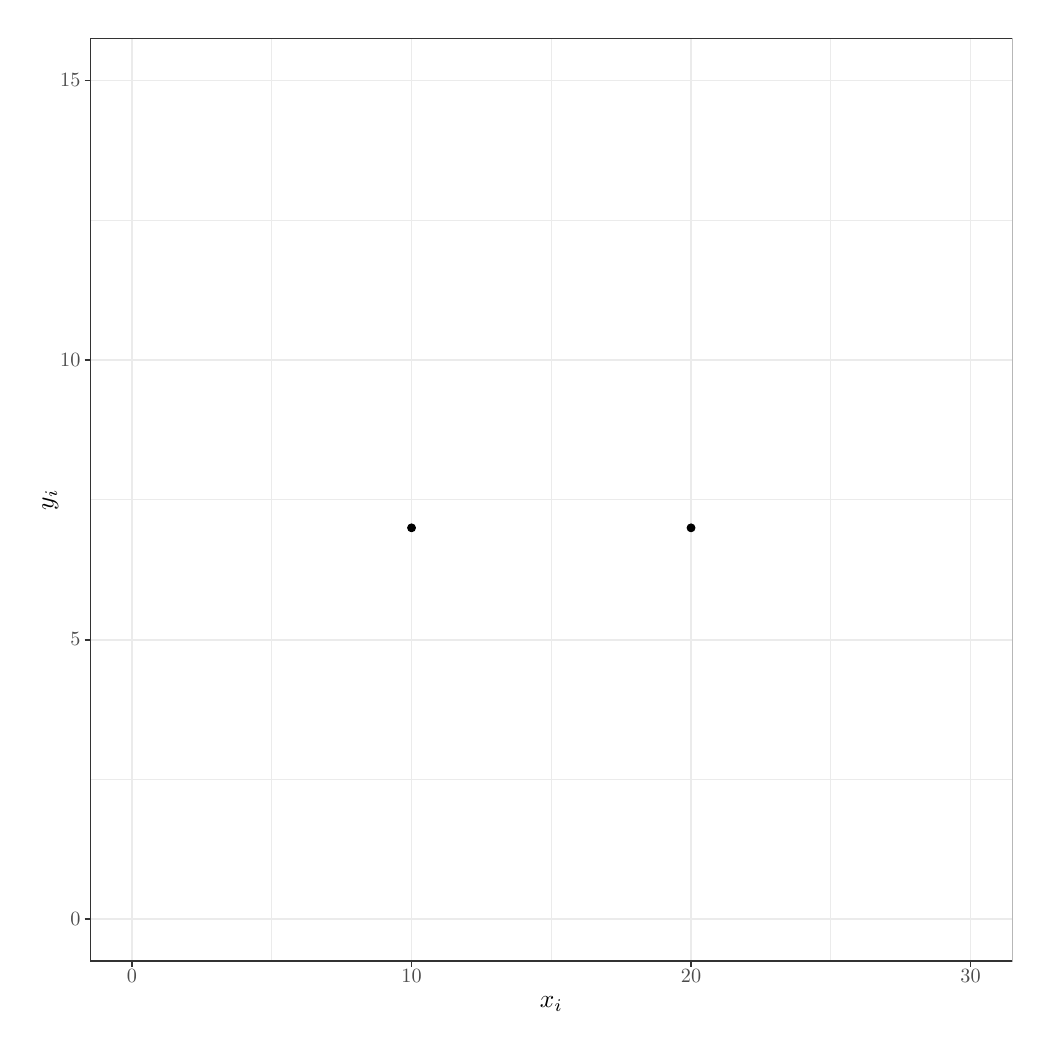
\begin{tikzpicture}[scale = 0.025]
% Created by tikzDevice version 0.12 on 2019-05-28 10:11:01
% !TEX encoding = UTF-8 Unicode
\definecolor{fillColor}{RGB}{255,255,255}
\path[use as bounding box,fill=fillColor,fill opacity=0.00] (0,0) rectangle (505.89,505.89);
\begin{scope}
\path[clip] (  0.00,  0.00) rectangle (505.89,505.89);
\definecolor{drawColor}{RGB}{255,255,255}
\definecolor{fillColor}{RGB}{255,255,255}

\path[draw=drawColor,line width= 0.6pt,line join=round,line cap=round,fill=fillColor] (  0.00,  0.00) rectangle (505.89,505.89);
\end{scope}
\begin{scope}
\path[clip] ( 31.73, 31.51) rectangle (500.39,500.39);
\definecolor{fillColor}{RGB}{255,255,255}

\path[fill=fillColor] ( 31.73, 31.51) rectangle (500.39,500.39);
\definecolor{drawColor}{gray}{0.92}

\path[draw=drawColor,line width= 0.3pt,line join=round] ( 31.73,123.86) --
	(500.39,123.86);

\path[draw=drawColor,line width= 0.3pt,line join=round] ( 31.73,265.95) --
	(500.39,265.95);

\path[draw=drawColor,line width= 0.3pt,line join=round] ( 31.73,408.03) --
	(500.39,408.03);

\path[draw=drawColor,line width= 0.3pt,line join=round] (124.04, 31.51) --
	(124.04,500.39);

\path[draw=drawColor,line width= 0.3pt,line join=round] (266.06, 31.51) --
	(266.06,500.39);

\path[draw=drawColor,line width= 0.3pt,line join=round] (408.08, 31.51) --
	(408.08,500.39);

\path[draw=drawColor,line width= 0.6pt,line join=round] ( 31.73, 52.82) --
	(500.39, 52.82);

\path[draw=drawColor,line width= 0.6pt,line join=round] ( 31.73,194.91) --
	(500.39,194.91);

\path[draw=drawColor,line width= 0.6pt,line join=round] ( 31.73,336.99) --
	(500.39,336.99);

\path[draw=drawColor,line width= 0.6pt,line join=round] ( 31.73,479.08) --
	(500.39,479.08);

\path[draw=drawColor,line width= 0.6pt,line join=round] ( 53.03, 31.51) --
	( 53.03,500.39);

\path[draw=drawColor,line width= 0.6pt,line join=round] (195.05, 31.51) --
	(195.05,500.39);

\path[draw=drawColor,line width= 0.6pt,line join=round] (337.07, 31.51) --
	(337.07,500.39);

\path[draw=drawColor,line width= 0.6pt,line join=round] (479.09, 31.51) --
	(479.09,500.39);
\definecolor{drawColor}{RGB}{0,0,0}
\definecolor{fillColor}{RGB}{0,0,0}

\path[draw=drawColor,line width= 0.4pt,line join=round,line cap=round,fill=fillColor] (195.05,251.74) circle (  1.96);

\path[draw=drawColor,line width= 0.4pt,line join=round,line cap=round,fill=fillColor] (337.07,251.74) circle (  1.96);
\definecolor{drawColor}{gray}{0.20}

\path[draw=drawColor,line width= 0.6pt,line join=round,line cap=round] ( 31.73, 31.51) rectangle (500.39,500.39);
\end{scope}
\begin{scope}
\path[clip] (  0.00,  0.00) rectangle (505.89,505.89);
\definecolor{drawColor}{gray}{0.30}

\node[text=drawColor,anchor=base east,inner sep=0pt, outer sep=0pt, scale=  0.73] at ( 26.78, 49.79) {0};

\node[text=drawColor,anchor=base east,inner sep=0pt, outer sep=0pt, scale=  0.73] at ( 26.78,191.87) {5};

\node[text=drawColor,anchor=base east,inner sep=0pt, outer sep=0pt, scale=  0.73] at ( 26.78,333.96) {10};

\node[text=drawColor,anchor=base east,inner sep=0pt, outer sep=0pt, scale=  0.73] at ( 26.78,476.05) {15};
\end{scope}
\begin{scope}
\path[clip] (  0.00,  0.00) rectangle (505.89,505.89);
\definecolor{drawColor}{gray}{0.20}

\path[draw=drawColor,line width= 0.6pt,line join=round] ( 28.98, 52.82) --
	( 31.73, 52.82);

\path[draw=drawColor,line width= 0.6pt,line join=round] ( 28.98,194.91) --
	( 31.73,194.91);

\path[draw=drawColor,line width= 0.6pt,line join=round] ( 28.98,336.99) --
	( 31.73,336.99);

\path[draw=drawColor,line width= 0.6pt,line join=round] ( 28.98,479.08) --
	( 31.73,479.08);
\end{scope}
\begin{scope}
\path[clip] (  0.00,  0.00) rectangle (505.89,505.89);
\definecolor{drawColor}{gray}{0.20}

\path[draw=drawColor,line width= 0.6pt,line join=round] ( 53.03, 28.76) --
	( 53.03, 31.51);

\path[draw=drawColor,line width= 0.6pt,line join=round] (195.05, 28.76) --
	(195.05, 31.51);

\path[draw=drawColor,line width= 0.6pt,line join=round] (337.07, 28.76) --
	(337.07, 31.51);

\path[draw=drawColor,line width= 0.6pt,line join=round] (479.09, 28.76) --
	(479.09, 31.51);
\end{scope}
\begin{scope}
\path[clip] (  0.00,  0.00) rectangle (505.89,505.89);
\definecolor{drawColor}{gray}{0.30}

\node[text=drawColor,anchor=base,inner sep=0pt, outer sep=0pt, scale=  0.73] at ( 53.03, 20.49) {0};

\node[text=drawColor,anchor=base,inner sep=0pt, outer sep=0pt, scale=  0.73] at (195.05, 20.49) {10};

\node[text=drawColor,anchor=base,inner sep=0pt, outer sep=0pt, scale=  0.73] at (337.07, 20.49) {20};

\node[text=drawColor,anchor=base,inner sep=0pt, outer sep=0pt, scale=  0.73] at (479.09, 20.49) {30};
\end{scope}
\begin{scope}
\path[clip] (  0.00,  0.00) rectangle (505.89,505.89);
\definecolor{drawColor}{RGB}{0,0,0}

\node[text=drawColor,anchor=base,inner sep=0pt, outer sep=0pt, scale=  0.92] at (266.06,  7.83) {$x_i$};
\end{scope}
\begin{scope}
\path[clip] (  0.00,  0.00) rectangle (505.89,505.89);
\definecolor{drawColor}{RGB}{0,0,0}

\node[text=drawColor,rotate= 90.00,anchor=base,inner sep=0pt, outer sep=0pt, scale=  0.92] at ( 13.08,265.95) {$y_i$};
\end{scope}

\end{tikzpicture}
\end{center}
\end{minipage}

\begin{enumerate}
\item Проведите линию регрессии.
\item Найдите все $\hy_i$, $RSS$, $R^2$.
\end{enumerate}

\begin{sol}
\end{sol}
\end{problem}

\begin{problem}
На плоскости изображены оба наблюдения:

\begin{minted}[mathescape,
               linenos,
               numbersep=5pt,
               frame=lines,
               framesep=2mm]{r}
data_2d <- tibble(
  x = c(10, 20),
  y = c(7, 12))

qplot(data = data_2d, x = x, y = y) + theme_bw() +
  xlab("$x_i$") + ylab("$y_i$") +
  scale_y_continuous(limits = c(0, 20)) +
  scale_x_continuous(limits = c(0, 30))
\end{minted}



\begin{minipage}{0.6\textwidth}
\begin{center}
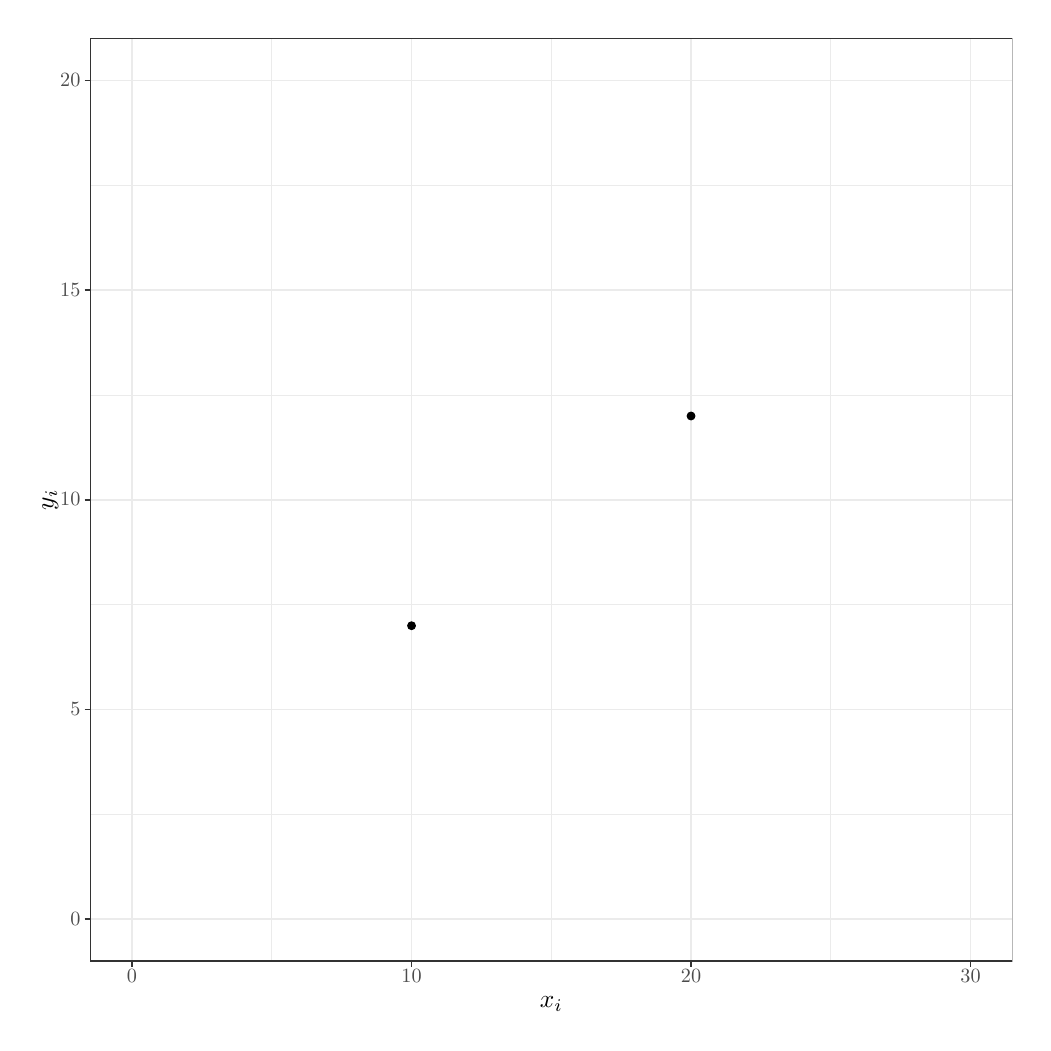
\begin{tikzpicture}[scale = 0.025]
% Created by tikzDevice version 0.12 on 2019-05-28 10:11:08
% !TEX encoding = UTF-8 Unicode
\definecolor{fillColor}{RGB}{255,255,255}
\path[use as bounding box,fill=fillColor,fill opacity=0.00] (0,0) rectangle (505.89,505.89);
\begin{scope}
\path[clip] (  0.00,  0.00) rectangle (505.89,505.89);
\definecolor{drawColor}{RGB}{255,255,255}
\definecolor{fillColor}{RGB}{255,255,255}

\path[draw=drawColor,line width= 0.6pt,line join=round,line cap=round,fill=fillColor] (  0.00,  0.00) rectangle (505.89,505.89);
\end{scope}
\begin{scope}
\path[clip] ( 31.73, 31.51) rectangle (500.39,500.39);
\definecolor{fillColor}{RGB}{255,255,255}

\path[fill=fillColor] ( 31.73, 31.51) rectangle (500.39,500.39);
\definecolor{drawColor}{gray}{0.92}

\path[draw=drawColor,line width= 0.3pt,line join=round] ( 31.73,106.10) --
	(500.39,106.10);

\path[draw=drawColor,line width= 0.3pt,line join=round] ( 31.73,212.67) --
	(500.39,212.67);

\path[draw=drawColor,line width= 0.3pt,line join=round] ( 31.73,319.23) --
	(500.39,319.23);

\path[draw=drawColor,line width= 0.3pt,line join=round] ( 31.73,425.79) --
	(500.39,425.79);

\path[draw=drawColor,line width= 0.3pt,line join=round] (124.04, 31.51) --
	(124.04,500.39);

\path[draw=drawColor,line width= 0.3pt,line join=round] (266.06, 31.51) --
	(266.06,500.39);

\path[draw=drawColor,line width= 0.3pt,line join=round] (408.08, 31.51) --
	(408.08,500.39);

\path[draw=drawColor,line width= 0.6pt,line join=round] ( 31.73, 52.82) --
	(500.39, 52.82);

\path[draw=drawColor,line width= 0.6pt,line join=round] ( 31.73,159.38) --
	(500.39,159.38);

\path[draw=drawColor,line width= 0.6pt,line join=round] ( 31.73,265.95) --
	(500.39,265.95);

\path[draw=drawColor,line width= 0.6pt,line join=round] ( 31.73,372.51) --
	(500.39,372.51);

\path[draw=drawColor,line width= 0.6pt,line join=round] ( 31.73,479.08) --
	(500.39,479.08);

\path[draw=drawColor,line width= 0.6pt,line join=round] ( 53.03, 31.51) --
	( 53.03,500.39);

\path[draw=drawColor,line width= 0.6pt,line join=round] (195.05, 31.51) --
	(195.05,500.39);

\path[draw=drawColor,line width= 0.6pt,line join=round] (337.07, 31.51) --
	(337.07,500.39);

\path[draw=drawColor,line width= 0.6pt,line join=round] (479.09, 31.51) --
	(479.09,500.39);
\definecolor{drawColor}{RGB}{0,0,0}
\definecolor{fillColor}{RGB}{0,0,0}

\path[draw=drawColor,line width= 0.4pt,line join=round,line cap=round,fill=fillColor] (195.05,202.01) circle (  1.96);

\path[draw=drawColor,line width= 0.4pt,line join=round,line cap=round,fill=fillColor] (337.07,308.57) circle (  1.96);
\definecolor{drawColor}{gray}{0.20}

\path[draw=drawColor,line width= 0.6pt,line join=round,line cap=round] ( 31.73, 31.51) rectangle (500.39,500.39);
\end{scope}
\begin{scope}
\path[clip] (  0.00,  0.00) rectangle (505.89,505.89);
\definecolor{drawColor}{gray}{0.30}

\node[text=drawColor,anchor=base east,inner sep=0pt, outer sep=0pt, scale=  0.73] at ( 26.78, 49.79) {0};

\node[text=drawColor,anchor=base east,inner sep=0pt, outer sep=0pt, scale=  0.73] at ( 26.78,156.35) {5};

\node[text=drawColor,anchor=base east,inner sep=0pt, outer sep=0pt, scale=  0.73] at ( 26.78,262.92) {10};

\node[text=drawColor,anchor=base east,inner sep=0pt, outer sep=0pt, scale=  0.73] at ( 26.78,369.48) {15};

\node[text=drawColor,anchor=base east,inner sep=0pt, outer sep=0pt, scale=  0.73] at ( 26.78,476.05) {20};
\end{scope}
\begin{scope}
\path[clip] (  0.00,  0.00) rectangle (505.89,505.89);
\definecolor{drawColor}{gray}{0.20}

\path[draw=drawColor,line width= 0.6pt,line join=round] ( 28.98, 52.82) --
	( 31.73, 52.82);

\path[draw=drawColor,line width= 0.6pt,line join=round] ( 28.98,159.38) --
	( 31.73,159.38);

\path[draw=drawColor,line width= 0.6pt,line join=round] ( 28.98,265.95) --
	( 31.73,265.95);

\path[draw=drawColor,line width= 0.6pt,line join=round] ( 28.98,372.51) --
	( 31.73,372.51);

\path[draw=drawColor,line width= 0.6pt,line join=round] ( 28.98,479.08) --
	( 31.73,479.08);
\end{scope}
\begin{scope}
\path[clip] (  0.00,  0.00) rectangle (505.89,505.89);
\definecolor{drawColor}{gray}{0.20}

\path[draw=drawColor,line width= 0.6pt,line join=round] ( 53.03, 28.76) --
	( 53.03, 31.51);

\path[draw=drawColor,line width= 0.6pt,line join=round] (195.05, 28.76) --
	(195.05, 31.51);

\path[draw=drawColor,line width= 0.6pt,line join=round] (337.07, 28.76) --
	(337.07, 31.51);

\path[draw=drawColor,line width= 0.6pt,line join=round] (479.09, 28.76) --
	(479.09, 31.51);
\end{scope}
\begin{scope}
\path[clip] (  0.00,  0.00) rectangle (505.89,505.89);
\definecolor{drawColor}{gray}{0.30}

\node[text=drawColor,anchor=base,inner sep=0pt, outer sep=0pt, scale=  0.73] at ( 53.03, 20.49) {0};

\node[text=drawColor,anchor=base,inner sep=0pt, outer sep=0pt, scale=  0.73] at (195.05, 20.49) {10};

\node[text=drawColor,anchor=base,inner sep=0pt, outer sep=0pt, scale=  0.73] at (337.07, 20.49) {20};

\node[text=drawColor,anchor=base,inner sep=0pt, outer sep=0pt, scale=  0.73] at (479.09, 20.49) {30};
\end{scope}
\begin{scope}
\path[clip] (  0.00,  0.00) rectangle (505.89,505.89);
\definecolor{drawColor}{RGB}{0,0,0}

\node[text=drawColor,anchor=base,inner sep=0pt, outer sep=0pt, scale=  0.92] at (266.06,  7.83) {$x_i$};
\end{scope}
\begin{scope}
\path[clip] (  0.00,  0.00) rectangle (505.89,505.89);
\definecolor{drawColor}{RGB}{0,0,0}

\node[text=drawColor,rotate= 90.00,anchor=base,inner sep=0pt, outer sep=0pt, scale=  0.92] at ( 13.08,265.95) {$y_i$};
\end{scope}

\end{tikzpicture}
\end{center}
\end{minipage}

\begin{enumerate}
\item Проведите линию регрессии.
\item Найдите $RSS$, $R^2$.
\end{enumerate}

\begin{sol}
\end{sol}
\end{problem}


\begin{problem}
Три точки, прямая $\hy_i = \hb_1 + \hb_2 x_i$. Даны два расстояния от точек до прямой по вертикали, надо найти третье.
\todo[inline]{вставить график}
\begin{sol}
Вспомним, что сумма остатков регрессии равна нулю.
\end{sol}
\end{problem}

\begin{problem}
На работе Эконометресса Эвридика построила парную регрессию по трём наблюдениям. На листочек она переписала фактические значения $y_i$ и прогнозные $\hy_i$. К сожалению, когда Эвридика пришла домой, она обнаружила, что слишком неразборчиво записала два значения $\hy_i$:

\begin{tabular}{rr}
\toprule
$y_i$ & $\hy_i$ \\
\midrule
$0$ & $5$ \\
$10$ & ? \\
$20$ & ? \\
\bottomrule
\end{tabular}

\begin{enumerate}
\item Восстановите пропущенные значения.
\item Найдите $RSS$, $ESS$, $TSS$, $R^2$.
\end{enumerate}


\begin{sol}
Остатки $\hat u_i = y_i - \hy_i$ должны быть ортогональны вектору из единичек и вектору $\hy$. То есть получаем систему уравнений
\[
\begin{cases}
\sum_i (y_i - \hy_i) = 0 \\
\sum_i (y_i - \hy_i) \hy_i = 0 \\
\end{cases}
\]

\end{sol}
\end{problem}

\begin{problem}
На плоскости изображены наблюдения и линия регрессии:



\begin{minted}[mathescape,
               linenos,
               numbersep=5pt,
               frame=lines,
               framesep=2mm]{r}
set.seed(94)
n_obs <- 20
data_2d <- tibble(
  x = -20 + rbinom(n_obs, size = 50, prob = 0.5),
  y = 5 + 3 * x + rbinom(n_obs, size = 160, prob = 0.5))

x_bar <- mean(data_2d$x)

qplot(data = data_2d, x = x, y = y) + theme_bw() +
  scale_x_continuous(breaks = c(0, data_2d$x[20], x_bar),
                     labels = c("$0$", "$x_{20}$", "$\\bar x$")) +
  stat_smooth(method = "lm", se = FALSE, col = I("gray")) +
  xlab("") + ylab("$y_i$")
\end{minted}




\begin{minipage}{\textwidth}
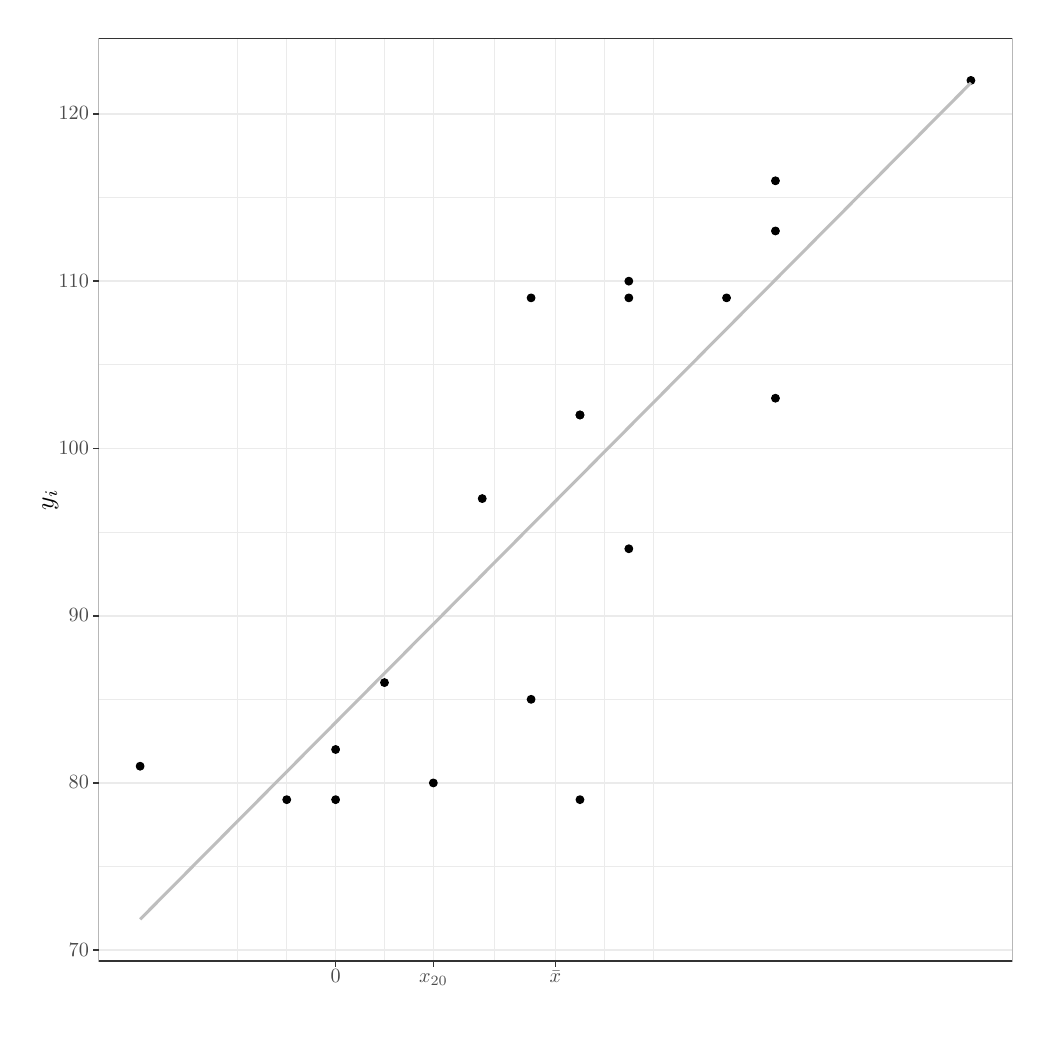
\begin{tikzpicture}[scale = 0.025]
% Created by tikzDevice version 0.12 on 2019-05-28 10:11:09
% !TEX encoding = UTF-8 Unicode
\definecolor{fillColor}{RGB}{255,255,255}
\path[use as bounding box,fill=fillColor,fill opacity=0.00] (0,0) rectangle (505.89,505.89);
\begin{scope}
\path[clip] (  0.00,  0.00) rectangle (505.89,505.89);
\definecolor{drawColor}{RGB}{255,255,255}
\definecolor{fillColor}{RGB}{255,255,255}

\path[draw=drawColor,line width= 0.6pt,line join=round,line cap=round,fill=fillColor] (  0.00,  0.00) rectangle (505.89,505.89);
\end{scope}
\begin{scope}
\path[clip] ( 36.04, 31.51) rectangle (500.39,500.39);
\definecolor{fillColor}{RGB}{255,255,255}

\path[fill=fillColor] ( 36.04, 31.51) rectangle (500.39,500.39);
\definecolor{drawColor}{gray}{0.92}

\path[draw=drawColor,line width= 0.3pt,line join=round] ( 36.04, 79.62) --
	(500.39, 79.62);

\path[draw=drawColor,line width= 0.3pt,line join=round] ( 36.04,164.61) --
	(500.39,164.61);

\path[draw=drawColor,line width= 0.3pt,line join=round] ( 36.04,249.60) --
	(500.39,249.60);

\path[draw=drawColor,line width= 0.3pt,line join=round] ( 36.04,334.59) --
	(500.39,334.59);

\path[draw=drawColor,line width= 0.3pt,line join=round] ( 36.04,419.58) --
	(500.39,419.58);

\path[draw=drawColor,line width= 0.3pt,line join=round] (106.81, 31.51) --
	(106.81,500.39);

\path[draw=drawColor,line width= 0.3pt,line join=round] (131.64, 31.51) --
	(131.64,500.39);

\path[draw=drawColor,line width= 0.3pt,line join=round] (181.30, 31.51) --
	(181.30,500.39);

\path[draw=drawColor,line width= 0.3pt,line join=round] (237.17, 31.51) --
	(237.17,500.39);

\path[draw=drawColor,line width= 0.3pt,line join=round] (293.04, 31.51) --
	(293.04,500.39);

\path[draw=drawColor,line width= 0.3pt,line join=round] (317.88, 31.51) --
	(317.88,500.39);

\path[draw=drawColor,line width= 0.6pt,line join=round] ( 36.04, 37.13) --
	(500.39, 37.13);

\path[draw=drawColor,line width= 0.6pt,line join=round] ( 36.04,122.12) --
	(500.39,122.12);

\path[draw=drawColor,line width= 0.6pt,line join=round] ( 36.04,207.11) --
	(500.39,207.11);

\path[draw=drawColor,line width= 0.6pt,line join=round] ( 36.04,292.10) --
	(500.39,292.10);

\path[draw=drawColor,line width= 0.6pt,line join=round] ( 36.04,377.09) --
	(500.39,377.09);

\path[draw=drawColor,line width= 0.6pt,line join=round] ( 36.04,462.08) --
	(500.39,462.08);

\path[draw=drawColor,line width= 0.6pt,line join=round] (156.47, 31.51) --
	(156.47,500.39);

\path[draw=drawColor,line width= 0.6pt,line join=round] (206.13, 31.51) --
	(206.13,500.39);

\path[draw=drawColor,line width= 0.6pt,line join=round] (268.21, 31.51) --
	(268.21,500.39);
\definecolor{drawColor}{RGB}{0,0,0}
\definecolor{fillColor}{RGB}{0,0,0}

\path[draw=drawColor,line width= 0.4pt,line join=round,line cap=round,fill=fillColor] (379.96,428.08) circle (  1.96);

\path[draw=drawColor,line width= 0.4pt,line join=round,line cap=round,fill=fillColor] (280.63,113.62) circle (  1.96);

\path[draw=drawColor,line width= 0.4pt,line join=round,line cap=round,fill=fillColor] (305.46,241.11) circle (  1.96);

\path[draw=drawColor,line width= 0.4pt,line join=round,line cap=round,fill=fillColor] (305.46,368.59) circle (  1.96);

\path[draw=drawColor,line width= 0.4pt,line join=round,line cap=round,fill=fillColor] (156.47,139.12) circle (  1.96);

\path[draw=drawColor,line width= 0.4pt,line join=round,line cap=round,fill=fillColor] (280.63,309.10) circle (  1.96);

\path[draw=drawColor,line width= 0.4pt,line join=round,line cap=round,fill=fillColor] (379.96,317.60) circle (  1.96);

\path[draw=drawColor,line width= 0.4pt,line join=round,line cap=round,fill=fillColor] (479.28,479.08) circle (  1.96);

\path[draw=drawColor,line width= 0.4pt,line join=round,line cap=round,fill=fillColor] (181.30,173.11) circle (  1.96);

\path[draw=drawColor,line width= 0.4pt,line join=round,line cap=round,fill=fillColor] (305.46,377.09) circle (  1.96);

\path[draw=drawColor,line width= 0.4pt,line join=round,line cap=round,fill=fillColor] (280.63,309.10) circle (  1.96);

\path[draw=drawColor,line width= 0.4pt,line join=round,line cap=round,fill=fillColor] (230.97,266.60) circle (  1.96);

\path[draw=drawColor,line width= 0.4pt,line join=round,line cap=round,fill=fillColor] (255.80,368.59) circle (  1.96);

\path[draw=drawColor,line width= 0.4pt,line join=round,line cap=round,fill=fillColor] (131.64,113.62) circle (  1.96);

\path[draw=drawColor,line width= 0.4pt,line join=round,line cap=round,fill=fillColor] (355.12,368.59) circle (  1.96);

\path[draw=drawColor,line width= 0.4pt,line join=round,line cap=round,fill=fillColor] (156.47,113.62) circle (  1.96);

\path[draw=drawColor,line width= 0.4pt,line join=round,line cap=round,fill=fillColor] (379.96,402.59) circle (  1.96);

\path[draw=drawColor,line width= 0.4pt,line join=round,line cap=round,fill=fillColor] (255.80,164.61) circle (  1.96);

\path[draw=drawColor,line width= 0.4pt,line join=round,line cap=round,fill=fillColor] ( 57.14,130.62) circle (  1.96);

\path[draw=drawColor,line width= 0.4pt,line join=round,line cap=round,fill=fillColor] (206.13,122.12) circle (  1.96);
\definecolor{drawColor}{RGB}{190,190,190}

\path[draw=drawColor,line width= 1.1pt,line join=round] ( 57.14, 52.82) --
	( 62.49, 58.20) --
	( 67.83, 63.58) --
	( 73.17, 68.96) --
	( 78.52, 74.34) --
	( 83.86, 79.72) --
	( 89.20, 85.10) --
	( 94.55, 90.48) --
	( 99.89, 95.86) --
	(105.23,101.24) --
	(110.58,106.62) --
	(115.92,112.00) --
	(121.27,117.38) --
	(126.61,122.76) --
	(131.95,128.14) --
	(137.30,133.52) --
	(142.64,138.90) --
	(147.98,144.28) --
	(153.33,149.66) --
	(158.67,155.04) --
	(164.01,160.42) --
	(169.36,165.80) --
	(174.70,171.18) --
	(180.04,176.56) --
	(185.39,181.94) --
	(190.73,187.32) --
	(196.07,192.70) --
	(201.42,198.08) --
	(206.76,203.46) --
	(212.11,208.84) --
	(217.45,214.22) --
	(222.79,219.60) --
	(228.14,224.98) --
	(233.48,230.36) --
	(238.82,235.74) --
	(244.17,241.12) --
	(249.51,246.50) --
	(254.85,251.88) --
	(260.20,257.26) --
	(265.54,262.64) --
	(270.88,268.02) --
	(276.23,273.40) --
	(281.57,278.78) --
	(286.92,284.16) --
	(292.26,289.54) --
	(297.60,294.92) --
	(302.95,300.30) --
	(308.29,305.68) --
	(313.63,311.06) --
	(318.98,316.44) --
	(324.32,321.82) --
	(329.66,327.20) --
	(335.01,332.58) --
	(340.35,337.96) --
	(345.69,343.34) --
	(351.04,348.72) --
	(356.38,354.10) --
	(361.72,359.48) --
	(367.07,364.86) --
	(372.41,370.24) --
	(377.76,375.62) --
	(383.10,381.00) --
	(388.44,386.38) --
	(393.79,391.76) --
	(399.13,397.14) --
	(404.47,402.52) --
	(409.82,407.90) --
	(415.16,413.28) --
	(420.50,418.66) --
	(425.85,424.04) --
	(431.19,429.42) --
	(436.53,434.80) --
	(441.88,440.18) --
	(447.22,445.56) --
	(452.57,450.94) --
	(457.91,456.32) --
	(463.25,461.70) --
	(468.60,467.08) --
	(473.94,472.46) --
	(479.28,477.84);
\definecolor{drawColor}{gray}{0.20}

\path[draw=drawColor,line width= 0.6pt,line join=round,line cap=round] ( 36.04, 31.51) rectangle (500.39,500.39);
\end{scope}
\begin{scope}
\path[clip] (  0.00,  0.00) rectangle (505.89,505.89);
\definecolor{drawColor}{gray}{0.30}

\node[text=drawColor,anchor=base east,inner sep=0pt, outer sep=0pt, scale=  0.73] at ( 31.09, 34.10) {70};

\node[text=drawColor,anchor=base east,inner sep=0pt, outer sep=0pt, scale=  0.73] at ( 31.09,119.09) {80};

\node[text=drawColor,anchor=base east,inner sep=0pt, outer sep=0pt, scale=  0.73] at ( 31.09,204.08) {90};

\node[text=drawColor,anchor=base east,inner sep=0pt, outer sep=0pt, scale=  0.73] at ( 31.09,289.07) {100};

\node[text=drawColor,anchor=base east,inner sep=0pt, outer sep=0pt, scale=  0.73] at ( 31.09,374.06) {110};

\node[text=drawColor,anchor=base east,inner sep=0pt, outer sep=0pt, scale=  0.73] at ( 31.09,459.05) {120};
\end{scope}
\begin{scope}
\path[clip] (  0.00,  0.00) rectangle (505.89,505.89);
\definecolor{drawColor}{gray}{0.20}

\path[draw=drawColor,line width= 0.6pt,line join=round] ( 33.29, 37.13) --
	( 36.04, 37.13);

\path[draw=drawColor,line width= 0.6pt,line join=round] ( 33.29,122.12) --
	( 36.04,122.12);

\path[draw=drawColor,line width= 0.6pt,line join=round] ( 33.29,207.11) --
	( 36.04,207.11);

\path[draw=drawColor,line width= 0.6pt,line join=round] ( 33.29,292.10) --
	( 36.04,292.10);

\path[draw=drawColor,line width= 0.6pt,line join=round] ( 33.29,377.09) --
	( 36.04,377.09);

\path[draw=drawColor,line width= 0.6pt,line join=round] ( 33.29,462.08) --
	( 36.04,462.08);
\end{scope}
\begin{scope}
\path[clip] (  0.00,  0.00) rectangle (505.89,505.89);
\definecolor{drawColor}{gray}{0.20}

\path[draw=drawColor,line width= 0.6pt,line join=round] (156.47, 28.76) --
	(156.47, 31.51);

\path[draw=drawColor,line width= 0.6pt,line join=round] (206.13, 28.76) --
	(206.13, 31.51);

\path[draw=drawColor,line width= 0.6pt,line join=round] (268.21, 28.76) --
	(268.21, 31.51);
\end{scope}
\begin{scope}
\path[clip] (  0.00,  0.00) rectangle (505.89,505.89);
\definecolor{drawColor}{gray}{0.30}

\node[text=drawColor,anchor=base,inner sep=0pt, outer sep=0pt, scale=  0.73] at (156.47, 20.49) {$0$};

\node[text=drawColor,anchor=base,inner sep=0pt, outer sep=0pt, scale=  0.73] at (206.13, 20.49) {$x_{20}$};

\node[text=drawColor,anchor=base,inner sep=0pt, outer sep=0pt, scale=  0.73] at (268.21, 20.49) {$\bar x$};
\end{scope}
\begin{scope}
\path[clip] (  0.00,  0.00) rectangle (505.89,505.89);
\definecolor{drawColor}{RGB}{0,0,0}

\node[text=drawColor,rotate= 90.00,anchor=base,inner sep=0pt, outer sep=0pt, scale=  0.92] at ( 13.08,265.95) {$y_i$};
\end{scope}

\end{tikzpicture}
\end{minipage}


\begin{enumerate}
\item Изобразите на плоскости $\hy_{20}$, $y_{20}$, $\bar y$, $\hat u_{20}$, $\hb_1$.
\item Что произойдёт с каждой из указанных величин при добавлении нового наблюдения равного $(\bar x + 1, \bar y + \hb_2)$?
\end{enumerate}
\begin{sol}
Добавляемое наблюдение лежит на линии регрессии, поэтому ничего не изменится.
\end{sol}
\end{problem}


\begin{problem}
  Имеется всего два наблюдения, $y_1 = 1$, $y_2 = -3$. С помощью критериев $AIC$ и $BIC$ сравните две модели. Модель А: $y_i \sim \cN(0; 1)$ и независимы, модель Б: $y_i \sim \cN(\mu; 1)$ и независимы.
\begin{sol}
  $RSS_A = 1^2 + (-3)^2 = 10$, $RSS_B= 2^2 + 2^2 = 8$. $k_A = 0$, $k_B=1$.
\end{sol}
\end{problem}


\begin{problem}
Постройте парную регрессию по четырём наблюдениям:

\begin{minted}[mathescape,
               linenos,
               numbersep=5pt,
               frame=lines,
               framesep=2mm]{r}
data_2d <- tibble(
  x = c(1, 2, 2, 2),
  y = c(3, 1, 2, 3))

qplot(data = data_2d, x = x, y = y) + theme_bw() +
  scale_x_continuous(breaks = c(0, 1, 2),
  labels = c("$0$", "$1$", "$2$")) +
  xlab("$x_i$") + ylab("$y_i$")
\end{minted}


\begin{minipage}{\textwidth}
\begin{tikzpicture}[scale = 0.025]
% Created by tikzDevice version 0.12 on 2019-05-28 10:11:22
% !TEX encoding = UTF-8 Unicode
\definecolor{fillColor}{RGB}{255,255,255}
\path[use as bounding box,fill=fillColor,fill opacity=0.00] (0,0) rectangle (505.89,505.89);
\begin{scope}
\path[clip] (  0.00,  0.00) rectangle (505.89,505.89);
\definecolor{drawColor}{RGB}{255,255,255}
\definecolor{fillColor}{RGB}{255,255,255}

\path[draw=drawColor,line width= 0.6pt,line join=round,line cap=round,fill=fillColor] (  0.00,  0.00) rectangle (505.89,505.89);
\end{scope}
\begin{scope}
\path[clip] ( 34.12, 31.51) rectangle (500.39,500.39);
\definecolor{fillColor}{RGB}{255,255,255}

\path[fill=fillColor] ( 34.12, 31.51) rectangle (500.39,500.39);
\definecolor{drawColor}{gray}{0.92}

\path[draw=drawColor,line width= 0.3pt,line join=round] ( 34.12,106.10) --
	(500.39,106.10);

\path[draw=drawColor,line width= 0.3pt,line join=round] ( 34.12,212.67) --
	(500.39,212.67);

\path[draw=drawColor,line width= 0.3pt,line join=round] ( 34.12,319.23) --
	(500.39,319.23);

\path[draw=drawColor,line width= 0.3pt,line join=round] ( 34.12,425.79) --
	(500.39,425.79);

\path[draw=drawColor,line width= 0.3pt,line join=round] (267.26, 31.51) --
	(267.26,500.39);

\path[draw=drawColor,line width= 0.6pt,line join=round] ( 34.12, 52.82) --
	(500.39, 52.82);

\path[draw=drawColor,line width= 0.6pt,line join=round] ( 34.12,159.38) --
	(500.39,159.38);

\path[draw=drawColor,line width= 0.6pt,line join=round] ( 34.12,265.95) --
	(500.39,265.95);

\path[draw=drawColor,line width= 0.6pt,line join=round] ( 34.12,372.51) --
	(500.39,372.51);

\path[draw=drawColor,line width= 0.6pt,line join=round] ( 34.12,479.08) --
	(500.39,479.08);

\path[draw=drawColor,line width= 0.6pt,line join=round] ( 55.32, 31.51) --
	( 55.32,500.39);

\path[draw=drawColor,line width= 0.6pt,line join=round] (479.20, 31.51) --
	(479.20,500.39);
\definecolor{drawColor}{RGB}{0,0,0}
\definecolor{fillColor}{RGB}{0,0,0}

\path[draw=drawColor,line width= 0.4pt,line join=round,line cap=round,fill=fillColor] ( 55.32,479.08) circle (  1.96);

\path[draw=drawColor,line width= 0.4pt,line join=round,line cap=round,fill=fillColor] (479.20, 52.82) circle (  1.96);

\path[draw=drawColor,line width= 0.4pt,line join=round,line cap=round,fill=fillColor] (479.20,265.95) circle (  1.96);

\path[draw=drawColor,line width= 0.4pt,line join=round,line cap=round,fill=fillColor] (479.20,479.08) circle (  1.96);
\definecolor{drawColor}{gray}{0.20}

\path[draw=drawColor,line width= 0.6pt,line join=round,line cap=round] ( 34.12, 31.51) rectangle (500.39,500.39);
\end{scope}
\begin{scope}
\path[clip] (  0.00,  0.00) rectangle (505.89,505.89);
\definecolor{drawColor}{gray}{0.30}

\node[text=drawColor,anchor=base east,inner sep=0pt, outer sep=0pt, scale=  0.73] at ( 29.17, 49.79) {1.0};

\node[text=drawColor,anchor=base east,inner sep=0pt, outer sep=0pt, scale=  0.73] at ( 29.17,156.35) {1.5};

\node[text=drawColor,anchor=base east,inner sep=0pt, outer sep=0pt, scale=  0.73] at ( 29.17,262.92) {2.0};

\node[text=drawColor,anchor=base east,inner sep=0pt, outer sep=0pt, scale=  0.73] at ( 29.17,369.48) {2.5};

\node[text=drawColor,anchor=base east,inner sep=0pt, outer sep=0pt, scale=  0.73] at ( 29.17,476.05) {3.0};
\end{scope}
\begin{scope}
\path[clip] (  0.00,  0.00) rectangle (505.89,505.89);
\definecolor{drawColor}{gray}{0.20}

\path[draw=drawColor,line width= 0.6pt,line join=round] ( 31.37, 52.82) --
	( 34.12, 52.82);

\path[draw=drawColor,line width= 0.6pt,line join=round] ( 31.37,159.38) --
	( 34.12,159.38);

\path[draw=drawColor,line width= 0.6pt,line join=round] ( 31.37,265.95) --
	( 34.12,265.95);

\path[draw=drawColor,line width= 0.6pt,line join=round] ( 31.37,372.51) --
	( 34.12,372.51);

\path[draw=drawColor,line width= 0.6pt,line join=round] ( 31.37,479.08) --
	( 34.12,479.08);
\end{scope}
\begin{scope}
\path[clip] (  0.00,  0.00) rectangle (505.89,505.89);
\definecolor{drawColor}{gray}{0.20}

\path[draw=drawColor,line width= 0.6pt,line join=round] ( 55.32, 28.76) --
	( 55.32, 31.51);

\path[draw=drawColor,line width= 0.6pt,line join=round] (479.20, 28.76) --
	(479.20, 31.51);
\end{scope}
\begin{scope}
\path[clip] (  0.00,  0.00) rectangle (505.89,505.89);
\definecolor{drawColor}{gray}{0.30}

\node[text=drawColor,anchor=base,inner sep=0pt, outer sep=0pt, scale=  0.73] at ( 55.32, 20.49) {$1$};

\node[text=drawColor,anchor=base,inner sep=0pt, outer sep=0pt, scale=  0.73] at (479.20, 20.49) {$2$};
\end{scope}
\begin{scope}
\path[clip] (  0.00,  0.00) rectangle (505.89,505.89);
\definecolor{drawColor}{RGB}{0,0,0}

\node[text=drawColor,anchor=base,inner sep=0pt, outer sep=0pt, scale=  0.92] at (267.26,  7.83) {$x_i$};
\end{scope}
\begin{scope}
\path[clip] (  0.00,  0.00) rectangle (505.89,505.89);
\definecolor{drawColor}{RGB}{0,0,0}

\node[text=drawColor,rotate= 90.00,anchor=base,inner sep=0pt, outer sep=0pt, scale=  0.92] at ( 13.08,265.95) {$y_i$};
\end{scope}

\end{tikzpicture}
\end{minipage}


\begin{sol}
$\hy_i = 4 - x_i$
\end{sol}
\end{problem}


\begin{problem}
Исследователь Василий повторяет четыре раза оригинальный случайный эксперимент.
Эксперимент состоит в подбрасывании 10 стандартных игральных кубиков.
Количество выпавших единиц в $i$-м эксперименте — случайная величина $x_i$,
количество выпавших двоек — $z_i$,
суммарное количество четвёрок, пятёрок и шестёрок — $y_i$.


Василий аккуратно собрал фактические данные:

\begin{tabular}{ccc}
\toprule
$x_i$ & $y_i$ & $z_i$ \\
\midrule
2 & 6 & 1 \\
1 & 7 & 0 \\
1 & 4 & 3 \\
2 & 5 & 2 \\
\bottomrule
\end{tabular}


\begin{enumerate}
\item Найдите теоретическое математическое ожидание $\E(x_i)$ и выборочное среднее $\bar x$.
\item Найдите теоретическую дисперсию $\Var(x_i)$ и выборочную дисперсию $\sVar(x)$.
\item Найдите теоретическую ковариацию $\Cov(x_i, y_i)$ и выборочную ковариацию $\sCov(x, y)$.
\item Найдите теоретическую корреляцию $\Corr(x_i, y_i)$ и выборочную корреляцию $\sCorr(x, y)$.
\item Найдите истинные коэффициенты $\beta_1$ и $\beta_2$ в модели $y_i = \beta_1 + \beta_2 x_i + u_i$ и оценки коэффициентов $\hb_1$ и $\hb_2$.
\item Найдите истинные коэффициенты $\gamma_1$ и $\gamma_2$ в модели $x_i = \gamma_1 + \gamma_2 y_i + u_i$ и оценки коэффициентов $\hat\gamma_1$ и $\hat\gamma_2$.
\item Как связаны между собой $\Corr(x_i, y_i)$, $\beta_2$ и $\gamma_2$?
\item Как связаны между собой $\sCorr(x, y)$, $\hb_2$ и $\hat\gamma_2$?
\item Найдите истинные коэффициенты $\alpha_1$, $\alpha_2$ и $\alpha_3$ в модели $y_i = \alpha_1 + \alpha_2 x_i + \alpha_3 z_i +  u_i$ и оценки коэффициентов $\hat\alpha_1$, $\hat\alpha_2$ и $\hat\alpha_3$.
\item Найдите истинные коэффициенты $\delta_1$, $\delta_2$ и $\delta_3$ в модели $x_i = \delta_1 + \delta_2 y_i + \delta_3 z_i +  u_i$ и оценки коэффициентов $\hat\delta_1$, $\hat\delta_2$ и $\hat\delta_3$.
\item Найдите теоретическую частную корреляцию $\pCorr(x_i, y_i; z_i)$ и выборочную частную корреляцию $\spCorr(x, y; z)$.
\item Почему для истинных характеристик мы пишем $x_i$, с индексом, а для выборочных — $x$,
без индекса?
\end{enumerate}

\begin{sol}
$\E(x_i)=10/6$, $\Var(x_i)=50/6$.
\end{sol}
\end{problem}

\begin{problem}
Машенька построила парную регрессию по 11 наблюдениям с $R^2=0.95$. Чтобы напакостить Машеньке, Вовочка переставил в случайном порядке значения зависимой переменной и предложил Машеньке заново оценить модель.

Какой ожидаемый $R^2$ получит Машенька?
\begin{sol}
Без ограничения общности центрируем исходные переменные. 
Значения регрессора обозначим $x_i$, исходную зависимую переменную $\tilde{y}_i$, а переставленную в случайном порядке $y_i$. 
По условию $\sum y_i^2 = \sum \tilde{y}_i^2$.

Фиксируем исходные переменные и находим:
\[
\E(R^2 | \tilde{y}) = \E\left( \frac{(\sum x_i y_i )^2}{\sum x_i^2 \sum y_i^2}  \right) = 
\frac{\Var(\sum x_i y_i | \tilde{y})}{\sum x_i^2 \sum y_i^2}
\]

Для начала найдём дисперсию отдельного игрека:
\[
\Var(y_i | \tilde{y}) = \frac{\sum \tilde{y}_i^2}{n} = \frac{\sum y_i^2}{n}
\]

А теперь из $\Cov(y_1, \sum y_i | \tilde{y}) =0$ найдём и дисперсию нужной суммы:
\[
\Var(\sum x_i y_i | \tilde{y}) = 
\Var(y_i | \tilde{y}) \left(  \sum x_i^2 - \sum_{i\neq j} x_i x_j \frac{1}{n-1}  \right) = 
\Var(y_i | \tilde{y}) \frac{n}{n-1} \sum x_i^2 = \frac{\sum x_i^2 \sum y_i^2 }{n-1}
\]

Заканчиваем подсчёт,
\[
\E(R^2 | \tilde{y}) = \frac{1}{n-1}
\]

Следовательно, и $\E(R^2) = \frac{1}{n-1} = 0.1$.
\end{sol}
\end{problem}

\begin{problem}
	Винни-Пух оценивает регрессию $\hy_t = \hb y_{t-1}$ с помощью метода наименьших квадратов.
	Найдите $\plim \hb$, если
\begin{enumerate}
	\item $y_t$ независимы и одинаково распределены $\cN(0; 1)$;
	\item $y_t$ независимы и одинаково распределены $\cN(1; 1)$;
	\item $y_t$ независимы и одинаково распределены $\cN(t; 1)$;
	\item $y_t$ независимы и одинаково распределены $\cN(1; t)$;
	\item $y_t$ независимы и одинаково распределены $\cN(t; t)$;
	\item $y_t = t$;
	\item $y_1 = 1$, а начиная с $t=2$ все $y_t=0$;
	\item $y_1 = 0$, а начиная с $t=2$ все $y_t=1$;
	\item $y_t = 1/t$;
	\item $y_t = t^2$;
	\item $y_t= 2^t$;
	\item $y_t = w_1 + w_2 + w_3 + \cdot + w_t$, где $w_t$ независимы и одинаково распределены;
	\item $y_t$ — это числа Фибоначчи;
\end{enumerate}

\begin{sol}
\end{sol}
\end{problem}

\begin{problem}
Илон Маск оценил модель парной регрессии $y_i = \b_1 + \b_2 x_i + u_i$.
Часть данных и прогнозов окалазась потеряна. 

\begin{tabular}{ccc}
  \toprule
  $x_i$ & $y_i$ & $\hy_i$ \\
  \midrule
  $a$ & 6 & 1 \\
  1 & 7 & 0 \\
  1 & 4 & 3 \\
  2 & 5 & $b$ \\
  \bottomrule
\end{tabular}
  
Помогите бравому Илону Маску восстановить пропуски, найдите $a$ и $b$. 
\begin{sol}
Решаем систему двух уравнений:
\[
\begin{cases}
  \langle x, y - \hy \rangle = 0, \\
  \langle \ones, y - \hy \rangle = 0 
\end{cases}
\]

Из $\langle \ones, y - \hy \rangle = 0$ следует, что $b=18$. 
Затем из $\langle x, y - \hy \rangle = 0$ следует, что $a=18/5$.
\end{sol}
\end{problem}





\Closesolutionfile{solution_file}
